\documentclass[a4paper]{article}
\usepackage[hmargin=1in, vmargin=1in]{geometry}
\usepackage{makeidx}
\usepackage{fancyhdr}
\pagestyle{fancy}
\usepackage[pdftex]{graphicx}
\usepackage{amsmath}
\usepackage{amssymb}
\usepackage{listings}
\usepackage{natbib}
%\usepackage{etex}
%\usepackage{m-pictex}
\makeindex

\begin{document}
\begin{center}

%
% - prelim (math defs)
%	- space
%	- basis
%	- normalisation
%		- norm to measuret
%
%	- cosine/sine (orthogonal complement property of the unit circles right angled triangles)
%	- 
%	- 
%
% - construction of a coordinate system 2x3 and mxn following
% - matrix (operator, TD, RT), functions (derivative, integral), functionals (y_n functionals)
%
% - corollaries:
% - n axes of m-dim in spherical coordinates with one r and m-1 angles are complementary by construction
% - embedding m-dim in m-dim
% - mapping n-dim onto m-dim
% - mapping n-dim onto 2-D (gen. for sphere, gen for any)
% - coordinate functionals
% - non-orthogonal basis


\title{m by n matrices. Coordinate functionals. Non-orthogonal map bases. }\\
\author{Edward Gerhold}

m by n matrices. Coordinate functionals. Non-orthogonal map bases. 

Formerly entitled  "Three dimensional coordinates into two dimensional coordinates transformation".

"m by n matrices. Coordinate functionals. Non-orthogonal map bases." is a more sophisticated revision of my mapping theories.

Another alternative subtitle is "From 3-D onto 2-D to n-D onto m-D, explained step by step, with JavaScript code examples."



\date{\today}
\maketitle

Version 0.4.0-draft. I generalised the main theory off the $2 \times 3$ application for the $m \times n$ maps.  


\textbf{Remark. This is a development version. To be sent to the math society to become approved or rejected by experts.}
\end{center}

\tableofcontents\\

\section{Preface (About the first draft)}

The first draft was full of mistakes and not written in an axiomatic fashion. I was not sure about all the things i already enjoyed reading and how to apply them to my discovery. I was about half a year enthusiastic in reading mathematics and trying excercises. But there was a lot i did not get until there. 

In this new draft i will try to fix all the problems of the first draft, and also correct errors, which one may never have expected to see me correct them, because a beginner will never find it. But i promise, i was the following half year also enthusiastic and enjoyed continuing mathematics.

Meanwhile i got into functional analysis for example, and will show you a couple of replacements and correct classifications in terms of function and vector spaces, as well as linear functionals from the dual space of the domain of the operator i will show.

But that is not all. At the moment, when i am writing this, i got behind differential k-forms, exterior products, and finally manifolds, which half a year where a little, but not too much difficult for me. Understanding the differential forms 



  $(V, \vec{f}(\vec{x}), W)$ 


\newchapter{Mathematical preliminaries}

\section{Motivation}

Is it new or not? Mapping 3-D onto the 2-D plane is an everyday application. But if you look for any easy formula to map 3-D points onto the 2-D plane, you may possibly not find what you want. For myself, conform with computer science and new to mathematics, this discovery was new for me. A look into linear algebra, vector calculus books, or wikipedia did not offer a comparable formula or explanation, like i give here.

I found the formula, when searching once again for a simple method to put points from space onto the screen. I noticed on a figure of a 3-D coordinate system, showing the ijk-basis on the axes, that these vectors essentialy point into three directions on the plane. 

After rotating the 2-D axes on the plane, or all points, around, the y-axis on the canvas was not in use anymore, i added the

\ section{Duplicates in mathematics - Similar approaches, or equal consensus?}

I can not say, whether i dupe some math or not. I can not find my formula itself in mathematics, neither in vector calculus,
nor in differential geometry, nor in linear algebra, nor in other branches, and think, my formulation in terms of functionals
is kind of new. My summary is maybe seen with other eyes, because i am a self-student, going close to fourty years, with knowledge
in programming applications, but i neither finished school, nor visited the university, nor have learned any occupation, which mostly has to do with problems in my family, because my parents stopped my early twenty years old projects with the self-esteem i would like to have again for my kind of grown up character of today. They ruined me and my self esteem over the years, that i can take a couple of approaches until i find back on the right path into real business. The job center does not care for my computer experience and finances not even any LPIC course, nor any other certificate, which would of course help me out.

Being that poor and off the main path of mathematical education, i taught myself and came to the conclusion, it is worth the efforts, that i write in my own words, maybe to make it easier and maybe to present some new details, or to present them in other light than they where seen before. Maybe  you understand what i mean, if i point towards my results of TD and RT being the right operator multiplication order for n by n matrices, where you can read that TD is not DT unless they commute. But what happens, and how the system changes, when calculating new axes in the matrix, that is what i think is the improvement. Concerning quantum physics and the operator multiplication, it is cool to know, which order does what. Do i change the operator or the domain? DT changes the Domain matrix and returns a new, but TD returns a new operator updated by the domain matrix. Obvious in m by n because only TD is possible by the rectangular form, but invisible in n by n, which is taught mainly. See, what my new summaries can reveal? A lot of good tips.

I may and will make mistakes. I apologize for and excuse myself better a priori. But don´t take them to easy, try to understand what is right or wrong and summarize in your own words, what the deal is. 

I want to become mathematician, improve and fulfill my electrical knowledge in terms of computer science, then learn more physics and finally come to chemistry, too, which i tried already for some days with scripts of the university courses, a for dummies workbook and much more will, to come back after finishing a good piece of mathematics for the coming thirty, fourty years of practical helping in programming and related innovations and customer services.



\section{Introduction}

\subsection{Motivation: The most wanted 3-D coordinate system for 2-D graphic functions in practical computer science}

Imagine a piece of paper. You see a three dimensional coordinate system, like you know from school or otherwhere.
The three axes point into the three dimensions of the space it shows. This time we make use of the illusion, that it just looks like being three dimensional. Because it is the reality, that these vectors on the paper are two dimensional and just point along the flat paper sheet. We will construct the coordinate system, with a set of three axes, which are just two dimensional.

In terms of linear systems of equations, we loose the $n \times n$ form, and with it, the inverse matrix, the spectrum of eigenvalues, and one or another property, like linear independence and full orthogonality of the basis vectors. To say it directly, we create a set of n axes, for m target dimensions. We can not provide
the properties a $n \times n$ independent set of axes has, but we can combine a set of maximally m independent vectors with 
combined axes pointing into any direction.

We choose axes suitable for our purpose. Of creating m-dimensional images of any n-dimensional object, by transforming point 
by point from the input domain into a point of the target domain. Looking at a plot of a 3-D surface on my computer screen, i 
have made use of a non-orthogonal or linear dependent basis, which i will define throughout this document. Together with various experiments, we will become able to utilise any set of n axes for mapping n coordinates into m coordinates.

\begin{figure}[ht]
\label{ijksystem}
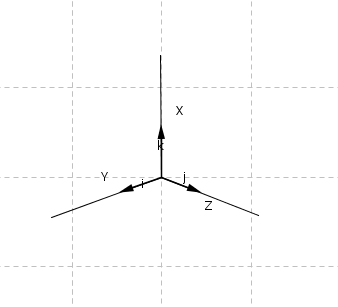
\includegraphics[scale=2]{figures/ijksystem.png}\\
\caption{Picture of a right handed 3-D coordinate system with ijk-basis-vectors on the axes pointing (imaginary)
into three dimensions. See \cite{Corral1} for introduction.}
\end{figure}

In this document we will design a $2 \times 3$ coordinate system for maps from the 3-D space onto the 2-D plane. We will generalize it to $m \times n$ additionaly. I will give practical examples 
because the $2 \times 3$ operator is very useful, making plotted vector-valued, respectivly multivariate, functions and their surfaces ready for the display on the 2-D computer screen. For simplicity, we draw in the examples with ES5 and ES6 JavaScript code onto the 2-D context of the HTML5 Canvas Element, without the need for WebGL, $4 \times 4$ matrices, and WebGLSL, by connecting the points in order of appearance with the lineTo(x,y) function. The new knowledge you obtain can be transferred onto afterwards.\\

I will give examples, how to use the 3-D coordinate system. I will explain, how it works, since we just sum up the horizontal parts of each axis multiplied by the corresponding coordinate of the input, to one final horizontal displacement of the resulting point. And we sum up the vertical amounts of each axism scaled with the coordinate of the same index from the input, for the final vertical displacement.

Since we let the third or n-m dimensions collapse, there may more than one point result in the same point in the target space. This is called compactness in my eyes, since we cover a point obtained earlier again with the result of another vector transformed. This is not a bad property. Do not think that. One of the main problems is just that of inverting the calculation. In the $n \times n$ case, you can divide the right side by T and use the inverse matrix. $Tx = y \Rightarrow^{:T} x = T^{-1}y$ To reconstruct the original in the $m \times n, m \lt n$ case, some informations are needed.


To reduce the n-m indeterminable variables of the unsolvable underdetermined system to a system of k equations in k unknowns, you need to know, what you can remove from the system and the results. This is different from function to function. But for example, explained with the $2 \times 3$: if you plot $z_i=f(x_i,y_i)$, on a square of x and y, and know the rectangle, you plot on, it is not a problem, to remove the $i*\Delta x$ or $i*\Delta y$ from the i-th coordinate vector and to solve the remaining 2x2 system. 

\subsection{Overview: What we will do in the document}

I will use this document, to explain the transformation, especially for the 2-D map, which is very useful for simple computer graphics and for example HTML5 Programmers needing a simple 3-D formula for simple 3-D graphics with the 2-D API of the Canvas.
Of course it can be used for OpenGL or XWindows, for 2-D Java, Windows, Android, iPhones and for any API, you can use to draw 2-D.
And on the other side, it is interesting mathematically, since the rectangular matrices and non-orthogonal bases are badly documented, following the main line of the lectures.


\begin{enumerate}
\item We choose angles for our axes relative to the x-axis. The axes can be rotated freely around the unit circle.
\item We choose a value for $r$. This is the length of one unit on each of the axes. It can be chosen freely.
\item We write down the three vectores derived from the canonical basis vectors $r(cos \theta, sin \theta)^{T}$ and apply our angles and lengths.
\item We assemble a matrix $\boldsymbol{A}$ with the axis vectors. And i will present a little of modern operator theory.
\item We read the example source code for a computer function, which is exactly two lines long. One line is for the new $x$-coordinate and one line of code is for the new $y$-coordinate.
\item We get the proofs for the linear behaviour of the transformation. And that 0 stays in 0. And a point on the axis on the axis.
\item We read other mathematical versions of the transformation. As a function, for example. And we will find connections between.
\item We derive the generic case of transforming n-coordinates down to the plane. 
\item We will derive the general $m\times n$ case by making use m-dimensional spherical coordinates for n axis in n-dimensional space.
\end{enumerate}\\



\begin{enumerate}
	\item The map is surjective
	\item The inverse function is not constructable, because the covered points are not seperable into their former domain coordinates. 
	\item Conditional reconstruction. With heuristic information, like knowing the x coordinates and the delta steps allows to reduce the 2x3 to a 2x2 after subtracting the known part.
\end{enumerate}

\textbf{Warning! Foreign author.}\\

Edward Gerhold, who is writing this document, is nativly speaking german. 

Maybe this text contains phrases, he understands, which no one, nativly speaking english, would be able to understand.\\
%\newchapter{1}


\subsection{Organisation of this document}

The revisions of this second draft of the promised content is organised into the following parts:

\begin{enumerate}
	\item Preliminaries
		All used definitions and theorems from linear algebra and 
		Glossary of my speech (coordinate system, axis, map, projection, transformation, )
		Notation

	\item Construction 
		About indexes
		
		Angles
		Unit length
		Sets of axes = basis for the map = operator in other words
		The operation
		- explaining the sum of scaled axes as the final point like entering it manually in a coordinate system by travelling parallel to the axes 

	\item Properties of the map, the functions, the matrices
	\item Corollaries Generalisation into m dimensions, coordinate functionals for components
		Four and more dimensions on the plane
		Generalisation into m dimensions
		Coordinate functionals,
		The self-adjoint matrices which result from multiplication with it´s own transposition
		Embedding into higher dimensions
	
	\item Experimental 
		- like gram schmidt on 2x3 which can not be made indy)

	\item Discussion
		- 
		-

	\item Example Source Code in form of a collection of JavaScript functions for the HTML5 Canvas 2-D Context
\end{enumerate}


\subsection{Mathematical prelimiaries}

Let us get quickly through a few definitions, lemmata and theorems, which we will use and exploit during our studies of my results about mapping $m \times n$ by my own words.

\begin{description}
	\item{Map} A map is the image of all points being transformed. It is the graph of the function or a transformed graph.
	\item{Linear map} A linear map is of class $C^1$ and a sum of coordinates times a basis-coefficient for each point.
	\item{Open set} An open set lies inside of a given closed interval, excluding the boundary points.
	\item{Closed set} The closed set includes the boundary
	\item{Boundary} For example is the boundary of a disc the circle outlining the disc for example $r*e^it$ is a circle with radius r around the origin of the complex plane, which is isomorphic to the $R^2$ plane and gives all points on the circle line for the boundary of the disc inside the circle line.
	\item{Function}
	\item{Functional}
	\item{Matrix}
	\item{Linear Operator}
	\item{Linearity} In a linear function you can substitute $b+c$ for $a$ and reveal for $A(a)$ then $A(b) + A(c)$, which is clearly a proportionally correct sum. In a nonlinear system the extra terms prove, $let A(a)$ be $A(a) := a^2$ that $A(b+c)$ is not equal to $A(a)$ because $A(b+c)$ is no longer $A(b)+A(c)$ but $A(b)+A(\sqrt 2 \sqrt b \sqrt c)+A(c)$.
	\item{Nonlinearity} 
	
	\item{k-Forms} Differential forms make multivariate calculus easier. In the first version i did not study them, meanwhile i am getting deeper into.

	\item{Coordinate System} A coordinate system in this document is the word for that kind of coordinate system, you know from drawing graphs of functions or points in the euclidean space. It has axes and integers with one unit distance on them. You enter points by going along each axis by the amount of the coordinate (component) which belongs to the axis.

	\item{$\cos \theta$ and $\sin \theta$} Irreplaceable functions, a vector on the plane can be split in it´s orthogonal parts in terms of cosine and sine times the length of our vector. This is used to give for each x,y,z the x and y amounts for moving along the plane and generalized to spherical coordinates




	\item{global coordinates} The $R^n$ points are the global sys

	\item{local coordinates} An object in $R^n$ given some center point has a local coordinate system, if from this center to the boundary the coordinates are counted. The coordinates in $R^n$ may differ by the distance from center to center and by the configuration of the coordinate calculation.
\end{description}


\subsubsection{Vector spaces}


We are dealing with vector spaces. The set of the coordinate axes is called the basis. 


The formula of the basis is the main formula we need to understand to understand how we sum scaled vectors. Exactly the axes which are scaled by the coordinates to represent the way each coordinate goes along the corresponding axis. The sum of the scaled axes is the point in the coordinate system. 

\subsubsection{Hamel basis}

There is the Hamel Basis Theorem. Every vector space has a basis.

hamel basis


There are fine properties for orthogonal bases, where all parts are independent and perpendicular.
In matrix form you have the eigenvalues and principal axes from the eigenvectors and can solve the linear system with the inverse matrix obtained by moving from the left hand side $Tx = y$ to the right hand side $x = T^{-1}y$. 


Orthogonal bases


But there is the space of $m \times n$ matrices, with $m \lt n$. This is my favorite space to discuss here. And the bases can not be completly independet. In my eyes it is time to let me introduce the term of the non-orthogonal or dependent basis, i could not call it the Gerhold Basis, which garantuess the correctness of the coordinate systems axes, even, when they collapse some dimensions. I will explain it mainly with the $2 \times 3$ system, but will generalize it to n axes with m dimensions.



\subsubsection{Metric space, normed space, inner product space}


We start with the definition of a metric $d(x,y) = \|x-y\|$ on a vector space. 



\begin{displaymath}
    d(\vec{x}, \vec{y}) = \|\vec{x}-\vec{y}\| = \sqrt{\sum_{i=1}^{n}|\vec{x}_{i}-\vec{y}_{i}|^2}
\end{displaymath}



This function turns the space $X$ into a metric t

Metrics have three fundamental properties.

\begin{enumerate}
\item $d(x,y) = 0 \iff x = y$ If the distance is zero, the vectors are equal.
\item $d(x,y) = d(y,x)$ It does not matter, whether you read $d(x,y)$ or $d(y,x)$, the number must be equal. The absolute value function $|\pm n| = n, \pm n \in \mathbb{R}$ makes sure
\item $d(x,z) \leq d(x,y) + d(y,z)$ The third one is the triangle inequality. Going over another point is always a step longer.
me\end{enumerate}

The type of vector space increases by the functional operations defined on the space.

To make a n-dimensional space measurable, first introduce the metric. Which measures the distance from x to y.


This is to be improved by introducing a norm on the space. The norm is used to measure the length of the vector or function. This makes them comparable.


\paragraph{Hausdorff property}

\newtheorem{hausdorff}{Definition. Hausdorff property.}
\begin{hausdorff}
A space has the Hausdorff property, if all points can be seperated by unit balls, which cover the whole space respectivly all points.
\end{hausdorff}

\subsubsection{coordinate system}

With the book "Vector Analysis versus Vector Calculus" i have seen the term coordinate system with new eyes, because it is written down as pair of a set and a map. 

A coordinate system is a pair of a set and a map $(S, \mu)$

The set $S$  is the set of all points in the coordinate system.

An the function $\mu$ maps all coordinates from the domain $S \subset D(\mu)$ to the range $R(\mu)$ of $\mu$.

\begin{displaymath}
	\mu : S \subset D(\mu) \rightarrow R(\mu)\\
	(x,y,z) \rightarrow (x\cos \varphi_x + z\cos\varphi_x, y\sin\varphi_y + z\sin \varphi_z)
\end{displaymath}



\subsubsection{My Notation: coordinate system for $m \times n$ maps}

In the $m \times n$ case with $m \neq n$ has the previous notation of a pair of set and map to be improved by
stating a domain set and a range set together with the map, since the map is mapping to some other space than itself.


I would like to call it $(D,R,\mu)$ consisting of the input domain, the output range, and the map function(s).


\subsubsection{My term: non-orthogonal basis}

\begin{definition}
	\item[map basis]
	\item[non-orthogonal]
	\item[]
\end{definition}


combined basis


collapsed basis
normalized basis
non orthogonal basis
general map basis
partially linearly dependent basis
surjective map basis
transformation basis
dimension collapsing basis



\newtheorem{coordsys}{Coordinate system}
\begin{coordsys}
\end{coordsys}

\newtheorem{axis}{Coordinate system}
\begin{axis}
\end{axis}





A $\mathbb{K}$-Vectorspace V over a body $\mathbb{K} = \mathbb{R}$ or $\mathbb{K} = \mathbb{C}$ is a set $V$ with the two operations $+$ and $\cdot$. In the example of our coordinae system we have set $\mathbb{K} = \mathbb{R}$. Written as ring it is written as $(V, +, \cdot)$. The vector space possesses two operations.

Addition: $+: V \times V \rightarrow V, (\vec{x},\vec{y}) \mapsto \vec{x}+\vec{y}$\\
Scalar multiplication: $\cdot: K \times V \rightarrow V, (\lambda, \vec{x}) \mapsto \lambda\vec{x}$.\\

A K vector space V must fulfill the following axioms.\\

\begin{enumerate}
\label{kvs_axioms}
\item $\forall \vec{a},\vec{b} \in V. \vec{a}+(\vec{b}+\vec{c}) = (\vec{a}+\vec{b})+\vec{c}$ (associativity)
\item $\forall \vec{a},\vec{a}' \in V. \vec{a} + \vec{a}' = 0 = \vec{a}' + \vec{a} \forall a \in V$ (additive inverse)
\item $\forall \vec{a} \in V. 1\vec{a} = \vec{a}$    (1 is an identity operator)
\item $\forall \vec{a},\vec{b} \in V.  \vec{a}+\vec{b}=\vec{b}+\vec{a}$ (commutativity)
\item $\exists \vec{0} \in V,\forall \vec{a} \in V. \vec{0}+\vec{a}=\vec{a}$ (zero element)
\item $\forall \lambda,\mu \in K, \forall \vec{a} \in V. \lambda(\mu\vec{a})=\lambda\mu\vec{a}=\mu(\lambda\vec{a})$ (scalar associativity)
\item $\forall \lambda,\mu \in K, \forall \vec{a} \in V. (\lambda + \mu)\vec{a} = \lambda\vec{a}+\mu\vec{a}$
\item $\forall \lambda \in K, \forall \vec{a}, \vec{b} \in V. \lambda(\vec{a}+\vec{b}) = \lambda\vec{a}+\lambda\vec{b}$  (distributive law)
\end{enumerate}



There are two kinds of norms. Norms of vectors of finite length, Emwhich are sums under the sigma signs. And norms of continuous functions, which are sums under the Integral sign. For the self-study, we will get a quick view onto function spaces, as well as for the continuous forms of our maps using functions instead of vectors representing fixed points in the basis spanned vector space.



The typical function spaces you will encounter are these. $C[a,b]$ is the space of continuous functions. It is seen as infinite dimensional. $C^k[a,b]$ is the space of k-times differentiable functions, whose first derivatives are in C^{k-1}, the second in C^{k-2}, and so so. There a variations of, like the C_0 containing all functions, integrals, sequences, with a limit of zero.

The norm on C is:
The inner product is:


'\begin{enumerate}
\label{common_function_spaces}
\item $C[a,b]$, space of all continuous functions on [a,b], infinite dimensional, integral norm, scalar product with complex conjugation
\item $L^p(R^n)$, spaces of lebesgue integrale functions, on some underlying space, integral norms, integral scalar product
\item
Em\end{enumerate}

Then there are unreplacable spaces of sequences, they are to be seen as complex spaces until otherwise stated, and have inner product with conjugation, and integral norms unless otherwise stated.

\begin{enumerate}
\label{common_function_spaces}
\item $C[a,b]$, space of all continuous functions on [a,b], infinite dimensional, integral norm, scalar product with complex conjugation
\item $L^p(R^n)$, spaces of lebesgue integrale functions, on some underlying space, integral norms, integral scalar product
\item
\end{enumerate}


Brings me to the notions of completeness and compactness.

I´ll try to give complete with my own words.

\newtheorem{Completeness}{Definition. Completeness of a vector space.}
\begin{Completeness}
A vector space, a function space, a sequence space is complete in it´s norm, if for any sequence $(x_n)_{n\in \mathbb{Z}}$ there is a finite subsequence $(x_{nk})$ which converges to a value x in the space. This means that $\|x_{nk}-x\| \rightarrow 0$ as $k \rightarrow \infty$ and we write $x_{nk}\rightarrow x$. A complete space is called a Banach space. For example, $\mathbb{R}^{n}, \mathbb{C}^{n}$ with $n\geq1$ are complete.
\end{Completeness}

And also give compact in my own words.

\newtheorem{Compactness}{Definition. Compactness.}
\begin{Compactness}
A space is compact on an interval, if there is a finite collection of subsets covering the space by their union. In terms of a compact operator there are more than one items from the domain which map to the same point on the range.
\end{Compactness}



\newtheorem{Covering Map}{Covering Map}
\begin{Covering Map}
A space is compact on an interval, if there is a finite collection of subsets covering the space by their union. In terms of a compact operator there are more than one items from the domain which map to the same point on the range.
\end{Covering Map}



Mapping? How can we map. I will try to give a 3-D coordinate system in 2-D. For this we will use fundamental mathematical tools.

\subsubsection{The dot products}


 \subsection{Dot product}

The dot product, scalar product or inner product.
It is the most important vector vector multiplication defined in space.
It makes calculations with angles and detection of orthogonality possible.\\

It is the sum of the vector component products with either itself, or another vector.\\

If you pull the square root out of the dot product with a vector and itself, you obtain the current length of the vector.
Dividing the vector by it`s length will normalize the vector to a length of $1$. $\|\vec{x}\| = 1$ is called the unit length.
The formula and proof of the normalization of a vector is in \ref{normalizing_a_vector}\\

$(\vec{x}, \vec{y})$ is $\sum_{i=1}^{n}\vec{x}_{i}\vec{y}_{i}$.  \\

$\sum_{i=1}^{n}\vec{x}_{i}\vec{y}_{i} = 0$ means, that $\vec{x} \perp \vec{y}$ \\

The basis formula is this

\begin{displaymath}
    (v,w) = \sum_{i=1}^{n}\vec{x}_{i}\vec{y}_{i}
\end{displaymath}

A product with the zero vector.

\begin{displaymath}
    (\vec{0},w) = \sum_{i=1}^{n}\vec{0}_{i}\vec{y}_{i} = 0
\end{displaymath}

Algebraic simplifications and linear combinations.

\begin{displaymath}
    (\lambda\vec{x},\vec{y}) = \sum_{i=1}^{n}\lambda\vec{x}_{i}\vec{y}_{i}
    = \lambda\sum_{i=1}^{n}\vec{x}_{i}\vec{y}_{i} = \lambda(\vec{x}, \vec{y})
\end{displaymath}

\begin{displaymath}
    (\lambda\vec{x},\vec{y}+\vec{x}) = \sum_{i=1}^{n}\lambda\vec{x}_{i}(\vec{y}_{i}+\vec{x}_{i})
    = \lambda(\sum_{i=1}^{n}\vec{x}_{i}\vec{y}_{i}+\sum_{i=1}^{n}\vec{x}_{i}\vec{x}_{i})
    = \lambda((\vec{x},\vec{y})+(\vec{x},\vec{x}))
\end{displaymath} 

\begin{displaymath}
    (\lambda\vec{x},\kappa\vec{y}) = \sum_{i=1}^{n}\lambda\vec{x}_{i}\kappa\vec{y}_{i}
    = \lambda\kappa\sum_{i=1}^{n}\vec{x}_{i}\vec{y}_{i} = \lambda\kappa(\vec{x}, \vec{y})
\end{displaymath}

\begin{displaymath}
\begin{center}
    (\lambda\vec{x}+\mu\vec{x},\kappa\vec{y}+\nu\vec{y})\\
    = \sum_{i=1}^{n}(\lambda\vec{x}_{i}+\mu\vec{x}_{i})(\kappa\vec{y}_{i}+\nu\vec{y}_{i})\\
    = (\lambda\vec{x},\kappa\vec{y}) + (\lambda\vec{x},\nu\vec{y}) + (\kappa\vec{y},\mu\vec{x}) + (\kappa\vec{y},\nu\vec{y})\\
    = \lambda(\kappa(\vec{x},\vec{y}) + \nu(\vec{x},\vec{y})) + \kappa(\mu(\vec{y},\vec{x}) + \nu(\vec{y},\vec{y}))\\
\end{center}    
\end{displaymath}




\begin{enumerate}
\item
\item
\end{enumerate}




For our main example, the 3-D onto 2-D map, we will have the euclidean vector spaces $\mathbb{R}^{3}$ and $\mathbb{R}^{2}$ as domain and range of our operator matrix and our vector valued function. TBecause the $\mathbb{R}^{n}$ spaces are their dual and bidual spaces itself, the coordinate functionals i will discuss are to be found here, too.




\subsubsection{Vector Normalisation}

Each axis vector being normalised to a length of $1$ is probably the most important property for constructing a concise non-orthogonal basis. You can not have full orthogonality, that all axes are perpendicular to all other axes.  The coordinate systems axes represent aso the length of one unit in the direction of the axis. Mathematical correctness without scaling factors is provided by the unit length of one, that means in terms of the norm $\|e_n\| = 1$. So i should remind you to use the normalisation formula.

\begin{displaymath}
    \vec{e}_{normalized} = \frac{\vec{e}}{\|\vec{e}\|} \implies \|\vec{e}_{normalized}\| = 1
\end{displaymath}


\label{normalizing_a_vector}

\newtheorem{Normalisation}{Normalisation of a vector}
\begin{Normalisation}
	To normalize a vector $\vec{e}$ with a length of $\|e\| = l$ to a normalised length of $\|e\|=1$, you have to multiply each component by $\|e\|^{-1}$ and divide the components by the old length. $\forall e_i, (i \in 1,...,m) \hat{e}_{i} = \frac{e_i}{\|e\|}$. The new vector \hat{e} has a unit length of one, and $\|\hat{e}\| = 1$. 
\end{Normalisation}

\textbf{Proof}:

\begin{displaymath}
\vec{y}  = \left(\begin{array}{1}a\\b\end{array}\right)
\end{displaymath}
\begin{displaymath}
    \|\left(\begin{array}{1}a\\b\end{array}\right)\| = \sqrt{a^{2}+b^{2}}\\
\end{displaymath}
\begin{displaymath}
    \vec{y}_{normalized} = \frac{\vec{y}}{\|\vec{y}\|} 
    = \left(\begin{array}{1}\frac{a}{\sqrt{a^{2}+b^{2}}}\\\frac{b}{\sqrt{a^{2}+b^{2}}}\end{array}\right)
\end{displaymath}
\begin{displaymath}
    \|\vec{y}_{normalized}\| = \sqrt{\left(\frac{a}{\sqrt{a^{2}+b^{2}}}\right)^{2}+\left(\frac{b}{\sqrt{a^{2}+b^{2}}}\right)^{2}} = \sqrt{\frac{a^{2}+b^{2}}{a^{2}+b^{2}}} = \sqrt{1} = 1
\end{displaymath}

This formula is irreplaceable, and is needed to construct correct axes for our coordinate system. Our bases, mainly $m \times n$ can not be completly orthogonal, that is the direction the axis points into. But we can set them to have the correct length of one unit. This gives correct results, like with orthonormal systems, when mapping points into the as well normalised coordinate system.

\subsubsection{An example where the importance of normalization is easy to observe}
\label{why_normalization}

Consider the Hilbert-Space $\mathbb{R}^{2}$ with the orthogonal projection formula $(\vec{x},\vec{e}_{i})\vec{e}_{i}$. It is first a scalar returned inside the parens. It is a dot product of our source vector and the basis vector. The scalar returned by the two is then multiplied again with the basis vector. This results in a new vector. But. This only works fine, if the basis vector is normalized.\\

\textbf{Example}

a) Unnormalized -wrong results-\\

\begin{displaymath}
\begin{align}
\vec{e}_{1} &= \begin{pmatrix}2\\0\end{pmatrix}\\
\vec{e}_{2} &= \begin{pmatrix}0\\2\end{pmatrix}\\
\vec{x} &= \begin{pmatrix}3\\2\end{pmatrix}\\
\sum_{i=1}^{2}(\vec{x},\vec{e}_i) = (3*2+2*0)*\vec{e}_{1} + (3*0+2*2)*\vec{e}_{2}\\ 
&= 6*\vec{e}_{1} + 4*\vec{e}_{2} = \begin{pmatrix}18\\12\end{pmatrix}\\
\end{align}
\end{displaymath}

You see, the vector gets twice enlarged by a factor of the basis vector. This is why the normalization is crucial for the formula  $(\vec{x},\vec{e}_{i})\vec{e}_{i}$.\\

b) Normalized -right results-\\

\begin{displaymath}
\begin{align}
\vec{e}_{1} &= \begin{pmatrix}1\\0\end{pmatrix}\\
\vec{e}_{2} &= \begin{pmatrix}0\\1\end{pmatrix}\\
\vec{x} &= \begin{pmatrix}3\\2\end{pmatrix}\\
\sum_{i=1}^{2}(\vec{x},\vec{e}_i) = (3*1+2*0)*\vec{e}_{1} + (3*0+2*1)*\vec{e}_{2}\\ 
&= 3*\vec{e}_{1} + 2*\vec{e}_{2} = \begin{pmatrix}3\\2\end{pmatrix}\\
\end{align}
\end{displaymath}


The thing is similar in my understanding in having the r-value set to anything other then $1$ for all axes. The difference is, that our formula here is not multiplying twice with each r each component like this formula $\sum^{i=1}^{n}(\vec{x}|\vec{e}_{i})\vec{e}_{i})$






\subsubsection{Orthogonalisation with Gram-Schmidt}

In a $n \times n$ system, with as many axes as components, full orthogonalisation of some existing coordinate system is possible. The Gram-Schmidt process starts with the first axis, normalizes it, and then continues with the second axis. The parts of the first axis are removed, then the second axis is normalised. From the third one you remove the linear combined parts of the first and the second axis. Then you normalise the new axis. The fourth axis removes the linear combinations of the previous three axes, then is normalised and so on. 
 
Of course, you can not fully orthogonalize any $m \times n$ system with $m \lt n$, because you have more axes than components and to combine at most $n-m$ axes with directions occupied by the m linear independent axes. But the process itself is also applicable on the $m \times n$ system. It returns a set of combined, but normalised axes.


The unusual experiment to apply the Gram-Schmidt iteration to the 2-D vectors, which can not be made independent, is following in the appendix under unusual experiments



\subsection{Orientation}

For integration of Curves, Surfaces, Manifolds, the notion of orientation is of primary importance. There is the notion of the outward normal vector and the inward normal vector for Curves, Surfaces, Manifolds. There is a notion for a positive (anticlockwise) and a negative (clockwise) orientation


\paragraph{Outward normal vector}



\paragraph{Inward normal vector}

This is the normal vector pointing to the inner side of the 


\paragraph{Negative Orientation}

Around the circle we go anticlockwise. 

\paragraph{Positive Orientation}

For example on the unit circle, we travel clockwise.




\newchapter{Construction of $m \times n$ coordinate systems}

\section{Designing a $\mathbb{R}^{2\times{3}}$ coordinate system for our transformation from $\mathbb{R}^{3}$ to $\mathbb{R}^{2}$}

This chapter deals with the construction of a $2 \times 3$ coordinate system. It is taking three coordinates and returning two coordinates. When using such a three dimensional coordinate system manually, you would go along the first axis for the value of the first coordinate, then continue parallel to the second axis with the length of the second coordinate, and then parallel to the third axis by the amount of the third coordinate. We do this mathematically and in a programming language and take a sum of the three vectors we just walked along by doing it manually and parallel to the axis. The sum or the final destination is our new point, which is the right coordinate on the plane inside a three-dimensional looking coordinate system.

First i will give a few words about notation and indices used throughout the text to make it easier for you, to follow my indices and letters.

\subsection{Notation: The $_{n}$ indices $_x,_y,_z$ with $_x=1$, $_y=2$ and $_z=3$ for the components equal as for the vectors $\vec{e}_n$}
\index{index}

The index $_{n}$ in $r_{n}$, $\varphi_{n}$, $\vec{e}_{n}$ is the index for $_x$,$_y$,$_z$. For example $\varphi_{n}$  stands $\varphi_x, \varphi_y, \varphi_z$. $r_{n}$ stands for $r_x$, $r_y$ and $r_z$. $\vec{e}_{n}$ is for $\vec{e}_x$, $\vec{e}_y$, $\vec{e}_z$ It is possible, that in the formulas $x,y,z$ and $1,2,3$ may be used interchangeably. For example, when summing up the products of the coordinate components with the basis components, this happens. The formula is $\sum_{i=1}^{3}\vec{x}_{i}\vec{e}_{i}$, which is a sum of $x,y,z$ and the $\cos \varphi_{n}$ terms in the first components of $\vec{e}_{n}$ for $x$ and a sum of $x,y,z$ and the $\sin \varphi_{n}$ terms in the seconds components of $\vec{e}_{n}$ for $y$.\\

Being on point explaining indices, i should also explain this. The coordinates $x,y,z$ in the vector $\vec{x}$ are the same as the components $\vec{x}_{1},\vec{x}_{2},\vec{x}_{3}$. And the components $x, y$ in $\vec{y}$ are equal to $\vec{y}_{1}, \vec{y}_{2}$.\\

Throughout the text vector x is the input vector, vector y is the output vector. x,y,z and x,y use the same letters for points in space and in the plane. While this text is a draft, i also may have used v,w for the vectors.

\textbf{Remark} Recently i have learned more about spaces, dual spaces, adjoints, function representations and can not say, that i will make it this version water-proof. But i will and can answer more open or unasked questions in the coming updates of this text.

\subsection{$\varphi_{n}$ the angles for the coordinate axes}

Each axis vector has an angle relative to the x-axis on the plane. This angle is measured to make use of the cosine and sine functions to return the horizontal and vertical amounts, the axis moves a coordinate, when multiplying the axis with the scalar of the coordinate component. The sum of all three horizontal parts is the new x coordinate on the plane and the sum of the vertical parts is the new y coordinate. Chosen as vectors we find coordinate functionals mapping from space to a single number, which is possible in all dimensions. How to create functionals for any $x_n$ component will be shown later.

\begin{figure}[ht]
\label{handsystems}

\includegraphics{figures/handsystems.png}
\caption{A right handed (z-up) and a left handed coordinate system. They just have different angles in our 2-D projection.}
\end{figure}

Whether the angles have to be measured in degrees or in radians, that depends on the cosine and sine functions you use.
In most cases it will be radians. You should be familiar with $\frac{\pi}{2} = 90^{°}$ and how to convert to degrees and back.
Cosine and sine should be introduced into the class of your best friends of all time mathematics because you will need them frequently and maybe just daily.

\fbox{We will arrange the three axes for x, y and z around the circle. By choosing an angle for each axis. In the $2 \times 3$ case we can use the circle. In higher dimensions, we will arrange them with spherical coordinates inside some m-dimensional sphere, with m-1 angles each axis, to let each of the axes point into the right directions.) }\\


Let the set of all $\varphi_{n}$ with $n \in {1, 2, ... }$ be the set of axis angles for axis $1$ to axis $n$. In higher dimensions we will have a set of angles $\varphi_{i,n}$ with $i \in {1, 2, ..., m-1}$ for each of the n axes. In the $2 \times 3$ mapping there exists one angle for each axis, mapping from higher dimension onto the 3-D sphere has 2 angles per axis (spherical coordinates). Higher dimensions generalize equal with more general spherical coordinates.\\

 I put the angles into a set in this document to simplify grouping and accessing the informations for applying the theorems. By using the subscript index $_{n}$ in numbers or letters, as $_x, _y, _z$ or $1,2,3$. $\varphi_x$ or $\varphi_1$ is the angle of the x-axis. $\varphi_y$ or $\varphi_2$ is the angle of the x-axis and $\varphi_z$ or $\varphi_3$ is the angle of the x-axis. \\

 In later generalizations i will use $\varphi_{i, n}$ which describes the i-th angle of the n-th axis. This sounds more complicated, but the generalized cosine and sine vectors in spherical coordinates provide the precisest configurability of all of these axes by providing for example the radius property to multiply with the length of the axis and the freedom of moving it freely around the m-dimensional manifold (sphere) we map onto. Remember that these generalized axes also have a unit norm of one $\|\vec{e}_n\| = 1$ or $\|\vec{e}_n\| = \rho_n$ if the unit factor (known as radius of circle and sphere) is set to a different value than 1.

\begin{displaymath}
\begin{align}
\varphi_{n} :=& \{\varphi_x, \varphi_y, \varphi_z\ | \varphi_n \mbox{are angles for the three 2-D axis vectors}\}\\
 =& \{ \varphi_1, \varphi_2, \varphi_3 | \varphi_n \mbox{are angles for the three 2-D axis vectors} \}
\end{align}
\end{displaymath}

I will show the notation for the set of angles for one m-dimensional axis. Each of the n axes in m dimensions has m-1 angles in general spherical coordinates which allow to configure the n m-dimensional axes precisely. Using the cosine and sine in m dimensions makes it possible to take the correct amounts for each axis slope componentwise.

\begin{displaymath}
\begin{align}
\varphi_{i,n} :=& \{\varphi_{1,x}, \varphi_{2,x}, ..., \varphi_{m-1, x}\ | \varphi_{i, n} \mbox{are a set of m-1 angles for the each of n m-dimensional axis vectors for on geralized spherical coordinate basing axis vectors}\}
\end{align}
\end{displaymath}

In the $2 \times 3$ case the angles are measured around a circle. In higher dimensions we measure the axes directions around a sphere in the corresponding dimensions of the range of the transformation (target dimension) with general spherical coordinates. This enables us to map precisly and to know where the axes point to. 

\subsubsection{Take the angles in degrees or radians?}

Maybe you have to convert the angles beetween degrees and radians. It depends on the cosine and sine functions, you use. For example, the JavaScript \emph{Math.cos($\varphi$)} and \emph{Math.sin($\varphi$)} functions take radians. Most other programming languages, like Java or C/C++ take radians, too. I will repeat this simple conversion now for you.

\begin{example}
\textbf{Definition 1}
The function rad converts degrees to radians, it´s useful for computer functions taking radians.
\begin{displaymath}
\text{rad}(\phi) := \frac{\pi}{180} \times \phi, \phi \in \mathbb{R}
\end{displaymath}

\textbf{Example 2}
\label{120_degrees}

Here is an example of three angles. The three axes have an angle of 120 degrees between each neighbour axis. We start counting from the horizontal x-axis counterclockwise with positive numbers in radians, or negative numbers, if we go clockwise. We have to add each angle 120 degrees, after choosing our first angle.\\
 
\begin{displaymath}
\varphi_x = \text{rad(210)}, \varphi_y = \text{rad(330)}, \varphi_z = \text{rad(90)}
\end{displaymath}

\begin{displaymath}
\varphi_x &= \frac{\pi}{180} \times 210 &= \frac{7\pi}{6},  
\varphi_y &= \frac{\pi}{180} \times 330 &= \frac{11\pi}{6}, 
\varphi_z &= \frac{\pi}{180} \times 90 &= \frac{\pi}{2} 
\end{displaymath}
\end{example}

\textbf{Definition 3}
The function deg converts conversely from radians to degrees. You multiply your value with the reciprocal of PI/180, namely 180/PI and get the opposite result of the rad function. This proves, that $deg(rad(x))=x$ and $rad(deg(x))=x$.\\

\begin{displaymath}
\text{deg}(\phi) := \frac{180}{\pi} \times \phi, \phi \in \mathbb{R}
\end{displaymath}

\textbf{Example 4}
The first example, Example 1, was about an a little bit rotated righthand coordinate system. Here are some angles for a lefthand system, which includes the third axis with exactly 45 degrees beetween the perpendicular x and y axis.\\

\begin{displaymath}
\varphi_x &= \frac{\pi}{180} \times 0 &= 0,  
\varphi_y &= \frac{\pi}{180} \times 90 &= \frac{\pi}{2}, 
\varphi_z &= \frac{\pi}{180} \times 45 &= \frac{\pi}{4} 
\end{displaymath}

If you would like to get hands on angles, cosines, sines, or need a refresher, \cite{Corral2} is a good choice. And as well \cite{Corral1} and \cite{Strang2} teach unit circles, polar coordinates, sines, cosines and wonderful mathematics.\\

\begin{figure}
\begin{tabular}{-l-l-l-l-l-l-}
Angle &     sin &   cos & tan & csc & sec & cot\\
$0^{\circ}$  &    $0$&  $1$&  $0$&  undefined&  $1$&  undefined\\
$30^{\circ}$ & $\frac12$ & $\frac{\sqrt{3}}{2}$ & $\frac{1}{\sqrt{3}}$ & $2$ & $\frac{2}{\sqrt{3}}$ & $\sqrt{3}$
$45^{\circ}$ & $$& $$& $$& $$& $$& $$\\
$60^{\circ}$ & $$& $$& $$& $$& $$& $$\\
$90^{\circ}$ & $$& $$& $$& $$& $$& $$\\
$120^{\circ}$ & $$& $$& $$& $$& $$& $$\\
$135^{\circ}$ & $$& $$& $$& $$& $$& $$\\
$150^{\circ}$ & $$& $$& $$& $$& $$& $$\\
$180^{\circ}$ & $$& $$& $$& $$& $$& $$\\
$210^{\circ}$ & $$& $$& $$& $$& $$& $$\\
$225^{\circ}$ & $$& $$& $$& $$& $$& $$\\
$240^{\circ}$ & $$& $$& $$& $$& $$& $$\\
$270^{\circ}$ & $$& $$& $$& $$& $$& $$\\
$300^{\circ}$ & $$& $$& $$& $$& $$& $$\\
$315^{\circ}$ & $$& $$& $$& $$& $$& $$\\
$330^{\circ}$ & $$& $$& $$& $$& $$& $$\\
\end{tabular}

\caption{Overview over the trigonometric function values. This table is written down from \cite{Corral2}.}
\end{figure}

\subsection{$r_{n}$ and $\rho_{n}$ are factor which describes a unit of one on each axis}

It is possible to choose another name for the unit length of a one on the axis. But to stay closely related to the basic operations i use to construct the axes with, namely the polar coordinate substitutions for x and y, giving a vector from the origin into the direction of the angle, with the length of the chosen factor, i keep the familiar letters of $r$ and in higher dimensions of $\rho$.

\begin{displaymath}
r_{n} := \{ r_{x}, r_{y}, r_{z} | r_n \mbox{ is the unit for $1$ on each axis }\} = \{ r_{1}, r_{2}, r_{3} | r_n \mbox { is the unit each axis } \}
\end{displaymath}

And in higher dimensions we will have no extra index, but i will use the letter of spherical coordinates, $\rho$.

\begin{displaymath}
\rho_{n} := \{ \rho_{u}, \rho_{w}, \rho_{x}, \rho_{y}, \rho_{z}, ... | \rho_n \mbox{ is the size of a one (one unit) on each of the n axes with m components.}\} = \{ \rho_{1}, \rho_{2}, \rho_{3}, \rho_{4}, \rho_{5}, ... | \rho_n \mbox { is the unit each axis } \}
\end{displaymath}

In my first draft i had already a little to mention about the r-value:

\begin{enumerate}
\item The axes have $\|\vec{e}_{n}\|_{2}=1$ if you set $r_x = r_y = r_z = 1$. This gives mathematical unchanged results.
\item If you set $(r_x = r_y = r_z) > 1$ you scale the image by that factor, if it is $(r_x = r_y = r_z) < 1$ you shrink the graph.
	The mathematical results get changed.
\item If you set all r-values to different lengths, rotation of objects inside the coordinate system look unrealistic. For that use a 		local basis for each object and set the coordinate system itself again to r-values equal on all axes.
\item If you the the r-values to different lengths than $1$, all mathematical results get changed and the whole examination is more 	  complicated, and maybe not solvable, since we got it to do with an non-invertible operator.
\end{enumerate}

In short $\|\vec{e}_{n}\| = r_n$, and the best option is, to set all three axes to normalized length of $1$.\\


 The coordinates can be scaled independently from the transformation by multiplying the 2-D points with a zoom factor, which can be $zoom > 1$ to enlarge, or $\frac{1}{z}$ to scale down. This factor can be applied by the drawing function after the point transformation.\\

 Of course is any kind of graphics processing before and after our process possible.

\fbox{The number $r$ is for the length of one unit on each axis. $r_x=r_y=r_z=1$ is optimal.}\\

\fbox{If you want to measure data you should stick with unit length of 1.}

\subsection{$\vec{e}_{n}$ describe the 1-n axes with m components for the non-orthogonal basis of the map}

We have drawn some axes on a piece of paper and taken the angles starting from zero counterclockwise on the x-axis.
We know now, that elonginating an axis vector by changing the radius forces us to draw one circle for each axis. You see the
unit ball with the diameter of $2$ and a radius of $1$ which is $r$. But visually it is not there, if you use the coordinate system.\\

Now we will write down the three basis vectors. Each vector points from the origin onto the circle line of its axis. With the same
values on alle axes, in the document we will use the unit length of $1$, they share the same circle on the first unit. And no matter how you rotate them, on all units. We will still map 3-D coordinates with three 2-D axes onto the 2-D screen.

Let $\vec{e}_{n}$ be the set of three two dimensional basis vectors. In this document and some literature and scripts,
we call them $\vec{e}_x$, $\vec{e}_y$ and $\vec{e}_z$. Another well known names for the basis vectors are $\vec{i}$, 
$\vec{j}$ or $\vec{k}$ for example. That is equal to the picture of the coordinate axes at \ref{ijksxstem} in this document.\\

Multiplying the 2x3 basis with the 3x1 points later results in wonderful 2x1 points. We will see it as a function, derivation of the derivatives and the integral over the e-vector function doing the coordinate transformation after upgrading by adding the coordinate by the rules of integration.\\

\begin{displaymath}
\vec{e}_{n} := \{\vec{e}_x, \vec{e}_y, \vec{e}_z | \vec{e}_{n} \mbox{are the coordinate axes} \} = \{\vec{e}_1, \vec{e}_2, \vec{e}_3  | \vec{e}_{n} \mbox{are the coordinate axes} \}\\
\end{displaymath} 

This is now a set of the three axis vectors. We give them the letter $e$ and a subscript for the coordinate component in the numeric order of $x=1, y=2, z=3$. To arrange these vectors we already got around the unit circle and layed them out there. To measure the angles, beginning on the horizontal coordinate axis or zero, until we reach the vector. The vectors point into the positive direction of the described axis.\\

\begin{figure}[ht]
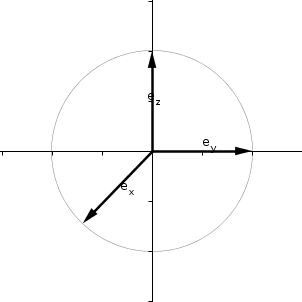
\includegraphics[scale=0.8]{figures/righthand45.png}
\caption{The three basis vectors point into the positive directions of the desired coordinate axes each. They are arranged around a circle with the trigonometric functions of cosine and sine. The coordinate system shown is a righthanded coordinate system.}
\end{figure}

\begin{figure}[ht]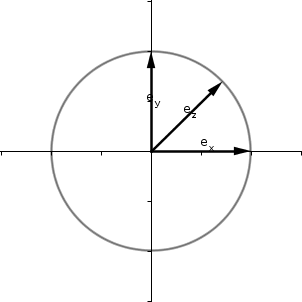
\includegraphics[scale=0.8]{figures/lefthand45.png}
\caption{The three two dimensional basis vectors as a lefthanded coordinate system.}
\end{figure}

To reach all three (x,y) at the tips of the vectors, we will now pull out the cosine and sine functions and stuff them together
with $r$ and $\varphi$ into a 2x1 vector with two components. So any (x,y) on one line from the origin to far distance can be reached like in polar coordinates\footnote{Interested readers may find in \cite{Corral1}, \cite{Corral2} and \cite{Strang2} everything about polar coordinates, parametrization of x and y with cosine and sine, the unit circle and the distance or radius r and more to these topics.} with the following parametrization.\\

\begin{displaymath}
\left(\begin{array}{1}x\\y\end{array}\right) = \left(\begin{array}{1}r \cos \varphi\\ r \sin \varphi\end{array}\right)\\
\end{displaymath}\\

Which can alternativly be written like $(x,y) = (r \cos \varphi, r \sin \varphi)$.\\

Modeling the three two dimensional basis vectors with this information,
we get the following three two dimensional basis vectors. They point along the coordinate axes and are the ruler for our transformation.\\

\begin{displaymath}
\vec{e}_x := (r_x\cos(\varphi_x), r_x\sin(\varphi_x) )^T = \left(\begin{array}{1}r_x\cos(\varphi_x)\\r_x\sin(\varphi_x) \end{array}\right)\\
\end{displaymath}
\begin{displaymath}
\vec{e}_y := (r_y\cos(\varphi_y), r_y\sin(\varphi_y) )^T = \left(\begin{array}{1}r_y\cos(\varphi_y)\\r_y\sin(\varphi_y) \end{array}\right)\\
\end{displaymath}
\begin{displaymath}
\vec{e}_z := (r_z\cos(\varphi_z), r_z\sin(\varphi_z) )^T = \left(\begin{array}{1}r_z\cos(\varphi_z)\\r_z\sin(\varphi_z) \end{array}\right)\\
\end{displaymath}\\

Each component of (x,y,z) has now it`s own basis vector. By multiplying the cos terms for the x and the sin terms for y with the corresponding component of (x,y,z) and summing the three products up for each of x and y, we directly obtain the right coordinate on the plane. All we would have to do is to connect the points again, or to fill the space between. \\

Remark. The basis is not orthogonal. My aim is to clear this field and to generalize the non-orthogonal Basis for $m \times n$ maps. Additionaly i will like to show the simple embedding of the map into any larger space, without restoring the collapsed dimensions.

\begin{figure}[ht]
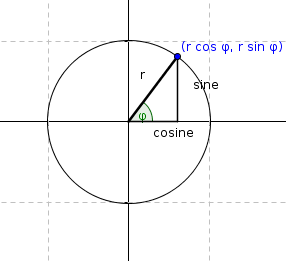
\includegraphics[scale=2]{figures/unitcircle.png}
\caption{A picture of the unit circle, the hypotenuse r, the adjacent cosine, the opposite sine and the angle $\varphi$. It is a circle of radius r, and no longer the unit circle, if $r \neq 1$.}
\end{figure}


The following definition is more difficult. The generalized axis vectors in spherical coordinates go like this

\begin{displaymath}
\vec{e}_{n} = \begin{pmatrix}
	\rho_n (\Pi_{i=1}^{m-1}\sin\varphi_{i,n})\\
	\rho_n (\Pi_{i=1}^{m-2}\sin\varphi_{i,n}) \cos \varphi_{m-1,n}\\
	\rho_n (\Pi_{i=1}^{m-3}\sin\varphi_{i,n}) \cos \varphi_{m-2,n}\\
	\vdots\\
	\rho_n \sin \varphi_{1,n} \cos \varphi_{2}\\
	\rho_n \cos \varphi_{1,n}\\
\end{pmatrix}
\end{displaymath}

Later i will show the $x_k$ coordinate functional taking the k-th component of each of the n of the m-dimensional axes and stick them together into one vector to dot them with the coordinate vectors. The $x_k$ coordinate functional live in the dual space of the n-dimensional domain of the attended transformation. But more about this later.\\

An example i give now is for a 3x4 matrix, to move 4 dimensions onto the 3-D sphere. We just need to angles for each of the four axes describing the directions and lengths of our basis vectors. To map from four dimensions onto three dimensions we need four of the three dimensional axes.

\begin{displaymath}
\vec{e}_{x} = \begin{pmatrix}
	\rho_x \sin\varphi_{1,x} \sin \varphi_{2,x})
	\rho_x \sin\varphi_{1,x} \cos \varphi_{2,x})
	\rho_x \cos\varphi_{1,x}
\end{pmatrix}
\vec{e}_{x} = \begin{pmatrix}
	\rho_x \sin\varphi_{1,y} \sin \varphi_{2,y})
	\rho_x \sin\varphi_{1,y} \cos \varphi_{2,y})
	\rho_x \cos\varphi_{1,y}
\end{pmatrix}
\vec{e}_{x} = \begin{pmatrix}
	\rho_x \sin\varphi_{1,z} \sin \varphi_{2,z})
	\rho_x \sin\varphi_{1,z} \cos \varphi_{2,z})
	\rho_x \cos\varphi_{1,z}
\end{pmatrix}
\vec{e}_{x} = \begin{pmatrix}
	\rho_x \sin\varphi_{1,t} \sin \varphi_{2,t})
	\rho_x \sin\varphi_{1,t} \cos \varphi_{2,t})
	\rho_x \cos\varphi_{1,t}
\end{pmatrix}
\end{displaymath}

They span the space of the four-dimensional coordinate system in three dimensional space. But they can not be completly orthogonal. For example you can let the x and the t axis use the same direction and over increasement of time, the points move to the right. Plotted at each instance of t you should see, how the thing moves to the right. But there is more about the physical interpretations concerning these axes as weights for the states in the vectors.


\subsection{Now we need the vector basis theorem}\\

\subsubsection{The general formula for importing a vector into a coordinate system}

We know how to multiply coordinates with a vector basis to get a new anticipated vector in the coordinate system the basis provides.

Or if we do not, we multply each coordinate component with it\'s corresponding axis and sum all scaled axis vectors together to a final vector. This is the goal matrix-vector multiplication achieves, when we transform for example graphics data the way we do.

The following theorem shows, how to sum up independent basis vectors  $(e_1, .., e_n)$ which are scaled by the individual coordinate component $(x_1, ..., x_n)$ to a final vector $x_1 e_1 + ... + x_n e_n$ containing the anticipated coordinates $(x_1, ..., x_n)$. 
The use of the non-orthogonal basis maps the correct images when mapping for example a three-d box on the 2-d plane.

\newtheorem{Vectorbasis}{Theorem. Hamel basis}
\begin{Vectorbasis}
A subset X of a linear vector space E is called a Hamel basis of E if every vector $x \in E$ can be uniquely expressed as a finite linear combination of some elements of X.
\begin{displaymath}
x=\sum_{k=1}^{n}a_{k}x_{k}
\end{displaymath}
for some nonzero scalar $a_{k}$ and vectors $x_{k} \in X$.
\end{Vectorbasis}
from \cite{Vershynin1}

My article broke in the first time, when i touched the rules of linear independent basis vectors, comparing them with my coordinate system. I have a set of dependent and independent vectors, because, for example, i have to move the z-coordinate into the x- and the y-coordinates, because i want to draw the three dimensions on a flat plane, shifting the x-y quotient spaces for each z into a direction. That direction is modeled by the axis vector.

I will explain it over and over throughout the text. Next to the linear independent set of basis vectors, which are common in 
$n \times n$ matrices, which can be orthogonalized by Gram-Schmidt, and consist of self chosen values or eigenvectors from 
calculated eigenvalues of a chosen matrix, which carries a set of axes for the n dimensions in the $n \times n$ matrix colums,
i will introduce a new term. Almost for myself it is new, and my own words.

After thinking for a while i think, it is right to coin the term of the non-orthogonal basis, which is synonymous for the set of n 
axis vectors with m components for $m \times n$ matrices.

\newtheorem{Non-orthogonal basis}{Definition. Non-orthogonal basis for $m\times n$ mapping. Caution! My own theorem.}

\begin{Non-orthogonal basis}
A non-orthogonal basis is a partially or completly linear dependent set of basis vectors. A non-orthogonal basis has more axes 
than components. In terms of a linear operator making use of the non-orthogonal basis is the dimension of the operators domain larger 
than the dimension of the operators range (the rank of the operator). The orthogonal construction of the basis is impossible because of the collapse of dimensions to map more axes onto a less dimensional surface. But correctly the set of vectors fulfill the same 
task as the orthogonal basis does in it´s domain. In their case the non-orthogonal basis provides a n-dimensional coordinate system on the m-dimensional space and units on the axes determined by the vectors lengths. The maps of a non-orthogonal basis are 
surjective. And because of the collapsed dimensions, points maybe covered by more than one input for a complete map of some set from the domain onto the range.
\begin{displaymath}
\end{displaymath}
\end{Non-orthogonal basis}

The next lemma is about the normalisation of the axes, to get a unit of $1$ long axis per column, meaning that $\|e_n\| = 1$. How to scale the axes, which will have it´s own applications, for example scaled display on a computer screen, or shrinking the axes dynamically for a perspective projection, will be pointed out during the text.

\newtheorem{normalized_axes}{Normalisation of the basis vectors}
\begin{normalized_axes}
The property of an axis-length of $\|e_n\| = 1$ defines one unit of a normalised axis. The relation to orthonormal basis is the same length of the axes, while the orthogonality property can be partially or nowhere fulfilled, normalisation is possible for all axes in the combined coordinate system.
\begin{displaymath}
\end{displaymath}
\end{normalized_axes}


Non-orthogonal basis is maybe not the best or only notion to describe the linearly combined set of axes. I will give a few more examples as a definition, that you may or may not use these words.

\newtheorem{new_basis_terms}{Definition. Combined, linearly combined, normalized, unit-long, partially orthogonal basis, dimension changing basis}
\begin{new_basis_terms}
Alternative names for the non-orthogonal basis. I propose the following. "Combined basis"  is pointing out, that some axes
are linearly dependent by combination of the existing directions. "Normalized basis" is pointing out, that the axes have the length of one, which is the mathematical property a well-defined non-orthogonal basis has. "Partially orthogonal basis", points out, that we use a couple of independent vectors for the basis and combine a few more, until the coordinate system we map into is ready for use.
\end{new_basis_terms}




\begin{figure}
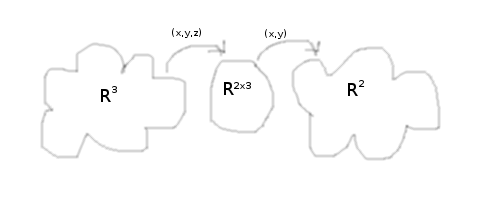
\includegraphics{figures/mediator.png}
\caption{A temporary picture of the process. We multiply the 3-D points with the 2x3 matrix and get the 2-D points back.}
\end{figure}

The point is, the general formula holds with a 2x3 basis.\\

\fbox{By taking 2-D vectors for three coordinates, we map directly onto the plane.}\\

\begin{figure}
\begin{displaymath}
    \boldsymbol{E}_{\mathbb{R}^2} = \begin{pmatrix}1 & 0 \\ 0 & 1\end{pmatrix}    \mbox{          }
    \boldsymbol{E}_{\mathbb{R}^3} = \begin{pmatrix}1 & 0 & 0\\ 0 & 1 & 0 \\ 0 & 0 & 1\end{pmatrix}    
    \boldsymbol{E}_{\mathbb{R}^{2\times3}} &= \begin{pmatrix}r_x\cos\varphi_x&r_y\cos\varphi_y&r_z\cos\varphi_z\\r_x\sin\varphi_x&r_y\sin\varphi_y&r_z\sin\varphi_z\end{pmatrix} \\
  \boldsymbol{E}_{\mathbb{R}^{2\times3}}_{225^{\circ}xrhs} = \begin{pmatrix}-\sqrt{\frac12}&1&0\\-\sqrt{\frac12}&0&1\end{pmatrix}     
\end{displaymath}

\caption{The standard basis for the $\mathbb{R}^{2}$ spans up the two dimensional space. When the three coordinates, which were a linear combination of $\lambda\begin{pmatrix}1\\0\\0\end{pmatrix} + \mu\begin{pmatrix}0\\1\\0\end{pmatrix} + \nu\begin{pmatrix}0\\0\\1\end{pmatrix}$ are combined into two coordinates, they become a linear combination of $\lambda\begin{pmatrix}1\\0\end{pmatrix}$ and $\mu\begin{pmatrix}0\\1\end{pmatrix}$. For sure, $\lambda$ is the sum of the cosine terms with the coordinates and $\mu$ is the sum of the sine terms with the coordinates in the two dimensions.}

\end{figure}

The formula for multiplying a vector with a basis to get a new vector is this. \footnote{The formula can be found in many mathematics, chemistry and physics lecture scripts, and a good introduction is \cite{Strang1}.}\\

\begin{displaymath}
\vec{y} = \displaystyle\sum_{i=1}^{n} \vec{x}_{i}\vec{e}_{i}
\end{displaymath}

This is the same formula for the linear combination in general.\\

It is done componentwise for each row of the vector. $n$ is the number of the source dimensions. In our case it is $n = 3$. 
We are summing three products for each component of the new vector. Our old $\vec{x}$ is a $\vec{x} \in \mathbb{R}^3$.\\
With $\vec{x}_{i}$ as the coordinate component and $\vec{e}_{i}$ as the corresponding basis vector in the right component. 
$\vec{y}$ is the resulting new vector.  The new vector $\vec{y}$ is a $\vec{y} \in \mathbb{R}^2$.\\

In our scenario is $V \subset \mathbb{R}^{3}, \vec{x} \in V$ and $W \subset \mathbb{R}^{2}, \vec{y} \in W$.\\

\subsubsection{Connection to ijk-Notation}

This is also equal to\\

\begin{displaymath}
\vec{x} = x\vec{i} + y\vec{j} + z\vec{k}
\end{displaymath}

what also explains, what the ijk-Notation means. If you don´t use it already for determining determinants for
calculating cross products (\ref{crossproducts}). It is for describing a vector. Don´t forget, our $i, j, k$ basis is two dimensional, 
because we draw on a 2-D plane like the computer screen or a piece of paper. \\

With a 3x3 basis the vector $x\vec{i} + y\vec{j} + z\vec{k}$ is equal to \left(\begin{array}{1}x\\y\\z'\end{array}\right)$. But with a 2x3 basis the vector $x\vec{i} + y\vec{j} + z\vec{k}$ is becoming  \left(\begin{array}{1}x\\y\end{array}\right)$\\

\subsubsection{Coordinate system}



\subsection{Time to show the operation}


The operation of multiplying the (x,y,z) coordinate with our $\mathbb{R}^{2\times{3}}$ coordinate axis vectors in order is the following:\\

\begin{displaymath}
\left(\begin{array}{1}x\\y\end{array}\right) = \left(\begin{array}{1}
xr_x\cos\varphi_x + yr_y\cos\varphi_y + zr_z\cos\varphi_z\\
xr_x\sin\varphi_x + yr_y\sin\varphi_y + zr_z\sin\varphi_z\end{array}\right)\\
\end{displaymath}\\

Right, this small formula brings over the $\mathbb{R}^{2\times{3}}$ the unexpected images of the preimage from $R^3$ to $R^2$.


Remark. Meanwhile i am ready to say $\mathbb{R}^{2\times{3}}$ image, and to believe, that this coordinate system is spanning the $\mathbb{R}^{2\times{3}}$ up (spread into the three dimensions) on the plane.\\


\newtheorem{span_2x3}{Proposition. The $2 \times 3$ matrix with the combined basis spans the triple-coordinate system on the plane}
\begin{span_2x3}
The $2 \times 3$ matrix with the combined basis spans the triple-coordinate system on the plane. It is not a span of linear independent axis, representing a vector space span of independent axes. But it takes three coordinates and maps them onto two coordinates, which are interpreted as two dimensional point or vector in the range of the operator. 
\end{span_2x3}


\newtheorem{2x3_isomorph_to_r2}{Proposition. The $2 \times 3$ space is isomorphic to real plane $\mathbb{R}^{2}$ respectivly the complex plane $\mathbb{C}$}
\begin{2x3_isomorph_to_r2}

\end{2x3_isomorph_to_r2}






\begin{figure}[ht]
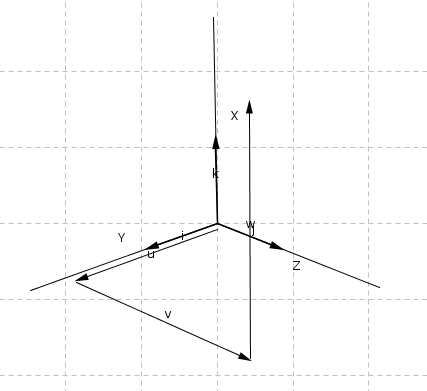
\includegraphics{figures/pathcoords.png}
\caption{The path a point goes from the origin. Along the first axis, then from that parallel to the second along that axis, and last parallel to the third axis as many units as the coordinate says. You can not see on this picture, how it is deconstructed by cosine and sine into left and right moves. To see, just draw the two missing sides of the triangles under each move. The z axis has a cosine of 0. I will paint a new picture for.}
\end{figure}\\

It is almost time to finish the matrix. And to go through a set of points. To draw the new set of resulting points.
For this i close the explaining chapters. And come to the part of the formal mathematical definitions. (Were i will
find alternatives for the matrix and related rules and laws, helpful for the understanding of the happenings.)\\

\textbf{Remark about the document structure.} \LaTeX and i are new to each other. For the theorems, proofs, defintions, corollaries, examples there is the possibility of a personal layout, which i have not prepared yet. And additionally, the following will contain some things, where real
mathematicians would start to smile. But i will do my best to correct any of my passages over the next time until i reach v1.0.0.\\


\newchapter{Practical transform tools: matrices, functions, notations, computer source code}

\section{The transformation $\mathbb{R}^{3} \rightarrow \mathbb{R}^{2}$ yields a perfect image}

\begin{figure}[ht]
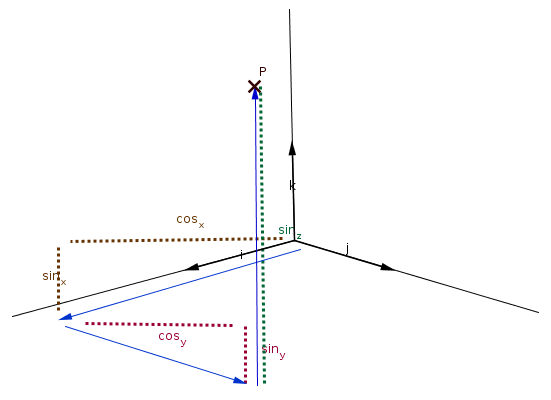
\includegraphics{figures/pathhacked.png}
\caption{The path a point goes from the origin. It is three moves horizontally and three vertically. One for each coordinate. Doing by scalar multiplication with the 2-D basis vector, all six proportional moves will be calculated, three of them build a weighted sum of a linear combination for interpretation of the $\mathbb{R}^{2}$ basis.}
\end{figure}\\

\subsection{Defining the Topology on the }

Remark. This subsection is started on July 31. And has still to be continued on Aug 20. Meanwhile i read a little of Munkres already and am fine, thanks.\\

Let $V$ be an open set in $\mathbb{R}^{3}$.\\

Let $B(\vec{x}, \epsilon)_{3}$ be a standard environment in the 3-space.\\

Let $W$ be an open set in $\mathbb{R}^{2}$.\\

Let $B(\vec{x}, \epsilon)_{2}$ be a standard environment in the 2-space.\\

Let the euclidean norm $\|\cdot\|_{2}$ be the default norm for three and two dimensions.\\

Let the $d(x,y)_{2} = \|x-y\|$ be the according metric.\\

Let $f:V\rightarrow W$ be a continuous function, and $A:V\rightarrow W$, $A \in L(V,W), Hom(V,W)$ be a rectangular matrix. Both map with equal operations V to W.\\

Let $V$ be the set of all points $(x,y,z) \in V \subset R^3$ which are about to become transformed. $V := \{ \vec{x}=(x,y,z)^T | x,y,z \in \mathbb{R}, \vec{x} \in V \subset \mathbb{R}^{3} \}$.\\

Let $W$ be the set of all points $(x,y) \in W \subset R^2$ which are the result of the transformation $W ;= \{ \vec{y}=(x,y)^T | \vec{y} \in W \subset \mathbb{R}^{2} x,y \in \mathbb{R}, \boldsymbol{A}\vec{x}=(x,y)^{T}\}$.\\

Remark. The topology has still to be defined extensivly in this document.\\



\subsection{Matrix version (Operator theoretic approach)}

A $m\times n$ matrix is a rectangle or square of numbers. Another name for the matrix is operator. In functional analysis operators can also be Integrals respectivly their kernel functions. A rectangular matrix like ours is a compact linear operator which is bounded. It is compact, because it is collapsing the dimensions, that results of vectors cover other results of other vectors with the same value.


A $n \times n$ matrix has nice properties. Determinants, Eigenvalues and Eigenvectors, an inverse matrix, which solves $Ax = b$ with $x = A^{-1}b$ (analogue to $ax = b$ with $x = a^{-1}b$ the matrix changes to it´s inverse element, when changing from the lefthandside to the righthandside). 

Our matrices will be rectangular. We will have more unknowns than equations. Or in my words we have a set of n axes with just m components.

\begin{displaymath}
    \boldsymbol{A} = (a_{ij})_{i,j \in \mathbb{N}^{+}} = \begin{pmatrix}a_{11} & ... & a_{1n}\\\vdots&\ddots&\vdots\\a_{m1} & ... & a_{mn}\end{pmatrix}
\end{displaymath}\\

Matrix with vector multiplication, from left to right in the matrix and from top to bottom in the vector, and that row by row, is achived by \\

\begin{displaymath}
    \boldsymbol{A}\vec{x} = (\sum_{j=1}^{n}a_{ij}\vec{x}_{j})_{i = 1..m} = \begin{pmatrix}a_{11}v_{1} + a_{12}v_{2} + ... + a_{1n}v_n\\\vdots \\a_{m1}v_{1} + a_{m2}v_{2} + ... + a_{mn}v_n\end{pmatrix} = \left(\begin{array}{1}w_{1}\\\vdots\\w_{m}\end{array}\right) = \vec{y}

\end{displaymath}\\

This formula is not much different from the multiplication with a vector basis, but it also accounts for the rows in the formula. The vector basis multiplication implies the componentwise row operations by using vectors.\\

\index{Definition}
\newtheorem{Definition}{Definition}
\begin{Definition}

Let \boldsymbol{A} be the matrix containing the three, two dimensional and trigonometric, basis vectors in order, one each
column. You get a rectangular 2x3 matrix $\boldsymbol{A} \in \mathbb{R}^{2\times{3}}: \mathbb{R}^{3} \rightarrow \mathbb{R}^{2}$. With the coordinate axis vectors $\left(\begin{array}{1}r_{n} \cos \varphi_{n}\\r_{n} \sin \varphi_{n}\end{array}\right)$ in the three columns. \\

\begin{displaymath}
\boldsymbol{A} := \begin{pmatrix}
    \vec{e}_x & \vec{e}_y & \vec{e}_z
    \end{pmatrix}
    = 
    \begin{pmatrix}
    r_x\cos(\varphi_x) & r_y\cos(\varphi_y) & r_z\cos(\varphi_z) \\
    r_x\sin(\varphi_x) & r_y\sin(\varphi_y) & r_z\sin(\varphi_z) \\
    \end{pmatrix}
\end{displaymath}\\
\end{Definition}


Remark. If $r_x = r_y = r_z$ you can pull out $r$ and write it in front of the matrix or multiply after transformation. A possible redefinition of the r-value is approaching. Remark of August 8.

%Remark. The operator definition should be defined differently.\\

%\newtheorem{DefinitionOperator}{Definition. A is a linear operator}
%\begin{DefinitionOperator}
%$\boldsymbol{A}$ is the linear operator $\boldsymbol{A} \in \mathbb{R}^{2\times{3}} : \mathbb{R}^3 \rightarrow \mathbb{R}^2$. This %operator maps coordinates from a subset of the $\mathbb{R}^{3}$ to the $\mathbb{R}^{2}$. ($\vec{x}) \mapsto \boldsymbol{A}\vec{x}$. 
%This operator is a matrix. But this operator is not invertible, because it is not square. It is not needed to be square, because we %map directly from the preimage to the image. The operator is mapping surjective, but since we interpret three dimensions on two, %there may be covered points on the plane, or overlaying of whole planes.
%\end{DefinitionOperator}\\

Remark. I commented the "linear map operator" definition out (linear map and operator is correct), because i have to write it again.


%Remark. About the matrix norm $\|A\|_{Frob}$. The number, after counting the components squares together and pulling the root is %$\sqrt{3}$. Pulling the norm chapter out of the introduction and introducing the measurements and estimations, also to myself, is %new on the TODO.


\index{Theorem}
\newtheorem{Theorem}{Proposition. My fundamental theorem of transforming 3-D Points into 2-D Points (Matrix)}
\begin{Theorem}
\label{Theorem}
If you multiply \boldsymbol{A}, the 2x3 matrix of the three two-dimensional basis vectors,
with the three-coordinate point $(x,y,z)$, the result is a two coordinate point, 
$(x,y)$. This point $(x,y)$ is the correct point on the two dimensional plane,
representing the point $(x,y,z)$ from the three dimensional coordinate system, you are transforming.\\
\begin{displaymath}
\boldsymbol{A}\left(\begin{array}{1}x\\y\\z\end{array}\right) = \left(\begin{array}{1}x\\y\end{array}\right)
\end{displaymath}

Applying the operator \boldsymbol{A} transforms the point $(x,y,z) \in V \subset \mathbb{R}^3$ into a new point $(x,y) \in W \subset \mathbb{R}^2$. 

\textbf{Proof}:\\

\begin{displaymath}
\boldsymbol{A}\left(\begin{array}{1}x\\y\\z\end{array}\right) = (\sum_{j=1}^{3}a_{ij}\vec{x}_{j})_{i=1,2}
%\end{displaymath}
%\beg{in{displaymath}
&= \left(\begin{array}{1}xr_x\cos(\varphi_x) + yr_y\cos(\varphi_y) + zr_z\cos(\varphi_z)\\
xr_x\sin(\varphi_x) + yr_y\sin(\varphi_y) + zr_z\sin(\varphi_z)\\
\end{array}\right) = \left(\begin{array}{1}x\\y\end{array}\right)
\end{displaymath}

\begin{figure}[ht]
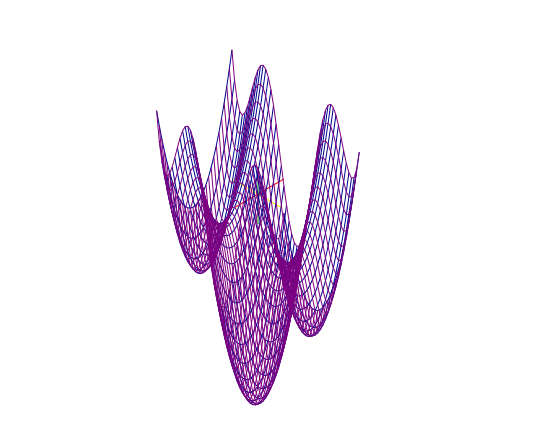
\includegraphics[scale=0.5]{figures/fxyplot.png}
\caption{$f(x,y) = x^2 + y^2 + 3y \sin y$ from [-5,5] and [-3,3] on a Canvas2DRenderingContext}
\end{figure}
\end{Theorem}


\subsection{Vectorbasis version}
\subsubsection{Hamelbasis with broken law of linear independence (or just a linear mapping)}

The theorem from Hamel says, that every vector space has a basis. And he gives a formula for this. The new vector in the new coordinate system is the sum of the coordinates multiplied with the basis vectors. \\

A Hamelbasis requires a linearly independent set of basis vectors. Which we can not provide. We change the dimension. The mapping yields the right image. So i will say, it is o.k. to break the rule of linear independence. This coordinate system is a special case.\\

\newtheorem{VectorBasisVersion}{Proposition. My fundamental theorem of transforming 3-D points into 2-D points (Vectorbasis)}
\begin{VectorBasisVersion}
If you multiply the three linear dependent two dimensional vectors with the three dimensional coordinates, they are mapped correctly onto the two dimensional coordinate system.
\end{VectorBasisVersion}

The operation is equal, but instead of working with three components in the new vector, we work with two components in the new vector. For each component, we build a sum of products. A sum of the productts of the basis components multiplied with the related coordinates ($x\vec{e}_x + y\vec{e}_y + z\vec{e}_z$), like we would do in the original form of this calculation with a $n\times n$ basis. \\

\begin{displaymath}
\vec{x} = \begin{pmatrix}x\\y\\z\end{pmatrix}
\end{displaymath}
\begin{displaymath}    
\vec{y} = x\vec{e}_{x} + y\vec{e}_{y} + z\vec{e}_{z}
\end{displaymath}    
\begin{displaymath}
    \sum_{i=1}^{n}\vec{x}_{i}\vec{e}_{i} = \left(\begin{array}{1}xr_x\cos(\varphi_x) + yr_y\cos(\varphi_y) + zr_z\cos(\varphi_z)\\
xr_x\sin(\varphi_x) + yr_y\sin(\varphi_y) + zr_z\sin(\varphi_z)\\
\end{array}\right) = \begin{pmatrix}x\\y\end{pmatrix} = \vec{y}
\end{displaymath}

The difference is that we have a dimension less than coordinates, and with that at least one axis, that must be a mix of the other two. By default our image in our coordinate system is a linear combination of $\lambda\begin{pmatrix}1\\0\end{pmatrix} + \mu\begin{pmatrix}0\\1\end{pmatrix}$, but before that, we map with a linear function from three dimensions to two dimensions, by using our coordinate system as or like a basis. \\

\newtheorem{VectorBasisBrokenLaw}{Proposition. Breaking the rule of linear independence to map from 3-D to 2-D}
\begin{VectorBasisBrokenLaw}
\label{broken_law_basis}
To transfer the points from 3-D to 2-D with the same formula, as mapping ordinary points with a vector basis into 
the corresponding coordinate system, it is o.k., to remove the third dimension from the basis and to multiply the
3-D coordinates with three 2-D vectors to get a correct mapping onto the projection plane.
\end{VectorBasisBrokenLaw}

\subsubsection{ijk-Notation Version}

The ijk-Notation is well known from describing vectors, from calculating cross products over determinants, from coordinate systems showing the normalized ijk vectors along the axes. The formula is this\\

\begin{center}
 $\vec{y} = x\vec{e}_{x}+y\vec{e}_{y}+z\vec{e}_{z}$
\end{center}

This is a very natural way. This is a real sum. The coordinates x,y,z multiply each a basis vector. This is the ordinary constant or scalar multiplication. Then the three scaled vectors are summed up together. This gives us a new vector, the sum of the three vectors. I have explained this already earlier, you can use this notation for this purpose, now it is time to repeat it. For a picture, look at figures \ref{ijksystem} and \ref{handsystems}.\\

\newtheorem{ijkVersion}{Proposition. The fundamental theorem of transforming 3-D points into 2-D points (ijk-Notation)}
\begin{ijkVersion}
If you write the vector down in ijk-Notation using the three two dimensional axis vectors, instead of three three dimensional linear independent basis vectors, the sum of the products with ijk and the coordinates, which is a new vector, equals the right vector on the 2-D plane.
\end{ijkVersion}

\textbf{Proof:}\\
\begin{displaymath}
 x\vec{e}_{x}+y\vec{e}_{y}+z\vec{e}_{z} = x\begin{pmatrix}r_x\cos\varphi_x\\r_x\sin\varphi_x\end{pmatrix} + y\begin{pmatrix}r_y\cos\varphi_y\\r_y\sin\varphi_y\end{pmatrix} + z\begin{pmatrix}r_z\cos\varphi_z\\r_z\sin\varphi_z\end{pmatrix} = \sum_{i=1}^{3}\vec{e}_{i}\vec{x}_{i} = \vec{y} = \begin{pmatrix}x\\y\end{pmatrix}
\end{displaymath}


\subsection{ijk-Basis replaced with 2x3 hyperbolic cosh, sinh}

The hyperbolic cosine and sine can be defined in terms of the exponential function.

\begin{displaymath}
\begin{align}
	cosh(\theta) &= \frac{\exp{\theta} + \exp{-\theta}}{2}\\
	*
	sinh(\theta) &= \frac{\exp{\theta} - \exp{-\theta}}{2}
\end{align}
\end{displaymath}


Time for an experiment. What happens, if we replace cos and sin with their hyperbolic pendant? I have good and bad news. The bad news first. I have to continue my studies and can bring the hyperbolic geometry now.

 

The good, i can draw 3-D on the 2-D canvas with, too.



\subsection{Function variant}

A bare function containing the summarization of the coordinatewise scaled axis vector can be composed with other functions having their range in the same domain and also with all kinds of functions having their domain equal to the range of our bare function.\\

\subsubsection{The linear vector valued function $f(\vec{x})$}

The vector valued function which maps from 3-D space to the 2-D plane should be standard in todays school lectures, since
the computer is absolutly all-day and a standard tool for pupils, teachers, for research and simulation. My simple formula
for a 3-D map on the 2-D plane allows pupils to plot surfaces by connecting the points with lineTo functions on the 2-D canvas
with just two lines of code for transforming the $(x,y,z)$ 3-tuple into the $(u,v)$ 2-tuple. To make it simple i will repeat how
the horizontal parts of the axis vectors are scaled by the corresponding coordinate component and that the sum of these horizontal parts of the scaled vectors give the y coordinate and the sum of the scaled vertical or scaled sine parts make the new y coordinate.
It is so simple, that any school should be about this formula, because it enables kids to do 3-D on the PC before learning the OpenGL and other modern accelerated 3-D programming libraries, which are complicated for the novice, and to much for just a plot of a few lines of a surface.

We begin with $\vec{f}(\vec{x}) : X \subset \mathbb{R}^{3} \rightarrow Y \subset \mathbb{R}^{2}$. 

By the basics of the functional analysis, we can figure out, that each $\vec{f}_{n} : \mathbb{R}^{3*} \rightarrow \mathbb{R}$ is a linear functional from the dual space mapping by multiplying the n-th component of each axis in order with each component in $\vec{x}$to obtain the projection of the coordinate vector onto a new n-th component $\vec{\hat{x}}_n$

Our vector valued function is a combination of all linear functionals. They do the map from any vector from the domain of the input vectors. For each target coordinate component, from 1 to n, there is $\vec{f}_{n}$ the corresponding partial function, which combines the input vector with the n-th component of the target axes, for the n-th component of a resulting vector (point, state) in the target space.

In the $2 \times 3$ example is 
$\vec{f}(\vec{x})$ mapping the three dimensional coordinates into our planar coordinate system. The multiplication of the components with the horizontal ($r_n \cos \varphi_n$) and vertical displacements ($r_n \sin \varphi_n$), which are the representation Assume we have the angles and units designed and the function is well defined for its purpose.\\

\begin{displaymath}
\label{f_function}
\begin{align}
\vec{f}(\vec{x}) :&= \left(\begin{array}{1}\vec{x}_{1}r_x\cos\varphi_x + \vec{x}_{2}r_y\cos\varphi_y + \vec{x}_{3}r_z\cos\varphi_z\\					\vec{x}_{1}r_x\sin\varphi_x + \vec{x}_{2}r_y\sin\varphi_y + \vec{x}_{3}r_z\sin\varphi_z\end{array}\right)\\			
\end{align}
\end{displaymath}

This can even be written more convenient. The interested reader might find the books by Michael Corrall \cite{Corral1} and Gilbert Strang \cite{Strang2} useful and is invited to use any kind of course material for studying vector calculus and linear algebra. \\

\begin{displaymath}
\begin{align}
			\vec{f}(\vec{x}) = \vec{x}_{1}\begin{pmatrix}r_x\cos\varphi_x\\r_x\sin\varphi_x\end{pmatrix} + \vec{x}_{2}\begin{pmatrix}r_y\cos\varphi_y\\r_y\sin\varphi_y\end{pmatrix} + \vec{x}_{3}\begin{pmatrix}r_z\cos\varphi_x\\r_z\sin\varphi_z\end{pmatrix}
	\end{align}
\end{displaymath}

\subsubsection{The adjoint function to \vec{f}(\vec{x}) is a map from 2 to 3} 

This is applying the two transposed vectors to a three-d vector. Analogue to the adjoint $3 \times 2$ matrix i will show in the section about the matrix formulation.\\



\begin{displaymath}
\begin{align}
			\vec{f}(\vec{x}) = \vec{x}_{1}\begin{pmatrix}r_x\cos\varphi_x\\r_y\cos\varphi_y\\r_z\cos\varphi_z\end{pmatrix} + \vec{x}_{2}\begin{pmatrix}r_x\sin\varphi_x\\r_y\sin\varphi_y\\r_z\sin\varphi_z\end{pmatrix} 
	\end{align}
\end{displaymath}



\newtheorem{FunctionVersion}{Proposition. My fundamental theorem of transforming 3-D points into 2-D points (Function))}
\begin{FunctionVersion}
The linear function (map) $\vec{f}(\vec{x})$ maps the points correctly from 3-D to 2-D. It is continuous in every point, the zero vector maps onto the zero vector. Passing a vector with three coordinates to the function results in a vector with two coordinates, which are the right coordinates on the 2-D screen.
\end{FunctionVersion}


\subsubsection{Composition of the functions $f \circ g$}

There are various possibilities to combine the output of g and the input of f. 
The extension combining the output of f with the input of h is the other possibility.

The following functions are compositions of two functions and take some input and return our 2-D points.
f is transformingthe vector returned by g. g is taking the input in all examples and f is reworking the coordinates.
In other words, f is the same function as previously shown in \ref{f_function}.\\

\textbf{Example 1}\\

A call to $g(t)$ is returning a vector $\vec{x}$ passed to $f(\vec{x})$ by using the composition $f \circ g$ :  $f(g(t)) = \vec{y}$\\

\begin{displaymath}
\label{g_of_t_code}
g(t) := \left(\begin{array}{1}t\cos t\\t\sin t\\t\end{array}\right)
\end{displaymath}
Becomes the following
\begin{displaymath}
\begin{align}
			(\vec{f}\circ g)(t) := \cos t\begin{pmatrix}r_x\cos\varphi_x\\r_x\sin\varphi_x\end{pmatrix} + t \sin t\begin{pmatrix}r_y\cos\varphi_y\\r_y\sin\varphi_y\end{pmatrix} + t\begin{pmatrix}r_z\cos\varphi_x\\r_z\sin\varphi_z\end{pmatrix}
	\end{align}
\end{displaymath}

This is a 2-D image of a conical helix. You can look at Figure 14 how this looks like from $0$ to a few rounds of $2\pi$.\\

\begin{figure}
\label{g_of_t_figure}
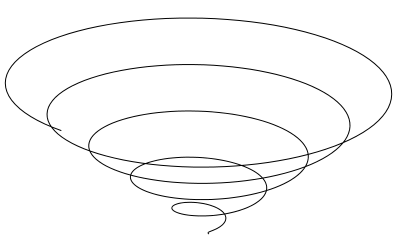
\includegraphics[scale=0.5]{figures/conicalhelix2.png}
\caption{This is $g(t)$ from \ref{g_of_t_code} in implement.html where implement.js from the repository is used once.}
\end{figure}

\textbf{Example 2}\\

 $g(x,y)=(x,y,z)$ this function will give us a surface plot. See figure \ref{g_of_x_y_figure}.\\

\begin{displaymath}
\label{g_of_x_y_code}
g(x,y) := \left(\begin{array}{1}x\\y\\e^{-x^{2} - y^{2}}\end{array}\right)
\end{displaymath}

That will be brought by $\vec{f}(\vec{x})$ into the following context. A function $(\vec{f}\circ g)(x,y) : E\times E \rightarrow W$.\\

\begin{displaymath}
\begin{align}
			(\vec{f}\circ g)(x,y) := x\begin{pmatrix}r_x\cos\varphi_x\\r_x\sin\varphi_x\end{pmatrix} + y\begin{pmatrix}r_y\cos\varphi_y\\r_y\sin\varphi_y\end{pmatrix} + e^{-x^{2}-y^{2}}\begin{pmatrix}r_z\cos\varphi_x\\r_z\sin\varphi_z\end{pmatrix}
	\end{align}
\end{displaymath}


\begin{figure}
\label{g_of_x_y_figure}
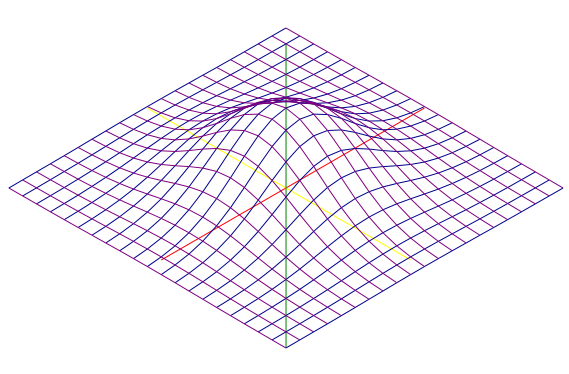
\includegraphics[scale=0.5]{figures/expfunction.png}
\caption{This is $\exp -x^{2}-y{2}$ from \ref{g_of_x_y_code} plotted with the cheap3danimate.html code within $[-2,2] \times [-2,2]$.}
\end{figure}

\textbf{Example 3}\\

A $g(x,y,z)$ or $g(\vec{x})$ a three-d or vector-valued function returning a three-d vector.\\

\begin{displaymath}
\label{g_of_x_y_z_code}
g(x,y,z) := \left(\begin{array}{1}x+1\\y\\z-1\end{array}\right)
\end{displaymath}

Which will become this kind of function. $(\vec{f}\circ g)(x,y,z) : E\times E \times E \rightarrow W$.\\

\begin{displaymath}
\begin{align}
			(\vec{f}\circ g)(x,y,z) := (x+1)\begin{pmatrix}r_x\cos\varphi_x\\r_x\sin\varphi_x\end{pmatrix} + (y)\begin{pmatrix}r_y\cos\varphi_y\\r_y\sin\varphi_y\end{pmatrix} + (z-1)\begin{pmatrix}r_z\cos\varphi_x\\r_z\sin\varphi_z\end{pmatrix}
	\end{align}
\end{displaymath}


The vector field of this formula is shown in figure \ref{vector_field_image}.

\begin{figure}
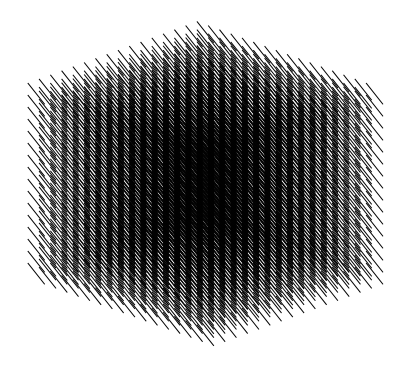
\includegraphics[scale=0.5]{figures/vectorfield.png}
\label{vector_field_image}
\caption{A 3-D vector field of a cubic section, this time of some random formula.}
\end{figure}

Remark. The vector field demo is primitive at this point.

\begin{center}
$g(\vec{x}) : \mathbb{R}^{3} \rightarrow \mathbb{R}^{3}$\\
$f(\vec{x}) : \mathbb{R}^{3} \rightarrow \mathbb{R}^{2}$\\
\end{center}


Remark. This section is not finished. Not only the plot for the vector field, some sophisticated demo with a physics formula, but the compositions are themselves not explained. Additionally in the section about differentiation, the compositions have to be veryfied.\\

\subsubsection{Vector valued function}
\label{vector_valued_func}

The book \cite{Corral1} defines a vector valued function like this:
\begin{displaymath}
f(t) = f_{1}(t)\vec{i}+f_{2}(t)\vec{j}+f_{3}(t)\vec{k}
\end{displaymath}

In our version this becomes a direct transformation onto the 2-D plane by using our 2x3 basis instead of a 3x3 basis.

\begin{displaymath}
f(t) = x(t)\begin{pmatrix}\cos\varphi_x\\\sin\varphi_x\end{pmatrix}
        +y(t)\begin{pmatrix}\cos\varphi_y\\\sin\varphi_y\end{pmatrix}
        +z(t)\begin{pmatrix}\cos\varphi_z\\\sin\varphi_z\end{pmatrix}
\end{displaymath}

Remark. The first chapter about differentiation, which follows later, deals with the constant form of $x(t), y(t), z(t)$. In a future version i will continue this topic with a few parametrized examples.\\



\subsubsection{The implicit mapping theorem for $\mathbb{R}^{3} \rightarrow \mathbb{R}^{2}$ from vector calculus}

I am proud of my formula, because i can not really find it anywhere in the lectures. A related mapping theory from
vector calculus is the "Implicit mapping theorem".

First we take the two gradients of $f_1$ and $f_2$.

The first one has the cosine parts of the function after taking the limit against zero to obtain the derivative.


\begin{displaymath}
\begin{align}
	\nabla\vec{f}_{1} = \begin{pmatrix}r_x \cos \varphi_x\\r_y \cos \varphi_y\\r_z \cos \varphi_z \end{pmatrix}
\end{align}
\end{displaymath}

The second one has the sine parts together in one gradient vector.

\begin{displaymath}
\begin{align}
	\nabla\vec{f}_{2} = \begin{pmatrix}r_x \sin \varphi_x\\r_y \sin \varphi_y\\r_z \sin \varphi_z \end{pmatrix}
\end{align}
\end{displaymath}



For the implicit mapping theorem for $2 \times 3$ functions we take the cross product of the two gradient vectors in 3-space.

\begin{displaymath}
\begin{align}
	\nabla\vec{f}_{1} \cross \nabla\vec{f}_{2} = \begin{vmatrix}i&j&k\\
	\partial_{x}f_{1}&\partial_{y}f_{1}&\partial_{z}f_{1}\\
	\partial_{x}f_{2}&\partial_{y}f_{2}&\partial_{z}f_{2}\\
	\end{vmatrix} = (-2^{-\frac12}, -2^{-\frac12}, 1)
\end{align}
\end{displaymath}



A suprise is to use these vectors in 3-space as a basis, putting them into the columns of a 3x3 matrix, to represent the axes of the 3-space, which we use to move by summing the scaled axes, scaled by the coordinates, to a final vector, the sum of the scaled axes, which is equal to moving along the first axis by the first coordinate, then moving parallel to the second axis with the second coordinate, and so on.

\begin{displaymath}
	\begin{pmatrix}\nabla f_1 \nabla f_2 \nabla f_1 \cross \nabla f_ \end{pmatrix} = \begin{pmatrix}
		1&0&-2^{-\frac12}\\
		0&1&-2^{-\frac12}\\
		2^{-\frac12}&2^{-\frac12}&1
	\end{pmatrix}

\end{displaymath}


Compared to the self-adjoint 3x3 matrix $A^{T}A$, we see that the cross product axis is just having reversed signs in $x_1, x_2$. I have not further examples, to compare with a general assumption, how close the implicit mapping theorem and the transpose product of axes, are related.

\begin{displaymath}
\begin{vmatrix}
	A^{T}A = \begin{pmatrix}
		1&0&2^{-\frac12}\\
		0&1&2^{-\frac12}\\
		2^{-\frac12}&2^{-\frac12}&1
	\end{pmatrix}
\end{vmatrix}
\end{displaymath}

The difference is just the sign of the cross product vectors compared to the self-adjoint product with the transpose. The cross product vector is orthogonal to the two gradient vectors. I have not researched further, to compare with the suspicious looking numeric relation.




Remark about $2^{\frac12}$. Remember some values. $\cos \varphi_z = \cos \frac{\pi}{4} = \cos 45^{\circ} = 2^{-\frac12} = \sqrt{\frac12} = \frac{1}{\sqrt{2}}$. This is the horizontal piece of a 45 degree z-axis pointing beetween perpendicular $(1,0)$ and $(0,1)$ x, respectivly y, axes right up. The sine value for forty-five degrees or a quarter of pi is identical with  $\sin \varphi_z = \sin \frac{\pi}{4} = \sin 45^{\circ} = 2^{-\frac12} = \sqrt{\frac12} = \frac{1}{\sqrt{2}}$. One of my favorised simplified coordinate system is the direct embedding of the z-axis half-half beetweeen the orthogonal planar basis.

\begin{displaymath}
\begin{align}
	A = \begin{pmatrix}
	1&0&2^{-\frac12}\\
	0&1&2^{-\frac12}
	\end{pmatrix}
\end{align}
\end{displaymath}

Remark. I must add a figure right to showing the unit circle and three vectors $e_x = (1,0)$, $e_y = (0,1)$ and $e_z = (2^{-\frac12}, 2^{-\frac12})$, to show the column picture (see Strang). The $e_n$ are in the columns and represent the axes of the coordinate system, respectivly the basis of the vector space. An open question for myself is, is this $2 \times 3$ space just the space of the operators carrying the axes? Or is the image it creates, which is isomorphic with the $\mathbb{R}^{2}$ Interpretation, beloning to the $2\times 3$ space. We would access a point with three coordinates, and read it off with two coordinates? In the last draft i was about to define the $2 \times 3$ plane as the plane with three coordinates. How clean can we describe this? Until then we map onto the euclidean plane from the euclidean space.





\subsection{Polar coordinate version}
\label{polar_coord_func}

The function can be written as a sum of three polar coordinate functions. The generic function for one component is this.

\begin{displaymath}
p(x, r, \theta) := xr\begin{pmatrix}\cos\theta\\\sin\theta\end{pmatrix}
\end{displaymath}

The sum of the three vectors gives us our correct position vector again.

\begin{displaymath}
P(x,y,z,r_x,r_y,r_z,\theta_x,\theta_y,\theta_z) :=  P(\vec{x}, \vec{r}, \vec{\theta}) := p(x, r_x, \theta_x)+p(y, r_y, \theta_y)+p(z, r_z, \theta_z)\\
\end{displaymath}

Well, i think this is ugly. And i should reconsider the r-value. Assuming the r-value be the usual normal unit length of 1, the functions become the following:

\begin{displaymath}
p_{n}(r, \theta) := r\begin{pmatrix}\cos\theta\\\sin\theta\end{pmatrix}
\end{displaymath}

And the whole combined function is again a sum of the three resulting 2-D vectors of the polar coordinate function.

\begin{displaymath}
P(\vec{x}) := p_{x}(x_{1}, \theta_{x}) + p_{y}(\vec{x}_{2}, \theta_{y}) + p_{z}(\vec{x}_{3}, \theta_{z})
\end{displaymath}



\subsection{The Coordinate-Functionals for x and y}

Sometimes you search for a tree in a forest, but can not find it, because the other trees look so similar like the tree you look for. 
This is the case for dot products, linear functionals from the dual space of the real space, and what i call the coordinate functionals.

I claim to have a well-defined tool to generate any coordinate component from any domain in any range from the first to the last vector component.

In our main example, the 3-D coordinate system for the plane, we use two coordinate functionals

\newtheorem{Coordinate_Functional}{Definition. Coordinate functional}
\begin{Coordinate_Functional}
A coordinate functional is a functional which returns, when applied to a vector from the domain it originates, a 
\end{Coordinate_Functional}





The cosine vector can be interpreted as linear functional from the dual space of the three dimensional euclidean space. Using the dot product to combine the functional with the coordinate vector maps to a real or complex value. In our case it is real and is equal to the new x coordinate for the plane. For this reason i call it the x-coordinate functional. It is to be defined on the dual space of the 3-D space and $\mathbb{R}^{3}$ is a space which is dual to itself, so it is to be found in $\mathbb{R}^{3}$. Dotting it with the three-d vector gives us the new x coordinate combined by combining the horizontal amounts of the axes expressed in terms of cosine.

\newtheorem{Definition}{The x coordinate functional for $R^{3} \rightarrow R^{2}$}
\begin{Definition}
The vector $(r_x \cos \varphi_x, r_y \cos \varphi_y, r_z \cos \varphi_z)$ is a linear functional on ${\mathbb{R}^{3}}^{\*}$. It contains the horizontal amounts of the three axes. Applying it onto a vector \vec{x} from \mathbb{R}^{3} results in the new x coordinate.
\end{Definition}

Analog is the y coordinate functional which carries the sine terms and the vertical amounts of the target axes.

\subsection{Computer implementations of the transformation}
\subsubsection{Generic computer code (all you need)}

One of the \emph{main goals of this document} is to show the simplicity of transforming 3-D points into 2-D points for the use in small computer applications. For example for hand written small web applications. Say, you just want to draw a graph, 3-D on the 
2-D Canvas and do not have the need for WebGL, or it is not available on your old target systems, which was the reason for me, to try it myself anyways.\\

This should be in a border box.\\

\begin{example}
\fbox{
The following is example code for various computer systems.
}
\begin{lstlisting}
x_ = x*r*cos(alpha) + y*r*cos(beta) + z*r*cos(gamma)
y_ = x*r*sin(alpha) + y*r*sin(beta) + z*r*sin(gamma)
\end{lstlisting}\\
\fbox{ These are the one and only two lines of code you need.\\}

\end{example}\\

\newtheorem{CodeTheorem}{Only two lines of code needed to go from 3-D to 2-D points. (Computer Version)}
\begin{CodeTheorem}
The only two lines of code you need to convert the coordinates on the computer. The new x value
is summed up by multiplying each coordinate with the cosine term of the related axis vector. The new y value
is a sum of products of the coordinates with the sine terms of the related axis vectors.
\end{CodeTheorem}

\subsubsection{JavaScript computer code}
\begin{example}
This is a full EcmaScript 6 snippet with all neccessary informations.\\
\begin{lstlisting}
let rad = (deg) => Math.PI/180*deg;
let r_x = 1, r_y = 1, r_z = 1; 
let phi_x = rad(220), phi_y = rad(330), phi_z = rad(90); 
let xAxisCos = r_x*Math.cos(phi_x), 
    yAxisCos = r_y*Math.cos(phi_y),
    zAxisCos = r_z*Math.cos(phi_z),
    xAxisSin = r_x*Math.sin(phi_x), 
    yAxisSin = r_y*Math.sin(phi_y),
    zAxisSin = r_z*Math.sin(phi_z);
let transform2d = ([x,y,z]) => [
    x*xAxisCos+ y*yAxisCos+ z*zAxisCos,
    x*xAxisSin+ y*yAxisSin+ z*zAxisSin];
let transform2dAll = (P) => P.map(transform2d);

let examplePoints = transform2dAll([[1,2,3], [3,4,5], [14,24,15]]);
\end{lstlisting}
\end{example}\\
\fbox{ This is the realistic amount of code to write to transform all points from 3-D to 2-D.\\}

\begin{figure}[ht]
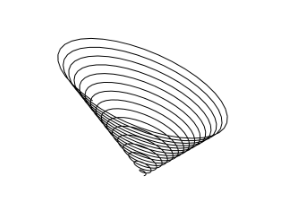
\includegraphics[scale=0.5]{figures/conicalhelix.png}
\caption{A conical helix (t/2*Math.cos(t), t*Math.sin(t), t) shown as (x,y,z)=f(t) with implement.html on a Canvas2DRenderingContext testing the javascript example code.}
\end{figure}

\section{Important proofs of the transformation behaviour}
\label{important_proofs}

A very important thing is to show, that the linearity of the transformation is in order. With a wrong function, bad thing can happen.
With the right functions, linear combinations should stay in the subspace.

\subsection{The origin stays in the origin}

A trivial proof is to prove, that the zero vector $\vec{0} \in \mathbb{R}^3$ maps to the zero vector $\vec{0} \in \mathbb{R}^2$.\\

\textbf{Proof}:
\begin{displaymath}
    \boldsymbol{A}\left(\begin{array}{1}0\\0\\0\end{array}\right)
    = \left(\begin{array}{1}0 + 0 + 0\\0 + 0 + 0\end{array}\right) 
    =\left(\begin{array}{1}0\\0\end{array}\right)
\end{displaymath}\\

\subsection{Points along one axis}

Another trivial proof is to prove, that coordinates lying on one axis are a multiple of the basis vector of the axis.\\

\textbf{Proof}:
\begin{displaymath}
    \boldsymbol{A}\left(\begin{array}{1}a\\0\\0\end{array}\right)
    = \left(\begin{array}{1}ar_x\cos \varphi_x + 0 + 0\\ar_x\sin \varphi_x  + 0 + 0\end{array}\right) 
    = a\vec{e}_x
\end{displaymath}

\begin{displaymath}
    \boldsymbol{A}\left(\begin{array}{1}0\\1\\0\end{array}\right)
    = \left(\begin{array}{1}0 + r_y\cos \varphi_y + 0\\0 + r_y\sin \varphi_y + 0\end{array}\right) 
    = \vec{e}_y
\end{displaymath}

\begin{displaymath}
    \boldsymbol{A}\left(\begin{array}{1}0\\0\\-b\end{array}\right)
    = \left(\begin{array}{1}0 + 0 - br_z\cos \varphi_z\\0 + 0 - br_z\sin \varphi_z\end{array}\right) 
    = -b\vec{e}_z
\end{displaymath}\\

\subsection{Multiplications with constants}

Another trivial proof is to show, that $\boldsymbol{A}(\lambda\vec{x}) = \lambda\boldsymbol{A}\vec{x}$. It doesn´t matter, where you multiply with the constant. You can multiply the original vector, or the resulting vector. You reach the same point.\\

\textbf{Proof}:\\
\begin{displaymath}
\begin{equation*}
\begin{align*}
\boldsymbol{A}(\lambda\vec{x}) &= \boldsymbol{A}\left(\begin{array}{1}\lambda{x}\\\lambda{y}\\\lambda{z}\end{array}\right)\\ &= \left(\begin{array}{1}\lambda{x}r_x\cos(\varphi_x) + \lambda{y}r_y\cos(\varphi_y) + \lambda{z}r_z\cos(\varphi_z)\\
\lambda{x}r_x\sin(\varphi_x) + \lambda{y}r_y\sin(\varphi_y) + \lambda{z}r_z\sin(\varphi_z)
\end{array}\right)\\
    &= \lambda\left(\begin{array}{1}xr_x\cos(\varphi_x) + yr_y\cos(\varphi_y) + zr_z\cos(\varphi_z)\\
xr_x\sin(\varphi_x) + yr_y\sin(\varphi_y) + zr_z\sin(\varphi_z)\\
\end{array}\right)\\
    &= \lambda\left(\begin{array}{1}x\\y\end{array}\right)\\
    &= \lambda\boldsymbol{A}\vec{x}
\end{align*}
\end{equation*}
\end{displaymath}\\


\subsection{Additions and subtractions}

Another trivial proof is to show, that $\boldsymbol{A}(\vec{x} + \vec{y}) = \boldsymbol{A}\vec{x} + \boldsymbol{A}\vec{y}$. 
It does not matter, if you add the original or the results . The outcome is the same point, the same vector.\\
 
\textbf{Proof}:\\

\begin{displaymath}
\begin{equation*}
\begin{align*}
\boldsymbol{A}\left(\begin{array}{1}x+u\\y+v\\z+w\end{array}\right) &= \left(\begin{array}{1}(x+u)r_x\cos(\varphi_x) + (y+v)r_y\cos(\varphi_y) + (z+w)r_z\cos(\varphi_z)\\
(x+u)r_x\sin(\varphi_x) + (y+v)r_y\sin(\varphi_y) + (z+w)r_z\sin(\varphi_z)\\
\end{array}\right)\\
            &= \left(\begin{array}{1}xr_x\cos(\varphi_x) + yr_y\cos(\varphi_y) + zr_z\cos(\varphi_z)\\
xr_x\sin(\varphi_x) + yr_y\sin(\varphi_y) + zr_z\sin(\varphi_z)\\
\end{array}\right) + \left(\begin{array}{1}ur_x\cos(\varphi_x) + vr_y\cos(\varphi_y) + wr_z\cos(\varphi_z)\\
ur_x\sin(\varphi_x) + vr_y\sin(\varphi_y) + wr_z\sin(\varphi_z)\\
\end{array}\right)\\    
    &= \left(\begin{array}{1}x\\y\end{array}\right) + \left(\begin{array}{1}u'\\v'\end{array}\right)\\
    &= \boldsymbol{A}\left(\begin{array}{1}x\\y\\z\end{array}\right) + \boldsymbol{A}\left(\begin{array}{1}u\\v\\w\end{array}\right)
\end{align*}
\end{equation*}
\end{displaymath}
\subsection{Rule of linearity}

\textbf{Corollary} From the previous two proofs, it is obvious to see, that
\begin{displaymath}
\boldsymbol{A}(\lambda\vec{x} + \kappa\vec{y}) = \lambda\boldsymbol{A}\vec{x} + \kappa\boldsymbol{A}\vec{y} = \lambda\left(\begin{array}{1}x\\y\end{array}\right) + \kappa\left(\begin{array}{1}u'\\v'\end{array}\right)\\
\end{displaymath}
which is a standard formulation of the rule of linearity. For example, you can find this rule in the form $\boldsymbol{A}(c\vec{x} + d\vec{y}) = c\boldsymbol{A}\vec{x} + d\boldsymbol{A}\vec{y}$ in \cite{Strang1}, but also in every linear algebra 1 lecture script.\\


\newchapter{Generalisations and corollaries, mapping and embedding theorems}


\section{Corollaries}


\subsection{Partial summary of properties we got or got not}

\begin{description}
	\item{No bijection} The map is surjective, if we collapse the dimensions. There exists no unique inverse map, only with additional informations, like reducing one of the coordinates by knowing the input numbers, the system can be changed into a solvable system. The surjective map means, it converts all points correctly into a linear combination, which yields the same image we would expect, or in other words, the surjection property is the right mapping property for the $m \lt n$ operator.
	
	\item{No inverse map} Only bijective maps have inverse operators, the injective property, which is missing is meaning a one-to-one assignment. The surjective construction is one, which combined two or more components into one and that in a way, which is not separable without additional help (like knowing one of the components over the whole line to remove them from the system to solve a determined one afterwards. For example $f(x,y)=z$ plots with $(x,y,f(x,y))$ can be restored if you know x and delta x and the number of points you plotted, that you can subtract them before.

	\item{No eigenvalues} Only square matrices have inverses, and only bijective mapping operators have eigenvalues not changing during the mapping. Eigenvalues and eigenvectors, which span the eigenspace for each eigenvalue are very useful and handy for
	solving systems of differential equations. How far this surjective operator (onto, and one way only since it collapses more than one dimension into one or more dimensions by combining the numbers and shifting the points a bit with) can be exploited for solving differential equations (i think of some images on mirrors, which are 2-D or on window glasses or similar 2-D images which appear in the real world naturally, but have not constructed or solved such yet)? I do not know today.


\end{description}

\subsection{$2 \times n$. Mapping to the plane}

\subsubsection{First Draft. Converting four Dimensions down to two dimensions}\\

The proposed theorem can be used to handle more dimensions, for example can four two-dimensional
vectors represent a 4-D space on the 2-D plane. They get converted into the correct
2-D points by giving each dimension a direction vector around the unit circle and relying the
horizontal and vertical amounts of cosine and sine. For Example, if you use a 2x4 matrix 
and convert all points at each instance of $t$ you have a moving object into the direction 
of the fourth basis vector. \\

\begin{displaymath}
\boldsymbol{A} := \begin{pmatrix}
    \vec{e}_x & \vec{e}_y & \vec{e}_z & \vec{e}_t\end{pmatrix}\\ = 
    \begin{pmatrix}
    r_x\cos(\varphi_x) & r_y\cos(\varphi_y) & r_z\cos(\varphi_z) & r_t\cos(\varphi_t)\\
    r_x\sin(\varphi_x) & r_y\sin(\varphi_y) & r_z\sin(\varphi_z) & r_t\sin(\varphi_t)\\
    \end{pmatrix}
\end{displaymath}

Here the basis is four times of two dimensions. A 2x4 matrix with four two dimensional basis vectors, one for each axis.\\

\begin{displaymath}
\boldsymbol{A}\left(\begin{array}{1}x\\y\\z\\t\end{array}\right) = \sum_{n} \vec{e}_{n}\vec{x}_{n} = \left(\begin{array}{1}x\\y\end{array}\right)\\
\end{displaymath}

\textbf{Proof}:

\begin{displaymath}
\boldsymbol{A}\left(\begin{array}{1}x\\y\\z\\t\end{array}\right) &= \left(\begin{array}{1}
xr_x\cos(\varphi_x) + yr_y\cos(\varphi_y) + zr_z\cos(\varphi_z) + zr_t\cos(\varphi_t)\\
xr_x\sin(\varphi_x) + yr_y\sin(\varphi_y) + zr_z\sin(\varphi_z)+ zr_t\sin(\varphi_t)\end{array}\right)\\
\end{displaymath}
\begin{displaymath}
&= x\vec{e}_x + y\vec{e}_y + z\vec{e}_z + t\vec{e}_t &= \sum_{n} \vec{e}_{n}\vec{x}_{n} &= \left(\begin{array}{1}x\\y\end{array}\right)
\end{displaymath}\\

The same method can be used, to convert points or vectors from any other number of dimensions, down to the $xy$-plane. 
It can so be used in a general $m \times n$ case, where one goes from $n$ dimensions down to $m$ dimensions.\footnote{http://de.wikipedia.org/wiki/Abbildungsmatrix, shows the m by n case.} 


\subsection{$m \times n$ - the great m by n mapping theorem or my generalisation of the $2 \times 3$ example.}

Let us get m-dimensional. And more complicated, when we use the formal way. Before that, i will show an easy way
to construct the $m \times n$ matrix.

We add up to m orthogonal axes.

We add the remaining n-m axes as linear combinaion with $\|e_n\| = 1$ or $\| e_n \| = r_n$ into the desired coordinate system. You may choose a suitable directions. If you have an application for, you will almost have the direction already together with the need.

This is the easy way.



The difficult and formal way, which describes also the whole $m \times n$ vector space for each matrix in the related form, is to use m-dimensional spherical coordinates, which is the natural extension to the polar coordinates, and means to have m-1 angles per axis for orientation in the m dimensions of the target, and to have n axes, which means to obtain n(m-1) angles to have a formal and componentwise orthogonal axis, which is completly described in terms of flexible m-dimensional sperical coordinates. 

The formula can describe any number in the vector space, so it is the general formula for constructing the axes for a $m \times n$ map.

To repeat it again. It is ok, to use $(0,1,0,0,... )$ for m axes and to insert the remaining m-n axes with combinations of norm one.

\subsection{Offline. Explaining the Fouriercoeffients with the $2 \times 3$ model.}

I care for Fourier transforms. By recently repeating the material i have got, i noticed it. Remember, the n-th coefficient is calculated by multiplying $f(t)$ with $e^{-int}$ (or in other letters, like in physics $e^{-ikx}$ and other representations are common), for around the circle, or along some interval. There is a constant term like $\frac{1}{2\pi}$ in front, being the modulus. I do not explain that now, as i think about the same when thinking about replacing the integral by another sum formula. But that is not what i want to state.

$e^{-int}$ is the same as $\begin{pmatrix}\cos nt\\-\sin nt\end{pmatrix}$. When multiplying with f(t) in terms of the integral, we go around the circle. Each infinitesimal t (we integrate with respect to t) we multiply the exponential with f(t). In our model it is the same as multiplying one axis vector $e^{-int}$ with a coordinate vector component $f(t)$. The integral sums this up. In terms of our coordinate system, we build the final sum, and the final point. This is on the complex plane. And if the coefficient is real, the result is to be found on the real axis. And if it is complex, you find it as one point on the plane. It can be calculated off the origin with polar coordinates and be seen as one point. 

cI think when we go round the circl e and multiply with f(t) the sum tells us the proportions the function has to any direction, the opposite side removes the amount from the opposite side if their sign is equal.

\subsection{Integral functionals explained for simplifying your efforts in getting the notion}


The integral functions differ from the discrete functionals in the number of components. The function in the integrand map to a real or complex number. We multiply for each infinitesimal element with a kernel function and sum the resulting numbers up to a final number. The difference in the vector product and the Integral of two functions multiplying is that we do not take componentwise products to sum up, but call instead the two functions each infinitesimal element. It is like an infinite series, which has or has no limit in the finite range. If it has a limit, the result is a real or complex number. The process itself of summing products up is closely related to the inner products summed up in the vector language. I hope this helps to get a clue more about what these continuous functionals are.

\newtheorem{cont_func}{Definition. Continuous functionals, Integrals}
\begin{cont_func}
Integrals, on finite and infinite vector spaces, are the continuous form of the vector valued functionals in terms of dot products.The sums of a basis vector, the integral kernel, and scaling factor, the function to multiply with, are almost equal, but continuous, and a sum of infinitesimal elements.
\end{cont_func}

Proof:

First i give an example as the limit of a Riemann-Sum, without taking the infimum of the upper sum and the supremum of the lower sum and to compare their equality. I will just let you look at the terms to combine, that you set the infinitesimal dot product as integral.

\begin{displaymath}
\begin{align}
	T_{k}f(x) &= \int_{a}^{b}f(t)k(x,t)dt\\
	&= \lim_{n \rightarrow \infty} \sum_{t=0}^{\infty} f(a + t((b-a)/n)) k(x, a+t((b-a)/n))) (b-a)/n
\end{align}
\end{displaymath}

I think you can conclude from this Riemann sum, that this is formally almost equal to a $\sum_{i=0}^{n} a_i e_i$. 


In terms of a Lebesgueintegral it is also a infite sum of products.

\begin{displaymath}
\begin{align}
	T(f, x) &= \int_{a}^{b}f(t)k(x,t)dt\\
	&= \lim_{n \rightarrow \infty} \sum_{t=0}^{\infty} f(a + t((b-a)/n)) k(x, a+t((b-a)/n))) (b-a)/n
\end{align}
\end{displaymath}


\subsection{A $scale(A,B)$ componentwise scaling function for matrices}


\subsection{A triangulation algorithm for $f(x,y)=z$ for drawing plots on a canvas}

\subsubsection{Taking the points}
\subsubsection{Drawing the points}
\subsubsection{Filling and lightning}



\subsection{The coordinate functionals}

\subsubsection{Functional analysis as motivation}

We come to one of the section i am proud of. I figured out, how to formulate the coordinates in terms of linear functionals. Since last year, i found the functional analysis interesting, because it was about metric, normed spaces, about sums of vectors and basis vectors, dot products and functionals mapping vectors to a number, like the scalar product and the norm, or well known integrals, like from calculus of variations, physics, or partial differential equations with functional analytic techniques. It was about matrices and operators, covered the spectrum i finally get used to, which is much simpler, than enqueueing it for a while, until we reach the topic.

I figured out, that the component wise definition of the maps is the same as the formulation in functionals from the dual space of the domain into the real or complex field by taking the coordinates and the functionals, dotting them and getting the component of the final point.

This brings me to the notion of coordinate functionals for each of the vector components.


\subsubsection{* From the first draft: Alternative definition of the transformation by using dot products}
\label{alternative_def_using_dot}
Underways, i came to another conclusion. If i pull the two row vectors out of the matrix and define them as two column vectors,
then i can dot each with the coordinate vector and write the dot product into the component of the resulting vector.\\

\begin{displaymath}
    \vec{x} = \left(\begin{array}{1}x\\y\\z\end{array}\right)       \vec{c} = \left(\begin{array}{1}r_x\cos\varphi_x\\r_y\cos\varphi_y\\r_z\cos\varphi_z\end{array}\right)            \vec{s} = \left(\begin{array}{1}r_x\sin\varphi_x\\r_y\sin\varphi_y\\r_z\sin\varphi_z\end{array}\right)
\end{displaymath}
 
\begin{displaymath}
    \vec{y} = \left(\begin{array}{1}\vec{x}\cdot\vec{c}\\\vec{x}\cdot\vec{s}\end{array}\right)
\end{displaymath}

The result is $\vec{y} \in W$, $W \subset R^2$.\\

This operation can also be extended into any finite number of dimensions, and will result in two coordinates then. Just add the dimensions to $\vec{x}, \vec{c}, \vec{s}$ and see.\\

\textbf{Proof}:

\begin{displaymath}
\left(\begin{array}{1}\vec{x}\cdot\vec{c}\\\vec{x}\cdot\vec{s}\end{array}\right) = \left(\begin{array}{1}
xr_x\cos(\varphi_x) + yr_y\cos(\varphi_y) + zr_z\cos(\varphi_z)\\
xr_x\sin(\varphi_x) + yr_y\sin(\varphi_y) + zr_z\sin(\varphi_z)\end{array}\right) = \left(\begin{array}{1}x\\y\end{array}\right)
\end{displaymath}


Meanwhile it is clear, that this operation is the same as $\nabla\vec{f}(\vec{x}) \cdot \vec{x}$, which is the natural dot product of the gradient vector of our linear function $\vec{f}(\vec{x})$ with the coordinate vector.


\subsubsection{The coordinate functionals}

I guess i will take a few definitions, lemmata and theorems until it is ready for you.

\newtheorem{coordinatefunctional}{Definition. Coordinate functionals}
\begin{coordinatefunctional}
A coordinate functional is a functional from the dual space of the domain resulting, when combined with any input vector from the domain, in a coordinate of the final vector. For each $y_n$ of a point $\vec{y} \in Y$, in the range of the operator, with for example $Y \subset \mathbb{R}^{n}$ (respectivly $\mathbb{C}^{n}$), exists a functional in $X^{*} \subset \mathbb{R}^{n}$ (respectivly $\mathbb{C}^{n}$), where $X^{*}$ is the algebraic dual space of the domain, and $X \subset \mathbb{R}^{n}$ (respectivly $\mathbb{C}^{n}$) is a vector space chosen. The functionals are equal to the equal oriented parts, indexed by the same number, of each axis of the range. The number of elements in the index ordered set, ordered by the component index of the input vector from the domain, namely $n$ components, as in $m \times n$, are equal to the number of elements in the input vectors, and are the parts of eac axis of the same componenent. The functionals sum up the equally oriented parts with the input vector, to give the amount for the move along the axis in the range with the same index than the target component of the coordinate functional has.
\end{coordinatefunctional}

Proof:

We design our coordinate system by our main formulas in terms of m-dimensional spherical coordinates and put them in the matrix.
The $m \times n$ matrix has n columns. These are the n axes. They have m components. Each row is one of the linear functionals.

They live in the dual space of the domain. The row made of the k-th component of each axis of the target coordinate system is a linear functional in the algebraic dual space of the source vector space. It has as many components as the input vectors. They can be drawn in the source space, mapping them onto the bidual of the real space for example.

Let us construct the functionals without the matrix.

We take from each axis the k-th component. We create the functional for x_k. Because of the limit to m components, k can only be in the range of the $1..m$ coordinates. We order the k-th components of the n axes in a vector in the same order as the axes appear in the matrix columns from 1..n. We have created our k-th coordinate functional.

We calculate the amounts to move into the k-th direction with our functional $f_k$. We apply the inner product we defined on our space, let use take the inner product on $R^n$ and simply dot the vectors. In the complex space we had taken the complex conjugate in the second argument. 

To complete the linear map, we calculate all m functionals from $f_1$ to $f_n$, or in other words, we use each row of the matrix as a linear functional onto the real or complex field, because the functionals were already in the $m \times n$ matrix in the columns. 

By being lazy, we use the matrix for this operation, and feel like we have used it all the time before the same way. But if we look onto the components of the resulting point, we remember how to sum up the equal oriented k-th components of our axes, when scaled with the coordinate which has to walk along it´s axis, indexed by the same number, but now we see them as linear functionals from the same dimensional space, the dual, where these vectors can be drawn without our image being touched.

I think the proof of the existence and the uniqueness of the functionals is nearly complete. I said uniqueness. Each configuration of the coeffients makes changes in the orientation, the lengths, the angles, the multiple of cosines and sine products and radii, or in other words, any orientation is unique, if it is a larger number, it is moving by that factor on that map into that direction. Normalisation is making a unit length coordinate system, any scales in the matrix will be mapped so. The uniqueness should be complete.

What can we conclude? The whole configurations of the axes fill the whole space and are infinite of them.


\subsection{Matrix Multiplication. Axis manipulation. The truth about the basis.}


I think it is good to write up, how to visualize the changes in the coordinate systems configuration, when applying matrix multiplication. Maybe this will change a bit of your sight on the matrix forever. With a little more we can formulate this for combining the equal indexed configurations to a new axis, or to a new component on a axis, by changing the domain or range configuration of the linear systems, equal to the axes of the vector space in the terms of the geometric verbalisation of the vector space.


The operator is this time called T with respect to the almost fourty year old book of Erwin Kreyszig \cite{Kreyszig} i read over the January and February of 2016.

\begin{displaymath}
	T : D(T) \rightarrow R(T)
\end{displaymath}

My Domain Matrix, how i call it, which represents the basis of the Domain, is D.

\begin{displaymath}

	D : D(T) \rightarrow D(T)
\end{displaymath}

My Range Matrix, which has the basis of the range in the columns is R.

\begin{displaymath}

	R : R(T) \rightarrow R(T)
\end{displaymath}

The operations we will obtain are

\begin{displaymath}
\begin{align}
	TD &= \begin{pmatrix}\hdots t_mn\end{pmatrix}\begin{pmatrix}\vdots\\d_nn\end{pmatrix}\\
	RT &= \begin{pmatrix}\hdots\\&r_mm\end{pmatrix}\begin{pmatrix}\vdots\\t_mn\end{pmatrix}
	\end{align}
\end{displaymath}

When multiplying a matrix left with a matrix
 right, we operate with the row left on the column right. In the resulting matrix, it means, that the k-th component of m components of the j-th of the n axes, is recalculated by applying the components pointing into the same direction (the row left) as the k-th component points to on the j-th axis, whose colum is used right in the matrix.

So all equal oriented parts on a row left changes the axes on the right.

When i multiply the old operator with the range matrix on the right, i change the columns of the operator. 

\subsubsection{TD: New operator by domain}

In the $m \times n$ case, having a $n \times n$ right and the $m \times n$ left. Changes from the domain (rows) produce the new operator.

Our operator left gives the equal oriented parts of all axes, which are equal to the coordinate functionals we use.

We sum up in the new operator:

In the first axis the first component by adding together the products of each equal oriented part of the operator on the axis of the domains basis. 

With the first axis in the $n \times n$ all equal oriented parts in the first row of the operator are summed up to the first component of the new operator. Let me verbalize this.

The first row with the first axis gives the new first component of the first axis in the new operator.oriented as the first 
The first row with the second axis gives the new first component of the second axis in the new operator.oriented as the first 
The first row with the third axis of the domain matrix gives the new first component of the third axis of the operator.
The first row with the fourth axis gives the first component of the fourth axis of the operator. And so on...

The second row of the operators form the second columns of the new operators when having summed up the row of the operator once for each new field in the new row of the new operator with each axis of the domain.

The third row of the operator produces the third components of the new axes of the operator (the new third row in other words).
For each field an axis of the domain matrix is taken and dotted with the row of the operator, which is the equal oriented j-th parts of each axis in the operator.


\begin{lstlisting}
function change2x3ByDomain(operator, domain) {

    var ex_x = operator[0],
        ex_y = operator[1],
        ey_x = operator[2],
        ey_y = operator[3],
        ez_x = operator[4],
        ez_y = operator[5];
    
    var dx_x = domain[0], 
        dx_y = domain[1],
        dx_z = domain[2];
        
    var dy_x = domain[3], 
        dy_y = domain[4],
        dy_z = domain[5];
    
    var dz_x = domain[6], 
        dz_y = domain[7],
        dz_z = domain[8];
    
    var newOperator = new operator.constructor(operator.length);
    
    // update e_x with the x axis of the domain
    newOperator[0] = ex_x*dx_x + ey_x*dx_y + ez_x*dx_z;
    newOperator[1] = ex_y*dx_x + ey_y*dx_y + ez_y*dx_z;
    // update e_y with the y axis of the domain
    newOperator[2] = ex_x*dy_x + ey_x*dy_y + ez_x*dy_z;
    newOperator[3] = ex_y*dy_x + ey_y*dy_y + ez_y*dy_z;    
    // update e_z with the z axis of the domain
    newOperator[4] = ex_x*dz_x + ey_x*dz_y + ez_x*dz_z;
    newOperator[5] = ex_y*dz_x + ey_y*dz_y + ez_y*dz_z;
    
    return newOperator;

}
\end{lstlisting}
\subsubsection{RT: New operator by range}

In the $m \times n$ case, having the $m \times m$ left, and the $m \times n$ right. The change on the range (columns) produces the new operator.

The first row in the range matrix left gives a new first component on each axis of the new operator, after summing the equally oriented components (row entries) of the range matrix to the equally indexed axis components which are moving the numbers on the axis into the directions as desired by the range matrix.

The second row in the range matrix left gives the new second components in each axis (second column) with the second column of the old operator right. When applying the range left, which is all equal oriented parts, the same indexed components on the axis of the operator will be adjusted.


\begin{lstlisting}
function change2x3ByRange(operator, range) {
    
    var ex_x = operator[0],
        ex_y = operator[1],
        ey_x = operator[2],
        ey_y = operator[3],
        ez_x = operator[4],
        ez_y = operator[5];
    
    var rx_x = range[0],
        rx_y = range[1],
        ry_x = range[2],
        ry_y = range[3];
        
    var newOperator = new operator.constructor(operator.length);
    
    // x row (same oriented) of range with column (axis) of operator
    newOperator[0] = rx_x*ex_x + ry_x*ex_y;
    newOperator[1] = rx_x*ey_x + ry_x*ey_y;
    newOperator[2] = rx_x*ez_x + ry_x*ez_y;
    
    // y row (same oriented) of range with column (axis) of operator
    newOperator[3] = rx_y*ex_x + ry_y*ex_y;
    newOperator[4] = rx_y*ey_x + ry_y*ey_y;
    newOperator[5] = rx_y*ez_x + ry_y*ez_y;
    
    
    return newOperator;
}

\end{lstlisting}




\subsection{Multiplication order in the $n \times n$ case.}

From the order of the $m \times n$ case we can obtain the right multiplication order for linear operators, to change the right ones axes (column) by the left ones equals oriented amounts of each axis (row) and not the other way round. Because the map goes from one set onto another, the order of matrix multiplication has effect on the map by interpreting the left matrix as range configuration and the right matrix as domain anticipation. If you have the operator as the domain when changing the range, it makes sense, like the operator as range, when setting up from the domain. So this order can be stated in a theorem of my own words.



\newtheorem{nbynorder}{(My Theorem. Applying domain matrix D with TD or range matrix R with RT to a square matrix T to obtain a new operator T.)}
\begin{nbynorder}
The order in the $m \times n$ case shows. The range is the matrix on the left. The domain is the matrix on the right. Expressed in terms of the matrices T, D, R, the right multiplication order is TD respectivly RT, to change the operator by the informations of the source and target systems and not the domain respectivly range matrix by our operator. 
\end{nbynorder}

Proof. 

The matrix on the left gives the rows, the equal oriented parts of each axis, by the same index of the vector component $x_n$.
The matrix on the right the columns, The axes to manipulate. 
The operator matrix is always containing the axes. Of course written in terms of linear systems, but spoken in terms of axes.
It moves the vector coordinates to the final spot. Not the other way round. And the kind of manipulation on the axes of the matrix
examining the domain and range matrices in the rectangular case make sure in which order what is produced in the new operator, which would result in both orders, but maybe not commute and the above explanation could already point out for your, why it does not commute, changing two different configurations of coordinate systems different orders of factor and maybe point out more about symmetry in operator matrices, especially, if you forget the multiplication order on the way. 






\section{Embedding m-dimensional objects in n dimensions $m \lt n$}

\subsection{Direct embedding in a chosen subspace of the n-dimensional range}


\subsubsection{Chosing a subset of the orthogonal basis}

Choose a set of m axes out of n. Or in other words, choose any m-dimensional subspace.
Multiply the points with the $n \times m$ matrix and obtain a direct embedding of the image in the chosen subspace.
This is not the inverse operation for the map. This is just a direct placing of the maps points into the larger space.

For our operator $T : D(T) \rightarrow R(T)$, we define now another operator. $T_{embed}$ takes the points from $R(T)$ and maps them onto $D(T)$.

\begin{displaymath}
\begin{align}
	T_{embed} : R(T) \rightarrow D(T)
\end{align}
\end{displaymath}

For example, to embed the 2-D plane in the 3-D space, we choose the x and the y axis to carry the xy-plane from 2-space.

\begin{displaymath}
\begin{align}
	T_{embed} = \begin{pmatrix}
		1&0\\
		0&1\\
		0&0
	\end{pmatrix}
\end{align}
\end{displaymath}

The two colums carry the e_x and the e_y of the canonical orthonormal basis of 3-space. This embeds the the xy-plane exactly as the xy-plane in 3-space.

\subsubsection{Embedding in arbitrary m-dimensional subsets of the n-dimensional space.}

Map what you want. Choose a set of m axes for the n-dimensional space. Maybe constructed for the embedding.
Multiply with the $n \times m$ matrix to embed the map in the n-dimensional space. This creates a new map, since
we chose axis vectors different from the orthogonal basis of the n-dimensional space.


\subsection{Direct embedding in a chosen subspace of the n-dimensional range}



\section{Derivatives of $\vec{f}(\vec{x}) : V \rightarrow W$ }
\subsection{Derivative}

Again we begin with $\vec{f}(\vec{x}) : V \subset \mathbb{R}^{3} \rightarrow W \subset \mathbb{R}^{2}$.

\begin{displaymath}
\vec{f}(\vec{x}) := \left(\begin{array}{1}\vec{x}_{1}r_x\cos\varphi_x + \vec{x}_{2}r_y\cos\varphi_y + \vec{x}_{3}r_z\cos\varphi_z\\
\vec{x}_{1}r_x\sin\varphi_x + \vec{x}_{2}r_y\sin\varphi_y + \vec{x}_{3}r_z\sin\varphi_z\end{array}\right)
\end{displaymath}

The first derivatives after the vector are the following by using the product rule and partial differentiation. 
The scalar component of the input is gone, because the derivative is $1$ and the other summand of the derived product is zero, because the cosine or sine function are treated like either like a constant or like a function and become zero because there is the wrong variable to differentiate in the angle.\\

\begin{center}
$\partial_{1}(\vec{f}_{1}(\vec{x})) = r_{x}\cos\varphi_{x}$\\
$\partial_{2}(\vec{f}_{2}(\vec{x})) = r_{x}\sin\varphi_{x}$\\
\end{center}

The derivatives of the angles are not taken. I thought about setting a six argument function up for, and about six component vectors.
But not now.\\

In our derivative the slope is the axis vector. Because the point is moving by that vector. From its current position along a straight line, when multiplied. It is a linear function and the point is moving only along a line, the slope is right.\\

Remark. All points passed to the derived function would land on the point of the vector, because the coordinate is gone after differentiating it once. The function is kind of useless from here on, if we do not utilize it another way. There are possibilities,
i will show some already.\\

\begin{center}
$\partial_{1}(\vec{f}(\vec{x})) = \vec{e}_{x}$\\
$\partial_{2}(\vec{f}(\vec{x})) = \vec{e}_{y}$\\
$\partial_{3}(\vec{f}(\vec{x})) = \vec{e}_{z}$\\
\end{center}

With the difference quotient i can show a proof for the derivative, which i previously calculated from the product and chain rules.

\textbf{Proof:}\\

\begin{displaymath}
\begin{align}
    \frac{\partial f}{\partial x} =& \lim_{h\rightarrow 0}\frac{f(x+h,y,z)-f(x,y,z)}{h}\\
    =& \lim_{h\rightarrow 0}\frac{1}{h}(((x+h)\vec{e}_x + y\vec{e}_y + z\vec{e}_z) - (x\vec{e}_x + y\vec{e}_y + z\vec{e}_z))\\
    =& \lim_{h\rightarrow 0}\frac{1}{h}((x+h)\vec{e}_x - x\vec{e}_x) \\
    =& \lim_{h\rightarrow 0}\frac{1}{h}h\vec{e}_x\\
    =& \lim_{h\rightarrow 0}\vec{e}_x\\
    =& \vec{e}_x
\end{align}
\end{displaymath}

The proof for the y and z coordinate is identical. The other vectors cancel each other by subtraction and the h, which goes to zero, cancels itself.\\


The second derivatives are already zero, because the returned vectors are constants with respect to the taken input variable.\\

In a different meaning, there is no second derivative, because the coordinate system is linear. It is a straight line. It has
no curves, so no tangent. There is no curvature, so no second derivative. But it is perfect. And calculus is right, because the three vectors are three straight lines. When multiplying the axes with the coordinates, the point moves along straight lines. \\

\begin{center}
$\partial_{1}^{2}(\vec{f}(\vec{x})) = 0$\\
$\partial_{2}^{2}(\vec{f}(\vec{x})) = 0$\\
$\partial_{3}^{2}(\vec{f}(\vec{x})) = 0$\\
\end{center}

Conclusion. The first derivatives represent the axis vectors. The gradient gives us the complete coordinate system back, but in a different order.\\

If we use the gradient then in another composition (with matrix vector multiplication with a three coordinate vector), we can apply the mapping again. \\

\begin{center}
$\nabla\vec{f} := \left(\begin{array}{1}\vec{e}_{x}\\\vec{e}_{y}\\\vec{e}_{z}\\\end{array}\right) $
\end{center}

If we transpose the column vector again, we get a row vector, which contains the three vectors of the coordinate system.\\d

\begin{center}
$(\nabla\vec{f})^{T} := \begin{pmatrix}\vec{e}_{x} & \vec{e}_{y} &\vec{e}_{z}\\\end{pmatrix} = \boldsymbol{A} $
\end{center}

Now we could reuse the vector of vectors (the matrix) and multiply again with coordinates. But before, we come to another conclusion, which i had underways, after writing down the transposed gradient at the next morning, reading a lecture script about Analysis 2 (vector calculus).\\
\begin{displaymath}
\begin{align}
(\nabla\vec{f})^{T} \Leftrightarrow &\\ \boldsymbol{A} = (\vec{e}_{i})_{i=1..3} \Leftrightarrow& \\ \boldsymbol{J}(\vec{f}(\vec{x})) :=& \begin{pmatrix}\partial_{1}f_{1} & \partial_{2}f_{1} & \partial_{3}f_{1}\\\partial_{1}f_{2} & \partial_{2}f_{2} & \partial_{3}f_{2}\end{pmatrix}\\
\end{align}
\end{displaymath}

The transposed gradient of the vector function $\vec{f}(\vec{x}) : V \rightarrow W$ is the Jacobi Matrix, which is equal to the matrix, i discussed already. This possibly makes another re-ordering neccessary. But first look yourself.\\

I have set up a corollary earlier (\ref{alternative_def_using_dot}), which uses the two row vectors with the three cosines and the three sines for a dot product with the coordinate each. In the order of the gradient $\nabla\vec{f}(\vec{x})$, the axis vectors are column vectors themselves. The vector $\begin{pmatrix}x\\y\end{pmatrix}$ is a natural result of a dot product with the them.\\

\begin{displaymath}
\begin{align}
\nabla\vec{f}(\vec{x}) \cdot \begin{pmatrix}x\\y\\z\end{pmatrix} &= \begin{pmatrix}\sum_{i=1}^{3}(\nabla\vec{f}_{1})_{i}\vec{x}_{i}\\\sum_{i=1}^{3}(\nabla\vec{f}_{2})_{i}\vec{x}_{i}\end{pmatrix}\\ 
&= \sum_{i=1}^{3}(\nabla\vec{f})_{i}\vec{x}_{i}\\
&= \begin{pmatrix}x\\y\end{pmatrix}
\end{align}
\end{displaymath}

Which is equal to \ref{alternative_def_using_dot} and of course the formula $\vec{y} = x\vec{e}_{x}+y\vec{e}_{y}+z\vec{e}_{z}$ again. You see some natural connections between the basic function, our formula, the derivatives, other formulas and our other methods which result in the same planar projection.\\

\subsection{Integral}

If i sum the three integrals $\vec{f}(\vec{x}) = \int\vec{e}_{x}dx$ + $\int\vec{e}_{y}dy$ + $\int\vec{e}_{z}dz$. I get the function back. But we will see after integration of positive and negative values, it has to be fixed once for those cases. But we will do it below.\\

\begin{displaymath}
\begin{align}
\int\vec{e}_{x}dx &= x\begin{pmatrix}r_x\cos\varphi_x\\r_x\sin\varphi_x\end{pmatrix} + \vec{C}_{1} = x\vec{e}_{x} + \vec{C}_{1}\\
\int\vec{e}_{y}dy &= y\begin{pmatrix}r_y\cos\varphi_y\\r_y\sin\varphi_y\end{pmatrix} + \vec{C}_{2} = y\vec{e}_{y} + \vec{C}_{2}\\
\int\vec{e}_{z}dz &= z\begin{pmatrix}r_z\cos\varphi_z\\r_z\sin\varphi_z\end{pmatrix} + \vec{C}_{3} = z\vec{e}_{z} + \vec{C}_{3}\\
\vec{C}_{1} + \vec{C}_{2} + \vec{C}_{3} &= \vec{C}\\
\vec{f}(\vec{x}) &= x\vec{e}_{x} +y\vec{e}_{y} +z\vec{e}_{z} + \vec{C}\\
\end{align}
\end{displaymath}

What about the vector of the integration constants, $\vec{C}$? We can solve easily. We know about the transformation, that the zero vector maps to the zero vector. But anyways we have to set the function to zero and solve for the constant vector.\\

\begin{displaymath}
\begin{align}
\vec{f}(\vec{x}) &= x\vec{e}_{x} + y\vec{e}_{y} + z\vec{e}_{z} + \vec{C}\\
\vec{f}(\vec{0}) &= 0\vec{e}_{x} + 0\vec{e}_{y} + 0\vec{e}_{z} + \vec{C} = \vec{0}\\
\vec{C} &= \vec{0}
\end{align}
\end{displaymath}

%Remark. The constant looks like a valuable extension of the function. Looks like a fixed additional translation away from the null %origin to me. $x=a+Ax$ is a formula of affine transformations, with translation included, and this seems to match, too.\\

%\newtheorem{CorollaryConstant}{Corollary. $\vec{f}(\vec{0})$ equals the summed integration constant $\vec{f}(\vec{0})=\vec{C}$.}
%\begin{CorollaryConstant}
%Corollary. If the result of $\vec{f}({\vec{0}})=\vec{y}$ does not equal zero ($\vec{0}$), one can solve for the constant $\vec{C}$, which is the translation from the origin. If the normal result of $\vec{f}({\vec{0}})$ is $\vec{f}({\vec{0}})=\vec{0}$ then $\vec{f}({\vec{0}})=\vec{C}$.
%\end{CorollaryConstant}

The constant looks like a translation. In our function the result is always zero. To add additional translation, you have to add the translation vector to the translation or the input. By the rule of linearity it is your choice, where to add the translation.\\

%But if some similar function got also this result when asking for the zero vector transformation, you get the translation vector %back, which will be applied to each point.


%\begin{displaymath}
%\begin{align}
%\vec{f}(\vec{x}) &= x\vec{e}_{x} + y\vec{e}_{y} + z\vec{e}_{z} + \vec{C}\\ &= \vec{y} = \begin{pmatrix}a\\b\end{pmatrix}\\
%\vec{f}(\vec{0}) &= 0\vec{e}_{x} + 0\vec{e}_{y} + 0\vec{e}_{z} + \vec{C} = \begin{pmatrix}12\\7\end{pmatrix}\\
%\vec{C} &= \begin{pmatrix}12\\7\end{pmatrix}\\
%\end{align}
%\end{displaymath}

%The vector $\begin{pmatrix}12\\7\end{pmatrix}$ is an example for an additional translation. By examining $\vec{f}(\vec{0})$, we can %see, whether our image is shifted or not away from the origin. Because in a non-manipulated system, the origin maps to the origin. \\

%\emph{About the constant of integration}\\

%The three integration constants can be different from zero and then add up to zero together. So there can a little more detail be %hidden in $\vec{f}(\vec{0}_{\mathbb{R}^{3}}) = \vec{0}_{\mathbb{R}^{2}}$.\\
%\begin{displaymath}
%\begin{align}
%\vec{C} &= \vec{C}_{1} + \vec{C}_{2} + \vec{C}_{3} \\
%\vec{0} &= \begin{pmatrix}-1\\0\end{pmatrix}+\begin{pmatrix}1\\-1\end{pmatrix}+\begin{pmatrix}0\\1\end{pmatrix}
%\end{align}
%\end{displaymath}
%The good news. Currently i can not imagine a case, where we have this situation.\\

\emph{Integration with positive coordinates}\\

If i take the coordinates as limits of integration from 0 to x, 0 to y, 0 to z, i probably get the transformation again.
Let us try to integrate $\begin{pmatrix}3\\1\\7\end{pmatrix}$. I have had the idea in the bus, to check this possibility out, too.\\

\begin{displaymath}
\begin{align}
\int_{0}^{3}\vec{e}_{x}dx &+
\int_{0}^{1}\vec{e}_{y}dy +
\int_{0}^{7}\vec{e}_{z}dz =\\
&= (3\vec{e}_{x}+\vec{C}_{1}-0\vec{e}_{x}-\vec{C}_{1}) + (1\vec{e}_{y}+\vec{C}_{2}-0\vec{e}_{y}-\vec{C}_{2}) + (7\vec{e}_{z}+\vec{C}_{3}-0\vec{e}_{z}-\vec{C}_{3})\\
&= 3\vec{e}_{x} + 1\vec{e}_{y} + 7\vec{e}_{z}\\
\end{align}
\end{displaymath}

Which is then summed up as a two dimensional vector. \\

\emph{Integration again with negative coordinates}.\\

Let us try to integrate $\begin{pmatrix}-3\\-1\\-7\end{pmatrix}$. After examining whether [-3,0] or -[0,3] is the right way to integrate negative coordinates, i come to the conclusion, integrate from [0,3] and subtract the integrals. If you think, i am
wrong, hold on a moment.\\

\begin{displaymath}
\begin{align}
-\int_{0}^{3}\vec{e}_{x}dx &-
\int_{0}^{1}\vec{e}_{y}dy -
\int_{0}^{7}\vec{e}_{z}dz =\\
&= -(3\vec{e}_{x}+\vec{C}_{1}-0\vec{e}_{x}-\vec{C}_{1}) - (1\vec{e}_{y}+\vec{C}_{2}-0\vec{e}_{y}-\vec{C}_{2}) - (7\vec{e}_{z}+\vec{C}_{3}-0\vec{e}_{z}-\vec{C}_{3})\\
&= -3\vec{e}_{x} - 1\vec{e}_{y} - 7\vec{e}_{z}\\
\end{align}
\end{displaymath}

\emph{The integral needs to be fixed:}\\

Must i change the sign any time by myself. We can change the limits of integration which changes the sign of the integral.

%\hline
\begin{displaymath}
\begin{align}
-\int_{x}^{0}\vec{e}_{x}dx &
-\int_{y}^{0}\vec{e}_{y}dy +
\int_{0}^{z}\vec{e}_{z}dz \\
&= -\vec{e}_{x} -\vec{e}_{y} +\vec{e}_{z}\\
\end{align}
\end{displaymath}

The operator for this would be defined for changing the limits on negative coordinates and taking the absolut values. So the operator would define two integrals depending on the input.

\begin{displaymath}
I_{n}(x) := \left\{\begin{array}{1}
-\int_{x}^{0}\vec{e}_{n}dx (\forall x < 0) \\
\\
\int_{0}^{x}\vec{e}_{n}dx (\forall x \geq 0) 
\end{array}\\
\end{displaymath}
\begin{displaymath}
I(\vec{x}) := I_{x}(\vec{x}_{1}) + I_{y}(\vec{x}_{2}) + I_{z}(\vec{x}_{3})
\end{displaymath}

We can fix the integral another way. By using $sign(x)$ in front of and $abs(x)$ in the upper limit of the integral.\\

The sign function $sign(x) := \pm 1$ returns a factor of one with the positive or negative sign of the argument.\\

\begin{displaymath}
sign(x) := \left\{\begin{array}{1}
-1\qquad\forall x < 0 \\
0\qquad x=0\\
1\qquad\forall x > 0 
\end{array}\\
\end{displaymath}

The absolute value function $\abs(x) := |x|$ returns the positive value of the argument $|-x|=x$ and $|x|=x$.

\begin{displaymath}
abs(x) := \left\{\begin{array}{1}
-x\qquad\forall x < 0 \\
\\
x\qquad\forall x \geq 0 
\end{array}\\
\end{displaymath}



%\hline
\begin{displaymath}
\begin{align}
\hat{I}(x,y,z) := sign(x)\int_{0}^{|x|}\vec{e}_{x}dx &+
sign(y)\int_{0}^{|y|}\vec{e}_{y}dy +
sign(z)\int_{0}^{|z|}\vec{e}_{z}dz \\
&= \pm{x}\vec{e}_{x} \pm{y}\vec{e}_{y} \pm{z}\vec{e}_{z}\\
\end{align}
\end{displaymath}

Which will do the job. But meanwhile i am also satisfied with the former definition.\\Meanwhile i am satisfied with the former definition.


What does the integral anyways? It moves a point along a line, and returns the vector of the straight line. Done with three integrals, we get the vector of the right coordinate on the 2-D plane back. It is still a linear combination of three integrals,
to be concrete.\\

Remark. to be continued and improved.


\section{Projecting just z onto a vector}

\label{projecting_just_z}
What i did not get before was the projection onto a vector. I wondered about how to add the third axis. We already have seen the three independent axes. Now i have found out, how to project just the z coordinate into the $\mathbb{R}^{2}$ system and to keep the $xy$-plane the same. 

\begin{displaymath}
\begin{align}
\begin{pmatrix}x\\y\end{pmatrix} + z\begin{pmatrix}r_z\cos\varphi_z\\r_z\sin\varphi_z\end{pmatrix} &= \begin{pmatrix}x+zr_{z}\cos\varphi_z\\y+zr_{z}\sin\varphi_z\end{pmatrix}\\ &= \begin{pmatrix}x\\y\end{pmatrix}\\ &= \vec{y}
\end{align}
\end{displaymath}

I can explain what is happening. By the formulas we already have seen, the two vectors are summed together. The first one carries the x and the y coordinates. The second one, multiplies the z-axis vector with the z-coordinate. Like you know from before, this moves the point along or parallel to along the z-axis vector. And of course stops at the right place.


\begin{example}
Example JavaScript code
\begin{lstlisting}
var zAngle = rad(45);
var zAxisCos = Math.cos(zAngle);
var zAxisSin = Math.sin(zAngle);
function transform(points3) {
    var points2 = [];
    var p,x,y,z;
    for (var i = 0, j = points3.length; i < j; i++) {
        p = points3[i];
        x = p[0], y = p[1], z = p[2];
        points2.push([
            x+z*zAxisCos,
            y+z*zAxisSin
        ]);
    }
    return points2;
}
\end{lstlisting}
\end{example}

\section{How to experiment with various norms, to measure the results and compare the results.}

The operator is bounded by theorems. It is continous. It is so in 0. It is to be put under c times norm of v, and bounded.\\

\subsection{First guess}

I was thinking about, how $\|\boldsymbol{A}\vec{x}\|$ and $\|\vec{x}\|$ behalf.\\

Definitly wrong is, that $\|\boldsymbol{A}\vec{x}\| \leq \|\vec{x}\|$. The two-d position vectors get a little longer, after summing three components up each component.\\ 

But for sure, by a theorem of uniformed boundedness, and by what i´ve noticed already,
there is the possibility, that a constant $c \in \mathbb{R}$ exists, such that $\|\boldsymbol{A}\vec{x}\| \leq c\|\vec{x}\|$.\\

\begin{displaymath}
\begin{align}
\exists c \in \mathbb{R}: \|\boldsymbol{A}\vec{x}\| \leq c\|\vec{x}\|
\end{align}
\end{displaymath}

I tried to choose the constant, for the first time, and thought it could be the maximum of the norm of Ax over the norm of x.

\begin{displaymath}
\begin{align}
c := \max_{\vec{x} \in V}\{ \frac{\|\boldsymbol{A}\vec{x}\|}{\|\vec{x}\|} \} = \frac{\max\{\|\boldsymbol{A}\vec{x}\|\}}{\|\vec{x}\|}
\end{align}
\end{displaymath}

If i use this c, i get that the norm of any Av is less than or equal to the maximum of all norms of Av, which means, w is bounded by the largest w, since the norm of v cancels in this term.

\begin{displaymath}
\begin{align}
\|\boldsymbol{A}\vec{x}\| \leq \frac{\max\{\|\boldsymbol{A}\vec{x}\|\}}{\|\vec{x}\|}\|\vec{x}\| \\
&= \|\boldsymbol{A}\vec{x}\| \leq \max\{\|\boldsymbol{A}\vec{x}\|\}\\
&= \|\vec{y}\| \leq c\|\vec{x}\| \\
\end{align}
\end{displaymath}

Looks a bit ridiculous, because the norm is after simplification bounded by its largest value, because the two norms of v cancel the fraction. But it isn´t really. I am sure, we are making progress here soon.\\

\subsection{Operatornorm}

The Operatornorm is the supremum of the norm of Ax over the norm of x.\\

\begin{displaymath}
\|A\| = \sup\{ \frac{\|\boldsymbol{A}\vec{x}\|}{\|\vec{x}\|} \}
\end{displaymath}

In our previous example we have chosen c to be the supremum or the maximum of the transformed elements.
This leads to the following inequality.\\

\begin{displaymath}
\|\boldsymbol{A}\vec{x}\| \leq \|\boldsymbol{A}\|\|\vec{x}\|
\end{displaymath}


\subsection{Bounds with $r_n$ values TODO)}

TODO.

\subsection{Equality of norms (TODO)}

Norms are said to be equal if there are two constant $c$,$C$ such that

\begin{displaymath}
\begin{align}
    c\|\vec{x}\| \leq \|\boldsymbol{A}\vec{x}\| \leq C\|\vec{x}\|
\end{align}
\end{displaymath}

Remark. TODO.


\section{Mapping with sequences and invariants of the mapping process}


\subsection{The operator in terms cosine and sine series}

To make the matrix a sequence matrix, the first obvious matrix is to start cosine and sine series in each coefficient field of the operator matrix. 

For example in our two by three model it is 

\begin{displaymath}
\begin{pmatrix}
	\sum_{k=0}^{\infty} \frac{(-1)^{k}\varphi_{x}^{2k}}{(2k)!} &
	\sum_{k=0}^{\infty} \frac{(-1)^{k}\varphi_{x}^{2k}}{(2k)!} &
	\sum_{k=0}^{\infty} \frac{(-1)^{k}\varphi_{x}^{2k}}{(2k)!} \\
	\sum_{k=0}^{\infty} \frac{(-1)^{k}\varphi_{x}^{2k+1}}{(2k+1)!} &
	\sum_{k=0}^{\infty} \frac{(-1)^{k}\varphi_{x}^{2k+1}}{(2k+1)!} &
	\sum_{k=0}^{\infty} \frac{(-1)^{k}\varphi_{x}^{2k+1}}{(2k+1)!} 
\end{pmatrix}
\end{displaymath}
	
	which goes for example to as $k \rightarrow \infty$ to 

\begin{displaymath}
\begin{pmatrix}
	1&0&2^{-\frac12}\\
	0&1&2^{-\frac12}
\end{pmatrix}
\end{displaymath}



\subsection{Approximations by Iterations of Operators}

Another idea, is to iterate from an initial Operator, $T_0$, to calculate $y=T_n x$ and to apply $T_n = (T_{n_1}x)^T \T_{n-1}$.



\subsection{First Draft. Cauchy sequences and Convergence}

Remark. This section is not formulated.

Convergence means, that a sequence comes step by step closer together, until the sequence items come so close together, that the distance goes to zero. The sequence itself gets closer and closer to the point. When the n goes to infinity, the distance goes to zero.\\

For myself, i imagine it is like it is going the path of $1,\bar{9}$ and said to converge against $2$.\\

\begin{center}
$\forall \epsilon > 0 : \exists n_{0} \in \mathbb{N} : \forall n \geq n_{0} : \|v_{m}-v_{n}\| < \epsilon$
\end{center}

For every $\epsilon$ greater than 0 exists some index $n_{0}$ of the sequence. Which has not to be the first index because of the zero,
but is the first n, where the distance of the sequence vector compared to the former sequence vector is smaller than our epsilon value.\\

The limit goes to some value, if the series converges.\\

\begin{center}
$\lim\nolimits_{n\rightarrow\infty} v_{n} \rightarrow \vec{x}$\\
\end{center}

The norm or the distance goes to zero, after going under epsilon at some point $n_{0}$.

\begin{center}
$(\|v_{n}-v_{m}\| = d(v_{n},v_{m})) \rightarrow 0$
\end{center}


In three dimensions, all vector components of the sequence have to converge to some value. It depends on your sequence, whether it returns one vector with three components or is a vector build by three sequences.\\

 Anyways, $(\vec{x}_{n})_{n \in \mathbb{N}^{+} }$ has to follow the ordinary rules, that $\lim_{n\rightarrow\infty}(\vec{x}_{n}) = \vec{x}$. In shorthand, the sequence has to converge against the limit $\lim_{n\rightarrow\infty}v_{n}\rightarrow\vec{x}$. Or even shorter, that $(\vec{x}_{n}) \rightarrow \vec{x}$\\

For my 3-D to 2-D transformation, the following propositions are made by me.\\

First. If the sequence $(v_{n})$ converges to $\vec{x}$. Then $(\boldsymbol{A}\vec{x})$ converges to $\boldsymbol{A}\vec{x}$.\\

\begin{center}
$(v_{n})_{n\in\mathbb{N}^{+}} \rightarrow \vec{x}$\\
$(\boldsymbol{A}v_{n})_{n\in\mathbb{N}^{+}} \rightarrow \boldsymbol{A}\vec{x}$
\end{center}

Second. It is better to put the matrix outside of the parens, if you let a computer calculate this.\\

For the proof it is maybe neccessary, to put the $\boldsymbol{A}$ back into the parens. But practically i would like to know the rule and then take the smallest calculation.\\

\begin{center}
$(\boldsymbol{A}v_{n}) = \boldsymbol{A}\vec{x} = \boldsymbol{A}(v_{n})$\\
\end{center}

If i write the matrix in the parens of the sequence, i state, that the matrix is a part of the formula of the sequence. I think i may use this notation, as long as i explain it here. 

\begin{center}
$\boldsymbol{A}(v_{n})} \rightarrow \boldsymbol{A}\vec{x}$
\end{center}

Doesnt this also imply that the matrix times the limit yields the right values?\\

\begin{center}
$\boldsymbol{A}\lim_{n\rightarrow\infty} (v_{n}) = \boldsymbol{A}\vec{x} = \vec{y}$
\end{center}

So we got to show, that there is a $n_{0}$ and that some series converges.\\

Let there be some sequence $(\boldsymbol{A}v_{n})_{n\in\mathbb{N}^{+}}$.
We start at $n=1$ and when   when the distance shrinks under epsilon, there is some $n_{0}$. The distance continues to shrink and will finally go to zero.

\begin{center}
$\|\boldsymbol{A}v_{n} - \boldsymbol{A}v_{m}\| \leq \epsilon,  \forall m,n > n_{0}$
\end{center}

TODO\\

Remark. This section is not finished, and at the change of dimensions or at the use of two different sets with different norms, the epsilon-delta version is required, too. It should say, that if the one goes below epsilon, the other goes below delta.\\

\subsection{Infinite series}

\begin{displaymath}
    \sum_{i=0}^{\infty}\vec{x}_{i}
\end{displaymath}

First we start of with the infinite series for cosine and sine. The series are alternating and change the sign from term to term.

\begin{displaymath}
    \cos(x) = \sum_{i=0}^{\infty}\frac{(-1)^{n}}{(2n)!}x^{2n} = 1 - \frac{x^{2}}{2!} + \frac{x^{4}}{4!} - ... \pm\frac{x^{2n}}{(2n)!}, n\rightarrow\infty
\end{displaymath}
You see, it is alternating and a sum of one over the faculties of the even numbers, times the angle x to the power of 2n.
And the sin series:\\
\begin{displaymath}
    \sin(x) = \sum_{i=0}^{\infty}\frac{(-1)^{n}}{(2n+1)!}x^{2n+1} = 1 - \frac{x^{3}}{3!} + \frac{x^{5}}{5!} - ... \pm\frac{x^{2n+1}}{(2n+1)!}, n\rightarrow\infty
\end{displaymath}\\

\section{Summary}

\subsection{Summary of all neccessary steps}
\begin{enumerate}
\item Lay out the three basis vectors around a circle and write down the angles $\varphi_{n}$. Programmers have to write down a variable for anyways.
\item Write down the basis vectors $\vec{e}_{n}$ as $r_{n} \cos \varphi_{n}$ and $r_{n} \sin \varphi_{n}$ (two dimensional). Don´t multiply with $r_{n}$ for a unit length of $1$ or multiply with $r_{n}$ to change the length of the basis vector.
\item Put the three basis vectors $\vec{e}_{n}$ into a matrix $\boldsymbol{A}$. Programmers can directly code the two lines of multiplication and forget the formal rest.
\item Iterate over your points and multiply each $(x,y,z)$ with the matrix $\boldsymbol{A}$, which acts as a linear mapping operator, and put $(x,y)$ into your new set.
\end{enumerate}

\textbf{Remark}\\
About the word \emph{unit}. I am not really sure, if i have to use \emph{base vector} for a vector of any length and \emph{unit vector} only for the \emph{unit length} of $1$. Because of the misleading mismatch with the \emph{unit} of the thought \emph{coordinate axes}, which the \emph{base vector} defines, i tend in the first versions to misuse the word \emph{unit vector} for both. If you find this, or any other formal mistake, be sure, it is not wanted :-) I will try to remove more of these spelling errors\footnote{The \emph{Gerholdian operator}, the \emph{Gerholdian basis}, the \emph{Gerhold projection matrix}, the \emph{Gerhold transformation} are my favourite nicknames for my late discovery, making sure, the three two dimensional and trigonometric basis vectors, which i explained, sit in the matrix.} in the next versions.
\section{Glossary}

I am nativly a german speaking man. To reduce the risk of misunderstanding me, i will write down the terms, which i use in this document. So you can read from my definition, what i mean with and decide by yourself, what´s the correct word, i wanted to use.\\


\begin{tabular}{-l-l-l-}

\end{tabular}

TODO.


\subsection{Differential Geometry}

\subsubsection{Tangent spaces}

The partial derivatives form a basis of the tangent space.

\subsubsection{k-Forms}

\subsection{Manifolds}

Manifold theory is dealing with maps of m-dimensional orientable objects. I am interested in discovering the connections to manifold theories and the applicability of my mapping operators for mapping manifolds.

\subsubsection{Submersions}

Submersions are the notion for projecting the 3-D space onto the 2-D plane. The map is surjective.

\subsubsection{Immersions}

Immersion are the notion for embedding the 2-D plane in the 3-D space. The map is injective.




\appendix
\section{Unusual experiments}

\subsection{Crossing the 2x2 matrices witho^ut knowing what´s resulting}

\begin{displaymath}
\begin{align}

	m_x &= \begin{pmatrix}\cos \varphi_y & \cos \varphi_z\\ \sin \varphi_y & \sin \varphi_z \end{pmatrix}\\
	m_y &= \begin{pmatrix}\cos \varphi_x & \cos \varphi_z\\ \sin \varphi_x & \sin \varphi_z \end{pmatrix}\\
	m_z &= \begin{pmatrix}\cos \varphi_x & \cos \varphi_y\\ \sin \varphi_x & \sin \varphi_y \end{pmatrix}\\
	m^{-1}_x &= \frac{1}{\det{m_x}} \begin{pmatrix}\sin \varphi_z & -\cos \varphi_z\\ -\sin \varphi_y & \cos \varphi_y \end{pmatrix}\\
	m^{-1}_y &= \frac{1}{\det{m_y}} \begin{pmatrix}\sin \varphi_z & -\cos \varphi_z\\ -\sin \varphi_x & \cos \varphi_x \end{pmatrix}\\m^{-1}_z &= \frac{1}{\det{m_z}} \begin{pmatrix}\sin \varphi_y & -\cos \varphi_y\\ -\sin \varphi_x & \cos \varphi_x \end{pmatrix}
\end{align}
\end{displaymath}

Example with numbers for our simplified fourty-five degrees z-axis.

\begin{displaymath}
\begin{align}
	m_x &= \begin{pmatrix}0 & \frac{1}{\sqrt2} \\ 1 & \frac{1}{\sqrt2} \end{pmatrix}\\
	m_y &= \begin{pmatrix}1 & \frac{1}{\sqrt2} \\ 0 & \frac{1}{\sqrt2} \end{pmatrix}\\
	m_z &= \begin{pmatrix}1 & 0\\ 0 & 1 \end{pmatrix}\\
	m^{-1}_x &= \frac{1}{-\frac{1}{\sqrt2}} \begin{pmatrix}\frac{1}{\sqrt2} & -\frac{1}{\sqrt2}\\ -1 & 0\end{pmatrix}\\
	m^{-1}_y &= \frac{1}{\frac{1}{\sqrt2}} \begin{pmatrix}\frac{1}{\sqrt2} & -\frac{1}{\sqrt2}\\ -0 & 1 \end{pmatrix}\\
	m^{-1}_z &= \frac{1}{1} \begin{pmatrix}1& -0\\ -0 & 1 \end{pmatrix}
\end{align}
\end{displaymath}


\subsection{Remark: Two words about homogenuous coordinates as used in computer graphics}
With a 4x4 system it is possible to move rotation AND translation into one matrix. To reach four coordinates,
a fourth coordinate, the homogenuous coordinate is introduced. Most of the time it has nothing to say, but it
is there. And used for OpenGL and any other 3-D graphics library of todays time.\\

The fourth coordinate in  the vectors start with a value of $1$.\\

\begin{displaymath}
\vec{h} = \begin{pmatrix}x\\y\\z\\w\end{pmatrix} = \begin{pmatrix}x\\y\\z\\1\end{pmatrix} 
\end{displaymath}

To return the four coordinates into three coordinates, you have to divide by the fourth value.

\begin{displaymath}
\vec{g} = \frac{1}{w}\begin{pmatrix}x\\y\\z\end{pmatrix} =\begin{pmatrix}\frac{x}{w}\\\frac{y}{w}\\\frac{z}{w}\end{pmatrix} 
\end{displaymath}



\subsection{Norms: Absolute values of vectors and matrices}



The norm is the word for the vector length. Or better, it is the multidimensional \emph{absolute value} of a vector. Remember from single variable calculus that $|-x|=x$ and $|x|=x$. The norm kind of does this with all values and puts them together.
Our first norm used here is the euclidean norm, also known as the 2-norm, written $\|\cdot\|_{2}$. \\

 The norm is returning  the square root of the sum of the squares of the absolute values of the components of the measurable expression inside between the bars $\|(expr)\| = \sqrt{\sum_{i=1}^{n}|(expr)_{i}|^2}$ for any number of components, like two or three.\\

In linear algebra, functional analysis and topology lectures there are three fundamental properties of the norm repeating. Definiteness, homogenity and the triangle inequality. 

\textbf{Definitness} Show that $\|\vec{x}\| = 0 \iff \vec{x} = 0$\\

\begin{displaymath}
    \|\vec{x}\| = \|\vec{0}\| = \sqrt{0^{2} + 0^{2}} = 0
\end{displaymath}\\

\textbf{Homogenity} Show that $\|a\vec{x}\| = |a|\|\vec{x}\|$\\

\begin{displaymath}
    \|a\vec{x}\| = \sqrt{|a\vec{x}_1|^{2} + |a\vec{x}_2|^{2}} = \sqrt{|a|^{2}(|\vec{x}_1|^{2} + |\vec{x}_2|^{2})} = |a|\sqrt{|\vec{x}_1|^{2} + |\vec{x}_2|^{2}} = |a|\|\vec{x}\|
\end{displaymath}\\

\textbf{Triangle inequality} Show that $ \|\boldsymbol{A}(\vec{x} + \vec{y})\| \leq \|\boldsymbol{A}\vec{x}\| + \|\boldsymbol{A}\vec{y}\|$\\

This means, the path over two sides of the triangle is longer, than the side left over, no matter which way you turn. And it is a triangle, because the three points in the space are by at least one unit.

\begin{displaymath}
    \sqrt{\sum_{i=1}^{n}|\vec{x}_{i} + \vec{y}_{i}|^{2}} \leq \sqrt{\sum_{i=1}^{n}|\vec{x}_{i}|^{2}} + \sqrt{\sum_{i=1}^{n}|\vec{y}_{i}|^{2}} 
\end{displaymath}\\

Ok here we go again.

\begin{displaymath}
(\vec{x}+\vec{y}, \vec{x}+\vec{y})^{\frac{1}{2}} \leq (\vec{x},\vec{x})^{\frac{1}{2}}+(\vec{y},\vec{y})^{\frac{1}{2}}
\end{displaymath}

 This time i tried it algebraically, to first remove the root by squaring both sides. 

\begin{displaymath}
(\vec{x}+\vec{y}, \vec{x}+\vec{y}) \leq (\vec{x},\vec{x}) + 2(\vec{x},\vec{x})^{\frac{1}{2}}(\vec{y},\vec{y})^{\frac{1}{2}} + (\vec{y},\vec{y})
\end{displaymath}
Written as sum this is

\begin{displaymath}
\sum_{i=1}^{n}\vec{x}_{i}^{2}+2\vec{x}_{i}\vec{y}_{i}+\vec{y}_{i}^{2} \leq \sum_{i=1}\vec{x}_{i}^{2}+2(\sum_{i=1}^{n}\vec{x}_{i}\vec{x}_{i})^{\frac{1}{2}}(\sum_{i=1}^{n}\vec{y}_{i}\vec{y}_{i})^{\frac{1}{2}}+\sum_{i=1}^{n}\vec{y}_{i}^{2}
\end{displaymath}

This can be simplified. Now assume i split the left side up into three sums. And for more simplification i leave the equal (v,v) and (w,w) on both sides away, since they are summed, not multiplied (this is the same as subtracting it from both sides, just with one thought ahead, that it can be left away with the same meaning). We get

\begin{displaymath}
2(\vec{x},\vec{y}) \leq 2(\vec{x},\vec{x})^{\frac{1}{2}}(\vec{y},\vec{y})^{\frac{1}{2}}
\end{displaymath}

Now i divide the two out. 

\begin{displaymath}
(\vec{x},\vec{y}) \leq (\vec{x},\vec{x})^{\frac{1}{2}}(\vec{y},\vec{y})^{\frac{1}{2}}
\end{displaymath}

Now get rid of the square root by squaring it again. This is the Cauchy Schwarz inequality. (The abs bars are missing, but since the dot product on the left is squared, the result is identical, and we can continue with the CS inequality.)


\begin{displaymath}
(\vec{x},\vec{y})^{2} \leq (\vec{x},\vec{x})(\vec{y},\vec{y})
\end{displaymath}


\textbf{Cauchy-Schwarz inequality} There is another interesting inequality.

The Cauchy-Schwarz inequality is saying, that the absolute value of the dot product of two vectors is less or equal to the two norms of the two vectors multiplied. The sum of the component products left is smaller than or equal to the product of the two norms.\\

\begin{displaymath}
    |\vec{x}\cdot\vec{y}| \leq \|\vec{x}\|\|\vec{y}\|
\end{displaymath}

is often simplified to

\begin{displaymath}
    |\vec{x}\cdot\vec{y}|^{2} \leq \|\vec{x}\|^{2}\|\vec{y}\|^{2}
\end{displaymath}

Let´s decode. The left side is inside bars. This is a real absolute value. Inside of the bars is the dot product of v and w. It returns a scalar, which could be positive or negative. The bars ensure, that the value is positive.\\

The right side is a product of two vector norms. The vector norm is the absolute value of the whole vector. Multiplied together, they result in a, you should know from school, what width times height is, a rectangle. \\

Squaring both sides simplifies the inequality. On the right side, the square root, which is pulled out of the measured vector`s dot product with itself, is disappearing. This makes the calculations easier, than with a square root.\\

The product on the right side is larger. Or equal. 

\begin{displaymath}
\begin{align}    
    |\sum_{i=1}^{n}\vec{x}_{i}\vec{y}_{i}|^{2} \leq ((\sum_{i=1}^{n}|\vec{x}_{i}|^{2})^{\frac{1}{2}})^{2}((\sum_{i=1}^{n}|\vec{y}_{i}|^{2})^{\frac{1}{2}})^{2}\\
    &= |\sum_{i=1}^{n}\vec{x}_{i}\vec{y}_{i}| \leq (\sum_{j=1}^{n}\sum_{i=1}^{n}|\vec{x}_{i}|^{2}|\vec{y}_{i}|^{2})^{\frac{1}{2}}\\
&=
|\sum_{i=1}^{n}\vec{x}_{i}\vec{y}_{i}|^{2} \leq \sum_{j=1}^{n}\sum_{i=1}^{n}(|\vec{x}_{i}||\vec{y}_{i}|)^{2}
\end{align}
\end{displaymath}

\subsection{Parallelogram equation}

\begin{displaymath}
2(\|v\|^{2} + \|w\|^{2}) = \|v+w\|^{2}+\|v-w\|^{2}
\end{displaymath}

This equation says, that "the square sum of the parallelogram", on the left side of the equation, "equals the square sum of the four sides", on the right side of the equation. \footnote{The text in quotes is a translated citation of a german lecture script. http://page.math.tu-berlin.de/~ferus/skripten.html from Lineare Algebra I. I took the Parallelogram equation and Polarisation formla from, too.}\\

\textbf{Proof}:

\begin{displaymath}
\begin{align}
2(\sum_{i=1}^{n}\vec{x}_{i}^{2} + \sum_{i=1}^{n}\vec{y}_{i}^{2}) &= \sum_{i=1}^{n}\vec{x}_{i}^{2}+2\vec{x}_{i}\vec{y}_{i}+\vec{y}_{i}^{2}+\vec{x}_{i}^{2}-2\vec{x}_{i}\vec{y}_{i}+\vec{y}_{i}^{2}\\
&= \sum_{i=1}^{n}2\vec{x}_{i}^{2}+2\vec{y}_{i}^2\\ 
&= 2\sum_{i=1}^{n}\vec{x}_{i}^{2}+\vec{y}_{i}^{2} \\
&= 2(\sum_{i=1}^{n}\vec{x}_{i}^{2} + \sum_{i=1}^{n}\vec{y}_{i}^{2})
\end{align}
\end{displaymath}

\subsection{Polarisation equation}

Remark. I have written this into my linear algebra i script \cite{FerusLA}\footnote{see footnote 1}, on the backside of the previous four pages, underways, 
in the subway, after solving the parallelogram equation (equation, not inequality) in less then a minute. 

\begin{displaymath}
(v,w) = \frac{1}{4}(\|v+w\|^{2}-\|v-w\|^{2})
\end{displaymath}

Oh, i have had written it with a real pen, one with a rubber. I am glad i have fetched the page. The formula is still interesting.
It must have a simple meaning.

\begin{displaymath}
\begin{align}
\sum_{i=1}^{n}\vec{x}_{i}\vec{y}_{i} &= \frac{1}{4}(\sum_{i=1}^{n}(\vec{x}_{i}+\vec{y}_{i})^{2} - \sum_{i=1}^{n}(\vec{x}_{i}-\vec{y}_{i})^{2}) \\
\sum_{i=1}^{n}\vec{x}_{i}\vec{y}_{i} &= \frac{1}{4}(\sum_{i=1}^{n}(\vec{x}_{i}^{2}+2\vec{x}_{i}\vec{y}_{i}+\vec{y}_{i}^{2})-\sum_{i=1}^{n}(\vec{x}_{i}^{2}-2\vec{x}_{i}\vec{y}_{i}+\vec{y}_{i}^{2}))\\
&= \frac{1}{4}(\sum_{i=1}^{n}4\vec{x}_{i}\vec{y}_{i})\\
&= \frac{1}{4}(4\sum_{i=1}^{n}\vec{x}_{i}\vec{y}_{i})\\
&= \sum_{i=1}^{n}\vec{x}_{i}\vec{y}_{i}\\
\end{align}
\end{displaymath}

Why is this formula looking important to know? The dot product of v and w is the same as a quarter of v+w`s norm squared minus v-w`s norm squared, reading off the formula. A lecture script \cite{FerusLA} says in the Satz 22 Polarisationsformel: "Das Skalarprodukt ist durch die zugeh\"orige Norm also eindeutig bestimmt."\footnote{On page 54.} Maybe not correctly translated but meaning the same it says "So the dot product is uniquely defined by the related norm."

Remark. The Parallelogram Equation and the Polarisationformula hold both for Hilbert Spaces and must be true if the space claims to be a Hilbert space.


\subsection{Normalizing a vector}


\subsection{Metrics}


\subsection{Matrix norms}

There are a few possible ways to measure the multidimensional absolute values of a matrix.

Row wise. Sum up each row vector, and return the largest. This is the row norm.

\begin{displaymath}
\|A\|_{row} = \max_{i=1..m} { \sum_{j=1}^{n} |A_{ij}| }
\end{displaymath}

For our matrix this is

\begin{displaymath}
\|A\|_{row} = \max_{i=1..m} { \sum_{j=1}^{n} |A_{ij}| } = \max\{ \sum_{j=1}^{n} |r_n\cos\varphi_n|, \sum_{j=1}^{n} |r_n\sin\varphi_n| \}
\end{displaymath}


Column wise. Sum up each column vector, and return the largest. This is the column norm.

\begin{displaymath}
\|A\|_{column} = \max_{j=1..n} { \sum_{i=1}^{m} |A_{i}j| }
\end{displaymath}

\begin{displaymath}
\|A\|_{column} = \max_{i=1..n} { \sum_{i=1}^{m} |A_{ij}| } = \max_{j=1..3}\{ |r_j\cos\varphi_j| + |r_j\sin\varphi_j| \}
\end{displaymath}

TODO. The Frobenius norm is $\sqrt{3}$ for $r_n = 1$ summing up 6 squares of three sines and three cosines.

\begin{displaymath}
\|A\|_{Frobenius} = (\sum_{i=1..2,j=1..3}A_{ij}^{2})^{\frac12}
\|A\circ\vec{x}\|_{Frobenius} = (\sum_{i=1..2,j=1..3}\vec{x}_{i}^{2}A_{ij}^{2})^{\frac12}
\end{displaymath}


\newtheorem{PropositionMatrixNorm}{Proposition. The matrix norms of the coordinate systems matrix.}
\begin{PropositionMatrixNorm}
\label{proposition_matrix_norm}
The euclidean norm of our matrix, the Frobenius Norm, counting together the rows and columns, componentwise and squared, then pulling the root out of the whole sum, is, without $\vec{x}$ the square root $\sqrt{r_{x}^{2}+r_{y}^{2}+r_{z}^{2}}$. The sines squared and cosines squared add up to $1$ each, and are a factor for the $r_{n}^{2}$. Each $r_{n}^{2}$ belongs to pair of sine and cosine. When sine and cosine squares are added, the $r_{n}^{2}$ has to be factored out first, it can not add up to two, what could be miscounted easily. If the coordinates $x,y,z$, say, the vector $\vec{y}$, are applied to the matrix and the Frobenius Norm is taken, the norm for $\|Av\|$ is $\sqrt{x^{2}r_{x}^{2}+y^{2}r_{y}^{2}+z^{2}r_{z}^{2}}$. The Frobenius norm is like the $\|\cdot\|_{2}$ norm taken, but counts matrix elements instead of vector elements.\\

Remark. Needs definitly new formulation and not the algebraic simplification as the proposition.\\

\begin{displaymath}
\begin{align}
\|\boldsymbol{A}\|_{Frobenius} = (r_{x}^{2}+r_{y}^{2}+r_{z}^{2})^{\frac{1}{2}}\\
\|\boldsymbol{A}\circ\vec{x}\|_{Frobenius} = (x^{2}r_{x}^{2}+y^{2}r_{y}^{2}+z^{2}r_{z}^{2})^{\frac{1}{2}}
\end{align}
\end{displaymath}
\end{PropositionMatrixNorm}

\textbf{Proof:}\\
Without the elements of a vector 
\begin{displaymath}
\begin{align}
\|\boldsymbol{A}\|_{Frobenius} = (\sum_{i=1,2;j=x,y,z}\vec{e}_{ij}^{2})^{\frac{1}{2}} \\
&= (\sum_{n=1}^{3}r_{n}^{2}\cos\varphi_n^{2} + \sum_{n=1}^{3}r_{n}^{2}\sin\varphi_n^{2})^{\frac{1}{2}}\\
&= (\sum_{n=1}^{3}r_{n}^{2}(\cos\varphi_n^{2} + \sin\varphi_n^{2}))^{\frac{1}{2}}\\
&= \sqrt{r_{x}^{2}+r_{y}^{2}+r_{z}^{2}}\\
\end{align}
\end{displaymath}
And with applying the vector to A
\begin{displaymath}
\begin{align}
\|\boldsymbol{A}\circ\vec{x}\|_{Frobenius} = (\sum_{i=1,2;j=x,y,z}\vec{x}_{i}^{2}\vec{e}_{ij}^{2})^{\frac{1}{2}} \\
&= (\sum_{n=1}^{3}\vec{x}_{n}^{2}r_{n}^{2}\cos\varphi_n^{2} + \sum_{n=1}^{3}\vec{x}_{n}^{2}r_{n}^{2}\sin\varphi_n^{2})^{\frac{1}{2}}\\
&= (\sum_{n=1}^{3}\vec{x}_{n}^{2}r_{n}^{2}(\cos\varphi_n^{2} + \sin\varphi_n^{2}))^{\frac{1}{2}}\\
&= \sqrt{x^{2}r_{x}^{2}+y^{2}r_{y}^{2}+z^{2}r_{z}^{2}}\\
\end{align}
\end{displaymath}

Remark. Ongoing research.









\subsection{(moved b4 del) Taking the norm of $\vec{e}_n$ to obtain $r_n$ from some existing coordinate system}

Remark Maybe the use case is too unrealistic

If you have some existing basis and you would like to figure out, how long r is, you can go the other way round and take the
norm of the vector. Taking the norm means to measure the length of the vector. This is done with the euclidean norm, or the
2-norm for regular purposes.\\

$r_{n} = \sqrt{\vec{e}_{n}\cdot\vec{e}_{n}}$ = $\sqrt{(\vec{e}_{n},\vec{e}_{n})}$ = $\left(\Sigma_{i=1}^{2} \vec{e}_{i}^2\right)^{\frac{1}{2}}$ = $\|\vec{e}_{n}\|$\\itt

With this formula you can not only measure the length of the basis vectors, but any vector in the $\mathbb{R}^{3}$ and the $\mathbb{R}^{2}$ space. 
More advanced measurements include the p-Norm, which is $\sqrt[p]{\sum_{i=1}^{n}|\vec{x}_{i}|^{p}} 1 \leq p \leq \infty$ and $\sup_{i=1..n} |\vec{x}_{i}|$ for $p=\infty}$ and the max-Norm $\|\vec{x}\|_{\infty}$= $\sup_{} \{|\vec{x}_{i}| \}$. There are matrix norms like $\|A\| = \max_{i=1..m} \sum_{j=1}^{n}A_{ij}$, which for example yields the largest row of a m by n matrix. Norms are used everywhere ing mathematics for measuring the lenghts or getting the absolut values of the vectors and matrices. And the distance function $d(\vec{x},\vec{y}) = \|\vec{x}-\vec{y}\|$ is used to measure the distance between to points or two vector tips. A vector space V with a distance function $d(x,y)=\|x-y\|$. 
  is called a metric space $(V,d)$. And a complete metric space with a norm, written $(V, \|\cdot\|)$, is a Banach space. \\

A vector can be normalized to give $\|\vec{x}\| = 1$, by dividing the vector components by the length, say $\vec{y}_{normalized} = \frac{\vec{y}}{\|\vec{y}\|}$. See the appendix for more on norms and for example for a proof of the normalization.\\




\begin{displaymath}
\begin{pmatrix}
    \vec{i} & \vec{j} & \vec{k}\\
    a_1 & a_2 & a_3\\
    b_1 & b_2 & b_3
\end{pmatrix} =
\begin{vmatrix}
a_2 & a_3 \\
b_2 & b_3 
\end{vmatrix} \vec{i} - \begin{vmatrix}a_1 & a_3\\ b_1 & b_3\end{vmatrix} \vec{j} + \begin{vmatrix}a_1 & a_2\\b_1 & b_2\end{vmatrix} \vec{k} = \left(\begin{array}{1}c_1\\c_2\\c_3\end{array}\right)
\end{displaymath}

You write a new vector $x\vec{i}-y\vec{j}+z\vec{k}$ (pay attention to the minus) with the determinants, which you obtain by scratching current column and the first row. You multiply the determinant with i, j, or k.Which

\begin{displaymath}
    \vec{a} \times \vec{b} = (a_{2}b_{3}-a_{3}b_{2})\vec{i} - (a_{1}b_{3}-a_{3}b_{1})\vec{j} + (a_{1}_b{2}-a{2}b_{1})\vec{k} = \vec{c}
\end{displaymath}

If the cross product does not yield a new vector, but the \vec{0} zero vector, the two vectors are not on the same plane.\\

First i could not make out, what to proof now. But i can orient myself with \cite{Corral1}. The proof works like this: You have to prove, that $(v \times w) \cdot v = 0$, so that $(v \times w) \perp w$ and that $(v \times w) \cdot w = 0$ and also $(v \times w) \perp w$. I will calculate this alone, without looking again. Just calculate out the cross product and multiply with the components of the one vector you dot. After rearranging the terms, the result must be zero.\\

\begin{displaymath}
\left(\begin{vmatrix}
a_2 & a_3 \\
b_2 & b_3 
\end{vmatrix} \vec{i} - \begin{vmatrix}a_1 & a_3\\ b_1 & b_3\end{vmatrix} \vec{j} + \begin{vmatrix}a_1 & a_2\\b_1 & b_2\end{vmatrix} \vec{k}\right) \cdot \left(\vec{a}_{1}\vec{i} + \vec{a}_{2}\vec{j} + \vec{a}_{3}\vec{k}\right) =\nolimits^{?} 0
\end{displaymath}

and

\begin{displaymath}
\left(\begin{vmatrix}
a_2 & a_3 \\
b_2 & b_3 
\end{vmatrix} \vec{i} - \begin{vmatrix}a_1 & a_3\\ b_1 & b_3\end{vmatrix} \vec{j} + \begin{vmatrix}a_1 & a_2\\b_1 & b_2\end{vmatrix} \vec{k}\right) \cdot \left(\vec{b}_{1}\vec{i} + \vec{b}_{2}\vec{j} + \vec{b}_{3}\vec{k}\right) =\nolimits^{?} 0
\end{displaymath}



\subsection{Normal vectors}

Are perpendicular to the surface, a curve or another vector and give the orientation.\\

For 2-D space, the normal vector of the standard basis $\begin{pmatrix}1&0\\0&1\end{pmatrix}$ is obtained by multiplying the vector with the standard normal matrix $\begin{pmatrix}0 & -1 \\ 1 & 0\end{pmatrix}$.\\

\begin{center}
$\boldsymbol{N}_{\mathbb{R}^{2}} := \begin{pmatrix}0 & -1 \\ 1 & 0\end{pmatrix}$\\
\end{center}

You should multiply the 2x2 matrix with some vector and you will get a perpendicular vector back.

\begin{center}
$\vec{n} = \boldsymbol{N}\vec{y} = \begin{pmatrix}0 & -1 \\ 1 & 0\end{pmatrix} \cdot \begin{pmatrix}a\\b\end{pmatrix} = \begin{pmatrix}-b\\a\end{pmatrix}$
\end{center}

Proof. The resulting normal vector has to be perpendicular to the source vector, so their dot product must be zero.\\



\begin{displaymath}
\vec{n} \cdot \vec{y} = \sum_{i=1}^{2}\vec{n}_{i}\vec{y}_i = -ab + ab = 0
\end{displaymath}

For three dimensional vectors the proof is similar, and the dot product should also return zero for a proof. A perpendicular vector is obtained by permuting the identity matrix (standard basis) and changing sign.





\subsection{Convex sets}

\begin{flushleft}
\begin{figure}[ht]

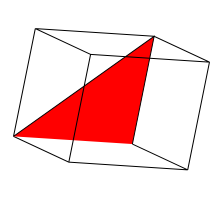
\includegraphics[scale=0.5]{figures/filling.png}
\caption{TODO. Can we find a simple triangulation or just simplification to use the fill() method on strictly convex sets?}

\end{figure}
\end{flushleft}


Convex sets contain the path between two points inside the set. That means, that the direct way from a to be is not crossing the borders of the set. This can be imagined with real borders of a set. A round set, or a rectangle have all points inside together with their path. A star for example, where you have two points at two of the tips is not convex, the direct path, the straight line would cross the border of the star, leave the star, and reenter the star. There is a formula, which gives the points on the path.

\begin{displaymath}
u = \lambda\vec{x} + (1-\lambda)\vec{y}, \lambda \in [0,1], x,y \in V \implies u \in V
\end{displaymath}

The factor lambda lies between 0 and 1. If $\lambda = 0.1$ then is $(1-\lambda) = 0.9$, if $\lambda = 0.2$ then is $(1-\lambda) = 0.8$ and so on. The result is lying on the straight line between $\vec{x}$ and $\vec{y}$. I have taken two vectors $\vec{x}, \vec{y} \in R^2$ and drawn them. The points lie on the line between the two points.

There is an inequality, which convex functions have to satisfy. And you may know it. It is the \emph{triangle inequality}

\begin{displaymath}
\|\lambda\vec{x} + (1-\lambda)\vec{y}\| \leq \lambda\|\vec{x}\| + (1-\lambda)\|\vec{y}\|
\end{displaymath}

or what expresses, that a function is convex.

\begin{displaymath}
f(\lambda\vec{x} + (1-\lambda)\vec{y}) \leq \lambda f(\vec{x}) + (1-\lambda)f(\vec{y})
\end{displaymath}

What is again the \emph{triangle inequality}.

Our image is very precise, because we designed a real coordinate system. What is happening to our new vector? 

\begin{displaymath}
\lambda\boldsymbol{A}\vec{x} + (1-\lambda)\boldsymbol{A}\vec{y} = \boldsymbol{A}(\lambda\vec{x} + (1-\lambda)\vec{y})
\end{displaymath}

By the rule of linearity.


\section{Definition of \mathbb{R}^{2\times3} (WORKING ON)}


\subsection{Defining the $(2\times3)\cdot(3\times1)$ as transitional operation to go from 3-D to 2-D}

The $\mathbb{R}^{2\times3}$ is a K-vectorspace. \\

It has scalar multiplication

\begin{displaymath}
(\lambda, \vec{x}) \mapsto \lambda\vec{x} 
\end{displaymath}

It has addition.

\begin{displaymath}
(\vec{u}, \vec{y}) \mapsto \vec{u} + \vec{x}
\end{displaymath}

You can add 2x3 matrices to 2x3, subtract 2x3 matrices from 2x3 matrices.
The addition of 2x3 matrices stays in the same subspaces.\\

The multiplication of the 2x3 matrices from the left or from the right changes to
the dimension of the resulting matrix.\\

The rule of thumb for matrix multiplication is $(m\times c)\cdot(c\times n)=(m\times n)$.\\

Here we multiply from the left, our 2x3 matrix is the right operand.\\

\begin{tabular}{-l-l-l-l-}
Left Operand & Right Operand & Resultant & Example\\
1x2 & 2x3 & 1x3&\\
2x2 & 2x3 & 2x3&\\
3x2 & 2x3 & 3x3&\\
4x2 & 2x3 & 4x3&\\
\end{tabular}\\

Here we multiply with the right, our matrix is the left operand.\\

\begin{tabular}{-l-l-l-}
Left Operand & Right Operand & Resultant\\
\textbf{2x3} & \textbf{3x1} & \textbf{2x1}& 3-D to 2-D mapping\\
2x3 & 3x2 & 2x2&\\
2x3 & 3x3 & 2x3&\\
2x3 & 3x4 & 2x4& \\
\end{tabular}\\

In my corollary about converting 4 dimensions onto the plane, there is this operation.

\begin{tabular}{-l-l-l-}
Left Operand & Right Operand & Resultant\\
\textbf{2x4} & \textbf{4x1} & \textbf{2x1}& 4-D to 2-D mapping\\
\end{tabular}\\

\newtheorem{PropositionOpt1}{Proposition. The $\mathbb{R}^{2\times3}$ operators have infinite combination possibilities $(m\times c)\cdot(c\times n)=(m\times n)$}
\begin{PropositionOpt1}
TODO
\end{PropositionOpt1}

Well, we are not alone in R2x3 with our coordinate transformation.\\

But. I want to come back to the main definition. \\

\newtheorem{PropositionOpt2}{Proposition. The $2\times3$ matrix operator is optimal for transforming 3-D into 2-D.}
\begin{PropositionOpt2}
With three coordinate axes as column vectors, arranged around the circle, deriving from the 2x3 standard basis with one linearly combined axis vector out of three, and a maximum of three linearly combined basis vectors by arrangement around the circle, the 2x3 matrix is an optimal operator for transforming 3x1 vectors (3-D vectors) into 2x1 vectors (2-D vectors).
\end{PropositionOpt2}

Remark. Got to prove it. Will find a good proof for.
\newtheorem{PropositionOpt4}{Proposition. Definition. Non-Standard Basis.}
\begin{PropositionOpt3}
A non-standard basis is something, which behaves like a basis, but is not a basis after the theorems. For example are the three axis vectors of the 2x3 matrix which transform and map three dimensions onto a 3-D coordinate system on the 2-D plane are a non-standard basis.
\end{PropositionOpt3}

\newtheorem{PropositionOpt4}{Proposition. Definition. 2x3 Non-Standard Basis.}
\begin{PropositionOpt4}
The first two intuitive non-standard basess for the 2x3 is the 90-degree $xy$ and 45 or 225 degree for $z$ combination, which has the values of the 2-D standard basis on two axes and a third one being exactly in the middle of both pointing into positive or negative direction with a value of $\pm\frac{1}\sqrt{2}$ or $\pm2^{-\frac12}$. The third one has an angle of 120 degrees between the axes and is arranged around the circle. The theorem is not finished.
\end{PropositionOpt3}

\newtheorem{PropositionOpt5}{Proposition. The $2\times3$ non-standard basis is the optimal 3-D coordinate system for the 2-D space.}
\begin{PropositionOpt5}
Modeled after a 3-D coordinate system on a piece of paper. Seen as a two dimensional image with two dimensional vectors. The 2x3 coordinate system is arranged as three vectors. One can arrange them around a circle using sine and cosine. The transformation brings a perfect linear mapping along the three vectors. The operation is moving the point from zero to the final point. The movements are decomposed into three horizontal and three vertical moves, where the coordinate is the scalar multiple of the axis vector each move.
\end{PropositionOpt5}

Ok. I have to formulate this out again.

\newtheorem{PropositionOpt6}{Proposition. The linear dependent vector can not be removed from the 2x3 basis.}
\begin{PropositionOpt6}
The 2x3 basis can not be reduced to the 2x1 basis with linear independent vectors, because the linear combination with the third vector is required to mix the coordinates for the image.
\end{PropositionOpt6}

Remark. TODO
Remark. (Lost the words i had in the bus)



\subsection{Orthogonality in the 2x3 matrix}


The 2x3 is mapping the 3-D input from $\begin{pmatrix}1&0&0\\0&1&0\\0&0&1\end{pmatrix}$ onto a 2-D plane. The 2-D plane itself follows the rules of orthogonal basis vectors. The standard basis for the R2 is $\begin{pmatrix}1&0\\0&1\end{pmatrix}$. Onto this basis the output of the 2x3 operators will be mapped.\\

Each of the three input coordinates, which regularly come from an orthogonal 3-D system, contributes a piece of movement to the two dimensions of the target space. One move is left or right, by cosine, and one is up or down by sine. On the plane the move is in a right angle against the other.\\

The 2x3 is combining 3 inputs into 2 outputs with $x\vec{e}_x + y\vec{e}_y + z\vec{e}_z$ by using the 2-D veectors as basis for the linear combinations.\\

The 2 outputs are then interpreted by the R2 standard basis as a linear combination of $\mu\begin{pmatrix}1\\0\end{pmatrix}+\nu\begin{pmatrix}0\\1\end{pmatrix}$.

\subsection{Orthogonal Projection from above}

To keep the orthogonality and orthogonal projection be two different words for two different things i add the paragraph directly here. An orthogonal projection is the shortest path from the point in 3-space to the 2-space plane. This is always the right angle directly onto the plane. This is the orthogonal projection, not to be intermingled with the orthogonal basis vectors being right angled. 

\subsubsection{Gram-Schmidt Orthogonalization}
\label{gram_schmidt_excercise}
We have not tried to orthogonalize the three axis vectors yet. In \cite{Strang1} one can read, how to do it.\\

From $\vec{e}_{n}$ we will calculate $\vec{q}_{n}$, the orthogonalized versions of the three axis vectors.\\

Our first vector is easy and just normalized. Using no r-value gives us the e-vector already normalized, but let us get through the three vectors.\\

\begin{displaymath}
\vec{q}_1 = \vec{e}_{x}/\|\vec{e}_{x}\|
\end{displaymath}

Now for the second vector. We remove the linear parts of the first from the second vector with $(q_{1}^{t}\vec{e}_{y})q_{1}$. (Maybe you recognize ($\vec{q}_{1}|\vec{e}_{y})\vec{q}_{1}$) from the orthogonal projection in Hilbert spaces.) In the second step the new vector is normalized by division by its magnitude

\begin{displaymath}
\begin{align}
\vec{b} &= \vec{e}_y - (\vec{q}_{1}^{T}\vec{e}_{y})\vec{q}_{1}\\
\vec{q}_{2} &= \frac{\vec{b}}{\|\vec{b}\|}
\end{align}
\end{displaymath}

And for the third vector we remove the linear parts of the other two vectors and normalize in the second step.

\begin{displaymath}
\begin{align}
\vec{c} &= \vec{e}_{z} - (\vec{q}_{1}^{T}\vec{e}_{z})\vec{q}_{1} - (\vec{q}_{2}^{T}\vec{e}_{z})\vec{q}_{2}\\
\vec{q}_{3} &= \frac{\vec{c}}{\|\vec{c}\|}
\end{align}
\end{displaymath}

Now we have three new vectors. In a $n\times n$ system, they will be linearly independent and form an orthogonal basis.\\


\textbf{Example. Righthand basis}\\

Consider this matrix:

\begin{displaymath}
    E^{\mathbb{R}^{2\times{3}}}_{y\perp z} = \begin{pmatrix}-2^{-\frac12}&0&1\\-2^{-\frac12}&1&0\end{pmatrix}
\end{displaymath}

This is the coordinate system with z-axis up, x pointing 225 degrees down south west, and y to the right.
On a piece of paper i applied Gram-Schmidt.

\begin{displaymath}
\begin{align}
\vec{e}_{x} &= \begin{pmatrix}-\sqrt{\frac12}\\-\sqrt{\frac12}\end{pmatrix}\\
\vec{e}_{y} &= \begin{pmatrix}1\\0\end{pmatrix}\\
\vec{e}_{z} &= \begin{pmatrix}0\\1\end{pmatrix}
\end{align}
\end{displaymath}

Remember. $-2^{-\frac12}$ is the same as $\cos 225$ and $\sin 225$. The length of this vector is already 1.

\begin{displaymath}
\begin{align}
\vec{e}_{x} &= \begin{pmatrix}-\sqrt{\frac12}\\-\sqrt{\frac12}\end{pmatrix}\\
\vec{q}_{1} &= \frac{\vec{e}_{x}}{\|\vec{e}_{x}\|} = \vec{e}_{x}
\end{align}
\end{displaymath}

Now for the second vector\\

\begin{displaymath}
\begin{align}
\vec{e}_{y} &= \begin{pmatrix}1\\0\end{pmatrix}\\
	\vec{b} &= \begin{pmatrix}1\\0\end{pmatrix} - 
	(\begin{pmatrix}-\sqrt{\frac12}&-\sqrt{\frac12}\end{pmatrix}
	\begin{pmatrix}1\\0\end{pmatrix})
	\begin{pmatrix}-\sqrt{\frac12}\\-\sqrt{\frac12} \end{pmatrix}\\
	&= \begin{pmatrix}\frac12\\-\sqrt{\frac12}\end{pmatrix}\\
	\vec{q}_{2} &= \frac{\vec{b}}{\|\vec{b}\|}
			= \begin{pmatrix}\frac{\frac12}{\frac14 + \frac12}\\\frac{-\sqrt{\frac12}}{\frac34}\end{pmatrix} 
			= \begin{pmatrix}\frac23\\-\frac43 \sqrt{\frac12}\end{pmatrix}\\    
\end{align}
\end{displaymath}

And for the third vector.\\

\begin{displaymath}
\begin{align}
\vec{e}_{y} &= \begin{pmatrix}0\\1\end{pmatrix}\\
\vec{c} &= \vec{e}_{z} - (\vec{q}_{1}^{T}\vec{e}_{z})\vec{q}_{1} - (\vec{q}_{2}^{T}\vec{e}_{z})\vec{q}_{2}\\
			&= \begin{pmatrix}0\\1\end{pmatrix} - \begin{pmatrix}\frac12\\\frac12\end{pmatrix}-(-\frac43\sqrt{\frac12})\begin{pmatrix}\frac46\\-\frac43\sqrt{\frac12}\end{pmatrix}\\
\vec{q}_{3} = \frac{\vec{c}}{\|c\|}
			&= \begin{pmatrix}-\frac{25}{18}\\-\frac{7}{18}\end{pmatrix}
\end{align}
\end{displaymath}

Gram Schmidt gave us these vectors.
\begin{displaymath}
\begin{align}
\vec{q}_{1} &=  \begin{pmatrix}-\sqrt{\frac12}\\-\sqrt{\frac12}\end{pmatrix}\\
\vec{q}_{2} &= \begin{pmatrix}\frac46\\-\sqrt{\frac{8}{9}}\end{pmatrix}\\
\vec{q}_{3} &= \begin{pmatrix}-\frac{25}{18}\\-\frac{7}{18}\end{pmatrix}
\end{align}
\end{displaymath}



\subsubsection{Screenshot of after Gram-Schmidt}

I decided to take the 45 degree perspective projection of a cube. I patched the code and the implement.js\\

\begin{figure}[ht]
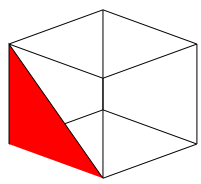
\includegraphics[scale=0.5]{figures/b4ortho.png}
\caption{Before Gram Schmidt. This is the 45 degree lefthand basis.}
\end{figure}

I do not know how big the error of the used source code is. My second screenshot, typing handwritten results in, is not there yet.\\

\begin{figure}[ht]
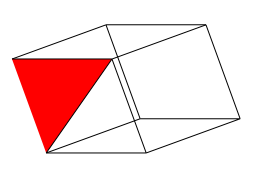
\includegraphics[scale=0.5]{figures/afterortho.png}
\caption{After Gram Schmidt. It seems very fine for this experiment. The angles have changed. But it is very fine when rotated. }
\end{figure}

I do not clean up the code today. This is the little patch, with which i went over my axis vectors. The perspective changes a little, and it is still wonderful. \\


\textbf{Example} JavaScript example code without any error correction. So this is NOT exact. But gives a wonderful insight.

\begin{lstlisting}
function gs_ortho(ex,ey,ez) {
    var norm_ex = norm(ex,2);
    var q1 = [ ex[0]/norm_ex, ex[1]/norm_ex ];
    var tmp = (q1[0] * ey[0] + q1[1] * ey[1]); // q1^t*ey
    var b = [ ey[0] - (tmp*q1[0]),
	      ey[1] - (tmp*q1[1]) ];
    var norm_b = norm(b,2);
    var q2 = [b[0]/norm_b, b[1]/norm_b];
    var tmp1 = (q1[0] * ez[0] + q1[1] * ez[1]);
    var tmp2 = (q2[0] * ez[0] + q2[1] * ez[1]);
    var c = [
	ez[0] - (tmp1*q1[0]) - (tmp2*q2[0]),
	ez[1] - (tmp1*q1[1]) - (tmp2*q2[1])
    ];
    var norm_c = norm(c,2);
    var q3 = [
	c[0]/norm_c, c[1]/norm_c
    ];
    return [q1,q2,q3];
}
\end{lstlisting}



\subsection{Intuitive standard basis for multiplying with 3x1}
\label{intuitive_standard_basis}
First off, the optimal non-standard basis is still arranged around the circle, like at the beginning explained.\\

Remark. When talking of a basis here, we talk with a background of knowing that this is not a linear independent vector space basis, but the only right coordinate system, which is used like a basis, which induces a linear map or a linear combination of three vectors on two dimensions.\\

When deducing from the format of the R2x3 basis, the first suggestions are to use zeros and ones for the basis. The very intuitive first guess using our already defined lefthanded and righthanded systems are these:\\

\begin{displaymath}
    E^{\mathbb{R}^{2\times{3}}}_{lefthand} = \begin{pmatrix}1&0&1\\0&1&1\end{pmatrix} \mbox{ and }
    E^{\mathbb{R}^{2\times{3}}}_{righthand} = \begin{pmatrix}-1&1&0\\-1&0&1\end{pmatrix}
\end{displaymath}

The thing is, the vectors are not normalized in that case (see \ref{why_normalize} for an example, why normalization is sometimes required). We have to do so. If we have two ones, the squared sum is two. The square root out of two is the square root of two. $2^{-\frac12}$ is the normalized length of a vector containing two ones.\\

What else can you see? The standard basis of $\mathbb{R}^{2}$ embedded in the $\mathbb{R}^{2\times3}$ matrix.\\

\begin{displaymath}
    E^{\mathbb{R}^{2\times{3}}}_{x\perp y} = \begin{pmatrix}1&0&2^{-\frac12}\\0&1&2^{-\frac12}\end{pmatrix} \mbox{ and }
    E^{\mathbb{R}^{2\times{3}}}_{y\perp z} = \begin{pmatrix}2^{-\frac12}&0&1\\2^{-\frac12}&1&0\end{pmatrix} \mbox{ and }
    E^{\mathbb{R}^{2\times{3}}}_{x\perp z} = \begin{pmatrix}1&2^{-\frac12}&0\\0&2^{-\frac12}&1\end{pmatrix} 
\end{displaymath}

Can you spot, what i did? I embedded the third axis in some orthogonal 2-D system. Here the axes point into the same positive direction, this is a lefthand system. We look from the back into the z direction.


\begin{displaymath}
    E^{\mathbb{R}^{2\times{3}}}_{x\perp y} = \begin{pmatrix}1&0&-2^{-\frac12}\\0&1&-2^{-\frac12}\end{pmatrix} \mbox{ and }
    E^{\mathbb{R}^{2\times{3}}}_{y\perp z} = \begin{pmatrix}-2^{-\frac12}&0&1\\-2^{-\frac12}&1&0\end{pmatrix} \mbox{ and }
    E^{\mathbb{R}^{2\times{3}}}_{x\perp z} = \begin{pmatrix}1&-2^{-\frac12}&0\\0&-2^{-\frac12}&1\end{pmatrix} 
\end{displaymath}

Here the additional axis shows in the other direction. This is a righthand system. We look from the front against the x direction.
Which is pointing towards us, left down. The y axis is pointing to the right and the z axis to the up.\\

\textbf{With the dot product we test for linear independence}\\

To test the linear independence of two vectors, their dot product must equal zero.\\
That means, the two vectors are perpendicular $\perp$ to each other. They meet in a right angle. As you already know, 
in our 2x3 system it is not possible to give three independent vectors. You can have one to three linear combinations.\\


In our coordinate system, we have to test for $\vec{e}_{x}\cdot\vec{e}_{y}$, $\vec{e}_{x}\cdot\vec{e}_{z}$ and $\vec{e}_{y}\cdot\vec{e}_{z}$.

We test the "embedded" coordinate system with the $\mathbb{R}^{2}$ standard basis and the one linear dependent vector. We 
get another stoking result containing parts of our axis vectors, of course.\\

For the righthand system:\\

\begin{displaymath}
\begin{align}
\vec{e}_{x}\cdot\vec{e}_{y} &= -2^{-\frac12}*1 + -2^{-\frac12}*0 = -2^{-\frac12} = \cos225^{\circ}\\
\vec{e}_{x}\cdot\vec{e}_{z} &= -2^{-\frac12}*0 + -2^{-\frac12}*1 = -2^{-\frac12} = \sin225^{\circ}\\
\vec{e}_{y}\cdot\vec{e}_{z} &= 1*0+0*1 = 0\\
\end{align}
\end{displaymath}

Only the third pair is orthogonal. Two pairs are not. And that in the best case config for orthogonality.\\

For the lefthand system:\\

\begin{displaymath}
\begin{align}
\vec{e}_{x}\cdot\vec{e}_{y} &= 1*0+0*1 = 0\\
\vec{e}_{x}\cdot\vec{e}_{z} &= 1*2^{-\frac12} + 0*2^{-\frac12} = 2^{-\frac12} = \cos45^{\circ}\\
\vec{e}_{y}\cdot\vec{e}_{z} &= 0*2^{-\frac12} + 1*2^{-\frac12} = 2^{-\frac12} = \sin45^{\circ}\\
\end{align}
\end{displaymath}

Only the first pair is orthogonal. The other result in the sin and cosine parts, one for one of the two pairs, due to the mix with the orthogonal pair.\\

\subsection{Deconstructing the 2x3 basis} 

\fbox{The whole section about R2x3 is to be continued very soon}

Remark. This example concerning the book \cite{Strang1} seems to be about R6 and not to match my interpretation.\\

In the Appendix of \cite{Strang1}, there is a basis of a 2x3 matrix printed, together with a few arguments. The professor constructed a 2x3 standard basis by multiplying the 2-D standard basis vectors with the 3-D standard vectors. A 2x3 basis is a set of six matrices being constructed out of five basis vectors according to the books. \\

\begin{displaymath}
\begin{center}
e_{1}^{\mathbb{R}^{2}} = \begin{pmatrix}1\\0\end{pmatrix}
e_{2}^{\mathbb{R}^{2}} = \begin{pmatrix}0\\1\end{pmatrix}\\

e_{1}^{\mathbb{R}^{3}} = \begin{pmatrix}1\\0\\0\end{pmatrix}
e_{2}^{\mathbb{R}^{3}} = \begin{pmatrix}0\\1\\0\end{pmatrix}
e_{2}^{\mathbb{R}^{3}} = \begin{pmatrix}0\\0\\1\end{pmatrix}

\end{center}
\end{displaymath}

Multiplying $e_{i}^{\mathbb{R}^{2}}$ with $(e_{j}^{\mathbb{R}^{3}})^{T}$ yields six independent matrices, which, when added, form the standard basis.

\begin{displaymath}
E^{\mathbb{R}^{2\times{3}}} =
\begin{pmatrix}1&0&0\\0&0&0\end{pmatrix}+
\begin{pmatrix}0&1&0\\0&0&0\end{pmatrix}+
\begin{pmatrix}0&0&1\\0&0&0\end{pmatrix}+
\begin{pmatrix}0&0&0\\1&0&0\end{pmatrix}+
\begin{pmatrix}0&0&0\\0&1&0\end{pmatrix}+
\begin{pmatrix}0&0&0\\0&0&1\end{pmatrix}

\end{displaymath}

Replacing the ones with variables, we get the following.

\begin{displaymath}
\begin{center}
e_{1}^{\mathbb{R}^{2}} = \begin{pmatrix}u\\0\end{pmatrix}
e_{2}^{\mathbb{R}^{2}} = \begin{pmatrix}0\\v\end{pmatrix}\\
e_{1}^{\mathbb{R}^{3}} = \begin{pmatrix}a\\0\\0\end{pmatrix}
e_{2}^{\mathbb{R}^{3}} = \begin{pmatrix}0\\b\\0\end{pmatrix}
e_{2}^{\mathbb{R}^{3}} = \begin{pmatrix}0\\0\\c\end{pmatrix}\\
E^{\mathbb{R}^{2\times{3}}} =
\begin{pmatrix}ua&0&0\\0&0&0\end{pmatrix}+
\begin{pmatrix}0&ub&0\\0&0&0\end{pmatrix}+
\begin{pmatrix}0&0&uc\\0&0&0\end{pmatrix}+
\begin{pmatrix}0&0&0\\va&0&0\end{pmatrix}+
\begin{pmatrix}0&0&0\\0&vb&0\end{pmatrix}+
\begin{pmatrix}0&0&0\\0&0&vc\end{pmatrix}
\end{center}
\end{displaymath}
Here we can subtitute
\begin{displaymath}
ua=r_x\cos\varphi_x,
va=r_x\sin\varphi_x,
ub=r_y\cos\varphi_y,
vb=r_y\sin\varphi_y,
uc=r_z\cos\varphi_z,
vc=r_z\sin\varphi_z,
\end{displaymath}
It should result in
\begin{displaymath}
\begin{center}
\begin{pmatrix}r_x\cos\varphi_x&0&0\\0&0&0\end{pmatrix}+
\begin{pmatrix}0&r_y\cos\varphi_y&0\\0&0&0\end{pmatrix}+
\begin{pmatrix}0&0&r_z\cos\varphi_z\\0&0&0\end{pmatrix}+\\
\begin{pmatrix}0&0&0\\r_x\sin\varphi_x&0&0\end{pmatrix}+
\begin{pmatrix}0&0&0\\0&r_y\sin\varphi_y&0\end{pmatrix}+
\begin{pmatrix}0&0&0\\0&0&r_z\sin\varphi_z\end{pmatrix}\\
   = \begin{pmatrix}
    r_x\cos\varphi_x & r_y\cos\varphi_y & r_z\cos\varphi_z \\
    r_x\sin\varphi_x & r_y\sin\varphi_y & r_z\sin\varphi_z \\
    \end{pmatrix}
\end{center}
\end{displaymath}

That does not solve the problem. It is my first guess from the day, where i spotted the example.\\

\section{Proving more rules of the main formula TODO}

The 'hardest' part is the SVD of the rectangular matrix. I suspect the axis vectors to be the results, but can not prove until i calculate. And i suspect, that every angle changes the singular values, like it changes the eigenvalues of AAt and AtA.\\

The SVD is not that hard. Hard is the handwritten version without numbers with the trigonometric functions, because the terms become very long, and maybe substitution is neccessary to write. I will fix it soon.\\



\subsubsection{Singular Value Decomposition}

TODO\\

This a mxm orthogonal times nxm diagonal times nxn orthogonal. To get the orthogonal we have to take the eigenvectors from the products with the transpose. TODO.\\

\begin{displaymath}
    \boldsymbol{A} = \boldsymbol{U}\boldsymbol{\Sigma}\boldsymbol{V}^{T}
\end{displaymath}

Remark. A rectangular matrix has no eigenvalue equation (like no direct inverse). But there is a singular value decomposition, which can tell some proper things about the matrix. For that, the eigenvalues are taken from the products with the transpose. And then the decomposition continues.\\

The $A^{T}A$ and $AA^{T}$ are needed for the SVD. First we extract the eigenvalues and eigenvectors of the symmetric square matrices.
$((A^{T}A)-\lambda{I})x=0$ and $((AA^{T})-\lambda{I})x=0$ need to be solved.\\

\subsection{Eigenvalues and -vectors of the 2x2 $AA^{T}$ to reach U}
\label{eig_2x3}

\textbf{Example}
Multiplying the intutitive standard basis from \ref{intuitive_standard_basis} gives

\begin{displaymath}
\boldsymbol{A}\boldsymbol{A}^{T} = \begin{pmatrix}\frac32&\frac12\\\frac12&\frac32\end{pmatrix}
\end{displaymath}

Solving $det(A-\lambda I)=0$ gives us the characteristic polynomial and after foiling and simplification

\begin{displaymath}
\begin{align}
(\frac32-\lambda)^{2}-\frac14\\
=& \lambda^{2}-3\lambda+2\\
=& (\lambda-1)(\lambda-2)
\end{align}
\end{displaymath}

This gives use the poles and the eigenvalues
\begin{displaymath}
\begin{align}
\lambda_{1} &= 1\\
\lambda_{2} &= 2
\end{align}
\end{displaymath}

Subtracting the Eigenvalues from the matrix and solving for the eigenvectors gives me (quick notes from underways on the backside of \cite{Kuehn1})

\begin{displaymath}
\begin{align}
\boldsymbol{A}\boldsymbol{A}^{T}-\lambda_{1}I &= \begin{pmatrix}{\frac12&\frac12\\\frac12&\frac12}\end{pmatrix}\\
\xi_{1} &= \begin{pmatrix}1\\1\end{pmatrix}\\
\boldsymbol{A}\boldsymbol{A}^{T}-\lambda_{2}I &= \begin{pmatrix}{-\frac12&\frac12\\\frac12&-\frac12}\end{pmatrix}\\
\xi_{2} &= \begin{pmatrix}1\\-1\end{pmatrix}\\
\end{align}
\end{displaymath}

This brings me to U of our SVD

\begin{displaymath}
\boldsymbol{U} = \begin{pmatrix}1&1\\1&-1\end{pmatrix}
\end{displaymath}

\subsection{Eigenvalues and -vectors of the 3x3 $A^{T}A$}

\textbf{Possibly wrong}. The determinant could be zero, the polynomial just $(1-\lambda)^{2}$ and the eigenvalues $0,1,1$. The following is from my first notes. The second determinant gave zero, and thinking about gave me the previous results. But now the notes, for the next few days, they are fun in this document.\\

\textbf{Example}\\

After solving for the 2x2 i started solving for the 3x3 with a pen.

\begin{displaymath}
\boldsymbol{A}^{T}\boldsymbol{A} = \begin{pmatrix}1&-2^{-\frac12}&-2^{-\frac12}\\-2^{-\frac12}&1&0\\-2^{-\frac12}&0&1\end{pmatrix}
\end{displaymath}

Underways i subtracted lambda and solved for the determinant using the crossproduct and determinat formula for handwritten determinants of 3x3 matrices.\\

\begin{displaymath}
\boldsymbol{A}^{T}\boldsymbol{A} = \begin{pmatrix}1-\lambda&-2^{-\frac12}&-2^{-\frac12}\\-2^{-\frac12}&1-\lambda&0\\-2^{-\frac12}&0&1-\lambda\end{pmatrix}
\end{displaymath}
By the way. My notes say, the determinant is
\begin{displaymath}
|\boldsymbol{A}^{T}\boldsymbol{A}| = \frac32
\end{displaymath}

Mean, i wanted to fetch the notes, but can not find it. I remember from writing underways, that i only found one pole from
\begin{displaymath}
(1-\lambda)^{2}-(1-\lambda)
\end{displaymath}
which was the result of the determinant minus lambda or the characteristic polynomial. Yes, i only solved the first trivial pole
\begin{displaymath}
\lambda_{2}=1
\end{displaymath}

Solving then for the eigenvector, i got this possible solution for $(\boldsymbol{A}^{T}\boldsymbol{A}-\lambda I)\vec{x}=0$. The first one is 0 because subtracting lamda from the diagonal gave me zero on the whole diagonal.

\begin{displaymath}bb
\boldsymbol{A}^{T}\boldsymbol{A}-\lambda{I} = \begin{pmatrix}0&-2^{-\frac12}&-2^{-\frac12}\\-2^{-\frac12}&0&0\\-2^{-\frac12}&0&0\end{pmatrix}
\end{displaymath}
Solving for the non-zero vector, which results in the zero vector, gives me for $\lambda_{1}$
\begin{displaymath}
\vec{\xi}_{2} = \begin{pmatrix}0\\1\\-1\end{pmatrix}
\end{displaymath}

If this is correct, this is our first eigenvector. If not, i will verify it next time\\

Somewhere here our journey with the bus and subways was over and i have got to come back to the topic soon.\\

On the next morning i looked at the polynomial and got at once the second eigenvalue. It is the zero.
\begin{displaymath}
(1-0)^{2}-(1-0) = 1-1 = 0
\end{displaymath}
So our second eigenvalue, which in order is now the first eigenvalue, is $\lambda_1 = 0$. Installed in our Eigenvector Equation it is just the matrix we started with, because subtracting zero from the diagonal does not change anything.
\begin{displaymath}
(\boldsymbol{A}^{T}\boldsymbol{A}-0I) = \begin{pmatrix}1&-2^{-\frac12}&-2^{-\frac12}\\-2^{-\frac12}&1&0\\-2^{-\frac12}&0&1\end{pmatrix}
\end{displaymath}
Now solve for $(\boldsymbol{A}^{T}\boldsymbol{A}-0I)\vec{x}=0$.
\begin{displaymath}
\end{displaymath}

Oh, and i forgot. A 3x3 polynomial should have three roots. Simplifying $(1-\lambda)^{2}(1-\lambda)$ gives $\lambda^{2}-3\lambda = 0$

\begin{displaymath}
\begin{center}
\lambda^{2}-3\lambda = 0\\
\lambda^{2} = 3\lambda\\
\lambda = 3
\end{center}
\end{displaymath}

So we have all three roots (eigenvalues) together. I have to solve for the remaining two eigenvectors. The 0 value gave a system i still have to solve (underways i started).\\

\begin{displaymath}
\lambda_{1} = 0\qquad\lambda_{2}=1\qquad\lambda_{3}=3
\end{displaymath}

Remark. Nice to get some excercise for this topic.

Remark II. The 3x3 can be mistaken. My last test for the determinant of AtA gave 0, i have to verify this again.

If we have $\boldsymbol{U}$ and $\boldsymbol{V}^{T}$ we can get $\Sigma$ by using $\boldsymbol{A}$
\begin{displaymath}
 \boldsymbol{U}^{T}\boldsymbol{A}\boldsymbol{V} = \boldsymbol{\Sigma}
\end{displaymath}


\subsubsection{The pseudo-inverse $\boldsymbol{A}^{+}$}

For a m by n matrix with m < n it is $A^T(AA^{T})^{-1}$\\

This is easily calculated. For the coordinate system with the 45 degree z axis beetween the default x-y axes on the plane the $2 \times 2$ matrix for $AA^T$ is simply

\begin{displaymath}
	AA^T = \begin{pmatrix}\frac32 & \frac12\\ \frac12 & \frac32
	\end{pmatrix}
\end{displaymath}

The determinant is $(\frac32)^2 - (\frac12)^2 = 2$. And the inverse is 

\begin{displaymath}
\begin{align}
	(AA^T)^{-1} &= \frac12\begin{pmatrix}\frac32 & -\frac12 \\ -\frac12 & \frac32 \end{pmatrix}\\
	&= \begin{pmatrix}\frac34 & -\frac14 \\ -\frac14 & \frac34 \end{pmatrix}
\end{align}
\end{displaymath}

Now we multiply the $3 \times 2$ matrix $A^T$ with the inverse of the $2 \times 2$ matrix and obtain the Moore-Penrose Inverse, also known as the pseudo inverse of A.

\begin{displaymath}
\begin{align}
	A^{\dagger} = A^T (AA^T)^{-1} &= \begin{pmatrix}
	1&0\\
	0&1\\
	2^{-\frac12}&
	2^{-\frac12}
	\end{pmatrix} \begin{pmatrix}\frac34 & -\frac14 \\ -\frac14 & \frac34 \end{pmatrix}
\end{align}
\end{displaymath}

I have decided to write, when writing manually, the coefficients downwards, instead of messing up the piece of paper, by filling the sums into the matrix.

\begin{displaymath}
\begin{align}
	a_11 &= 1* \frac34 + 0*-\frac14 = \frac34\\
	a_12 &= 1* -\frac14 + 0*\frac34 = -\frac14\\
	a_21 &= 0* \frac34 + 1*-\frac14 = -\frac14\\
	a_22 &= 0* -\frac14 + 1*\frac34 = \frac34\\	
	a_31 &=2^{-\frac12} * \frac34 + 2^{-\frac12}*-\frac14 = 2^{-\frac12}(\frac12) = 8^{-\frac12}\\
	a_32 &=2^{-\frac12} * -\frac14 + 2^{-\frac12}*\frac34 = 2^{-\frac12}(\frac12) = 8^{-\frac12}\\
\end{align}
\end{displaymath}

I wrote it down to leave it as a hint, how to keep the paper cleaner, if you´d like to try it on your own.

The resulting pseudo inverse is this

\begin{displaymath}
A^{\dagger} = \begin{pmatrix}
	\frac34 & -\frac14 \\
	-\frac14 & \frac34 \\
	8^{-\frac12} & 8^{-\frac12}
\end{pmatrix}
\end{displaymath}







For a m by n matrix with m > n it is $(A^{T}A)^{-1}A^T$\\
TODO\\

\section{Computer Error Estimation}

The error $e$ is the absolute value of the exact result $x$ and the computed result $\hat{x}$.

\begin{displaymath}
e = |x - \hat{x}|
\end{displaymath}

In more than one dimension it is the same. The computed result is subtracted from the exact result.

\begin{displaymath}
\vec{e} = \|\vec{x} - \hat{\vec{x}}\|
\end{displaymath}


TODO

Remark. The roundoff error of the floating point and the condition of a matrix is basic knowledge for every computer class.

\section{An alternative graphics algorithm}

\textbf{Remark} This section is new on July 10.

It is obvious, that we want to draw some graphics on our 2-D Canvas. This works on any graphics surface, where you can connect 2-D points with methods, or draw then directly, by changing pixels.

Remark. Missing. The fill algorithm (the stuff is pretty long) and our view frustum (). Plus the remark, we do not try to replace computer graphics. But for small visualizations it is a quick tool, for handwritten code.\\

\subsection{Origin}  

Setting the origin is an easy task. Assuming, the regular origin is at (0,0,0) and (0,0), we just need to add the shift to the coordinate. You can shift the 3-D Origin or the 2-D Origin.  It is just a translation.\\

\begin{lstlisting}
x = Ox + x;
y = Oy + y;
z = Oz + z;
\end{lstlisting}

This has to be applied to every point.

\subsection{Translation}

You simply add the translation vector to each point.\\

Remark. This is the same like shifting the origin, but translation has a meaning, that it is then done, maybe a few times, with animation, to move from a to b.

\begin{lstlisting}
x = Tx + x;
y = Ty + y;
z = Tz + z;
\end{lstlisting}

Remark. A affine combination is written $x = a + Ax$. So to say, the same for the origin.

\subsection{Scaling}

To scale the object you just have to multiply with the constant. 

\begin{lstlisting}
x = Sx * x;
y = Sy * y;
z = Sz * z;
\end{lstlisting}


\subsection{Skewing}

Skewing or shearing is not difficult. I took a skewing matrix and forgot about the empty fields.

\begin{lstlisting}
u = x, v = y, w = z;
x =      u + k_xy*v + k_xz*w;
y = k_yx*u + v      + k_yz*w;
z = k_zx*u + k_zy*v + w;
\end{lstlisting}

\subsection{Local 3x3 basis for change of units and per object rotation}

If you wish to introduce different units for different directions, you have to apply a local basis, if the picture is moving angular. Applying the local 3x3
basis to an object makes sure, it will be rotatable, but without side effects. If you would change the units of r on the projection, then the rotation will give unrealistic results, since suddenly the object stretches to an unexpected size, when entering the zone. \\

The matrix applied locally is a 3x3 matrix $\begin{pmatrix} xBX & yBX & zBX\\ xBY & yBY & zBY\\ xBZ & yBZ & zBZ\end{pmatrix}$.
For example is $\begin{pmatrix} 1 & 0 & 0\\ 0 & 1 & 0\\ 0 & 0 & 1\end{pmatrix}$ is the original and orthonormal (orthogonal and unit length) standard basis for the $\mathbb{R}^{3}$ and the result is the same as if you do not apply any basis to the object, as the assumed default coordinate system in $\mathbb{R}^{3}$ is orthonormal.\\

\begin{lstlisting}
u = x, v = y, w = z;
x = u*xBX + v*yBX + w*zBX;
y = u*xBY + v*yBY + w*zBY;
z = u*xBZ + v*yBZ + w*zBZ;
\end{lstlisting}

This of course transforms the object by the directions and the length of the three three dimensional basis vectors.

\subsubsection{Creating a 3x3 basis with cross products}
\begin{lstlisting}
function cross(a,b) {
    // does not multiply with the ijk components, diy
    return [a[1]*b[2]-a[2]*b[1],-a[0]*b[2]+a[2]*b[0],a[0]*b[1]-a[1]*b[0]];
}
\end{lstlisting}

// if you look and remember \ref{crossproducts} you see the third determinant only giving (1-0)k
\begin{lstlisting}
var u = [1,0,0];
var v = [0,1,0]; 
var w = cross(u,v);
// w = [0,0,1]
\end{lstlisting}
// if you look and remember \ref{crossproducts} you see the third determinant only giving (-1-0)k
\begin{lstlisting}
var u = [-1,0,0];
var v = [0,1,0];
var w = cross(u,v);
// w = [0,0,-1]
\end{lstlisting}

\subsection{Rotation}

Rotating the object can be done in three dimensional space by applying the regular rotation matrices. 

\begin{lstlisting}
// once
    var rotxcos = Math.cos(xAngleRad), rotxsin = Math.sin(xAngleRad);
    var rotycos = Math.cos(yAngleRad), rotysin = Math.sin(yAngleRad);
    var rotzcos = Math.cos(zAngleRad), rotzsin = Math.sin(zAngleRad);
// for each point
    u = x, v = y, w = z;
    y = v * rotxcos - w * rotxsin
    z = v * rotxsin + w * rotxcos
    u = x, v = y, w = z;
    x =  u * rotycos + w * rotysin;
    z = -u * rotysin + w * rotycos;
    u = x, v = y, w = z;
    x = u * rotzcos - v * rotzsin;
    y = u * rotzsin + v * rotzcos;
\end{lstlisting}

\subsection{Frustum and Perspective}

Apply the perspective to the 3x3 set of points before projecting.

\begin{lstlisting}
TODO
\end{lstlisting}


\subsection{Dot product}

The dot product or inner product or scalar product is the sum of the component products and one of the most important basic formulas in space.\\

\begin{lstlisting}
function dot(a,b) {
    var sum = 0;
    for (var i = 0, j = a.length; i < j; i++) sum += a[i]*b[i];
    return sum;
}
\end{lstlisting}

\subsection{Norm}

The euclidean norm is the length of the vector. It´s the square root pulled out of the sum of all components squared.\\

\begin{lstlisting}
function norm(a) {
    var sum = 0;
    for (var i = 0, j = a.length; i < j; i++) sum += a[i]*a[i];
    return Math.sqrt(sum);
}
\end{lstlisting}\\

A p-Norm version, the second argument is the exponent p and p-th root.\\

\begin{lstlisting}
function norm(a,p) {
    var sum = 0;
    if (p===undefined) p = 2;
    if (p===Infinity) {
        var max = 0;
        for (var i = 0, j = a.length; i < j; i++) {
            max = Math.max(Math.abs(a[i]), max);
        }
        return max;
    }
    for (var i = 0, j = a.length; i < j; i++) sum += Math.pow(Math.abs(a[i]),p);
    for (i = 2; i <= p; i++) sum = Math.sqrt(sum);
    return sum;
}
\end{lstlisting}

\subsection {Metric}

The distance function gives us the distance between two points, that is the length of the vector from tip to tip.

\begin{lstlisting}
function d(a,b) {
    var sum = 0;
    for (var i = 0, j = a.length; i < j; i++) sum += Math.pow(a[i]-b[i],2);
    return Math.sqrt(sum);
}
\end{lstlisting}


\subsection{Code Example}

Here is an implementation of these function together with the EcmaScript 6 snippet in modern EcmaScript 5.\\

These functions are not optimized for speed. Each of the -all functions take the whole set of points, so 
the complexity rises to n times iterating over the point sets. To create faster code, you got to inline your
code and do everything in the right order in one loop. Anyways, that is not difficult and intuitive to programmers.\\


\begin{lstlisting}
(function (exports) {

function rad(deg) { 
    return Math.PI/180*deg; 
}

var r_x = 1, r_y = 1, r_z = 1;

var phi_x = rad(210), phi_y = rad(330), phi_z = rad(90);

var xAxisCos = r_x * Math.cos(phi_x),
    yAxisCos = r_y * Math.cos(phi_y),
    zAxisCos = r_z * Math.cos(phi_z),
    xAxisSin = r_x * Math.sin(phi_x),
    yAxisSin = r_y * Math.sin(phi_y),
    zAxisSin = r_z * Math.sin(phi_z);

function transform2d(vec3) {
    return [
    vec3[0]*xAxisCos + vec3[1]*yAxisCos + vec3[2]*zAxisCos,
    vec3[0]*xAxisSin + vec3[1]*yAxisSin + vec3[2]*zAxisSin
    ];
}

function transform2dAll(avec3) {
    return avec3.map(transform2d);
}

function settrans(op) {
    if (op.phi_n) {
    phi_x = op.phi_n[0];
    phi_y = op.phi_n[1];
    phi_z = op.phi_n[2];
    }
    if (op.r_n) {
    r_x = op.r_n[0];
    r_y = op.r_n}[1];
    r_z = op.r_n[2];
    }
    xAxisCos = r_x * Math.cos(phi_x);
    yAxisCos = r_y * Math.cos(phi_y);
    zAxisCos = r_z * Math.cos(phi_z);
    xAxisSin = r_x * Math.sin(phi_x);
    yAxisSin = r_y * Math.sin(phi_y);
    zAxisSin = r_z * Math.sin(phi_z);
}

function gettrans() { 
    return { 
    phi_n: [phi_x, phi_y, phi_z], 
    r_n: [r_x, r_y, r_z] 
    }; 
}

function draw2dAll(ctx, points2, scale) {
    ctx.save();
    scale = scale || 1;
    var x = scale * points2[0][0], y = scale * points2[0][1];
    ctx.moveTo(x,-y);
    ctx.beginPath();
    for (var i = 0, j = points2.length; i < j; i++) {
    x = scale * points2[i][0], y = scale * points2[i][1];
    ctx.lineTo(x,-y);
    ctx.moveTo(x,-y);
    }
    ctx.closePath();
    ctx.stroke();
    ctx.restore();
}

function rotate3dAll(xAngleRad,yAngleRad,zAngleRad, points3) {
    var rotxcos = Math.cos(xAngleRad), rotxsin = Math.sin(xAngleRad);
    var rotycos = Math.cos(yAngleRad), rotysin = Math.sin(yAngleRad);
    var rotzcos = Math.cos(zAngleRad), rotzsin = Math.sin(zAngleRad);
    var p, x, y, z, u, v, w;
    for (var i = 0, j = points3.length; i < j; i++) {
        p = points3[i], x = p[0], y = p[1], z = p[2];
        u = x, v = y, w = z;
        y = v * rotxcos - w * rotxsin
        z = v * rotxsin + w * rotxcos
        u = x, v = y, w = z;
        x = u * rotycos + w * rotysin;
        z = -u * rotysin + w * rotycos;
        u = x, v = y, w = z;
        x = u * rotzcos - v * rotzsin;
        y = u * rotzsin + v * rotzcos;
        p[0]=x;
        p[1]=y;
        p[2]=z;
    }
}
    
function rotate2dAll(zAngle, points2) {
    var rotzcos = Math.cos(zAngleRad), rotzsin = Math.sin(zAngleRad);
    var p, x, y, u, v;
    for (var i = 0, j = points2.length; i < j; i++) {
        p = points2[i], x = p[0], y = p[1];
        u = x, v = y;
        x = u * rotzcos - v * rotzsin;
        y = u * rotzsin + v * rotzcos;
        p[0]=x;
        p[1]=y;
    }
}

function translate3dAll(transvec, points3) {
    var p, x, y, z;
    var Tx = transvec[0],
    Ty = transvec[1],
    Tz = transvec[2];
    for (var i = 0, j = points3.length; i < j; i++) {
        p = points3[i];
        p[0]+=Tx;
        p[1]+=Ty;
        p[2]+=Tz;
    }
}

function translate2dAll(transvec, points2) {
    var p;
    var Tx = transvec[0],
    Ty = transvec[1];
    for (var i = 0, j = points2.length; i < j; i++) {
        p = points2[i];
        p[0]+=Tx;
        p[1]+=Ty;
    }
}

function scale3dAll(scaleX, scaleY, scaleZ, points3) {
    var p;
    for (var i = 0, j = points3.length; i < j; i++) {
        p = points3[i];
        p[0]*=scaleX;
        p[1]*=scaleY;
        p[2]*=scaleZ;
    }
}

function scale2dAll(scaleX, scaleY, points2) {
    var p;
    for (var i = 0, j = points2.length; i < j; i++) {
        p = points2[i];
        p[0]*=scaleX;
        p[1]*=scaleY;
    }
}

function compareAll(points3, points2, callback) {
    var results = [];
    for (var i = 0, j = points3.length; i < j; i++) {       
        results.push(callback(points3[i],points2[i]));
    }
    return results;
}

exports.gettrans = gettrans;
exports.settrans = settrans;
exports.transform2d = transform2d;
exports.transform2dAll = transform2dAll;
exports.rotate3dAll = rotate3dAll;
exports.rotate2dAll = rotate2dAll;
exports.scale3dAll = scale3dAll;
exports.scale2dAll = scale2dAll;
exports.translate3dAll = translate3dAll;
exports.translate2dAll = translate2dAll;
exports.compareAll = compareAll;
exports.rad = rad;
exports.draw2dAll = draw2dAll;

}(typeof exports != "undefined" ? exports : this));

\end{lstlisting}

Last but not least here is a code snippet doing all the things together.

\begin{lstlisting}

var n = points3.length;
var i = 0;
while (i < n) {
    var x,y,z, u,v,w;

    // local operations
    translate;
    rotate;
    scale;

    // world operations
    translate;
    rotate;
    scale;

    i++;

}

\end{lstlisting}

\section{How i was wrong the first time. Turning $xy$-around and adding $z$ in.}

Remark. This was the transformation i found before i invented the axes. This brought me to the invention.\\

Before i figured out, how to create three axes, i did it wrong. I wanted to turn three axes around, but did only rotate the $xy$-plane. With the well known formula for rotating around the z-axis in the $\mathbb{R}^{2}$. I tried to combine this for the other axes, but failed. But i had an idea, as the $xy$-axes were pointing downwards. I was writing it on the computer, the hardware $y$-axis was free after rotation. I added the z-coordinate to the y coordinate, believing it would shift the point upwards vertically. I found an interpretation of the righthanded coordinate system.\\

\begin{enumerate}
 \item{Rotate the $xy$-plane by for example 225 degrees or $\frac{\pi}{180}\times225=\frac{15\pi}{12}=\frac{5}{4}\pi = 1.25\pi$ radians.}
 \item{Now the x-axis and the y-axis point downwards. This means, the real y-axis on the real 2-D coordinate system is now 'free'.}
 \item{So add the z-coordinate in by just adding it to y.}
}\\
\end{enumerate}

I will show it again now step by step.\\
The angle to turn each point around.
\begin{displaymath}
\angle{\alpha} = 1.25\pi\\
\end{displaymath}
The rotation matrix for two dimensions, turns the plane around the z-axis. The z-axis points invisible and orthogonally out of the screen to the viewer.
\begin{displaymath}
\boldsymbol{R} = \begin{pmatrix}\cos \angle{\alpha}& -\sin \angle{\alpha} \\ \sin \angle{\alpha} & \cos \angle{\alpha} \end{pmatrix}\\
\end{displaymath}
v is the input vector, and w is the output vector.
\begin{displaymath}
v = (x,y,z)^T, w = (v_1, v_2)^T = (x,y)^T\\
\end{displaymath}
Now we rotate each point containing only the x,y coordinate of the triple v.
\begin{displaymath}
\boldsymbol{R}\left(\begin{array}{1}x\\y\end{array}\right) = \left(\begin{array}{1}x\\y\end{array}\right) = \vec{y}'\\
\end{displaymath}
The x,y image is pointing downwards. I add each point it`s z coordinate now to y. That moves the point upwards by the amount of z.
\begin{displaymath}
\left(\begin{array}{1}x\\y+z\end{array}\right) = \vec{y}''
\end{displaymath}
After this i discovered adding three proportional parts. One for each coordinate. And decided quickly, to use cos and sin and the circle, to create axes by angles.\\

\textbf{Example}\\
This is the EcmaScript 5 code example for rotating xy and addign z in.
\begin{example}
\begin{lstlisting}
function transform(points3) {

    var angle = 1.25*Math.PI;  // 225 deg
    var cos = Math.cos(angle), // prevent to
        sin = Math.sin(angle); // repeat calls to
    var points2 = [];          // new points
    var p;                     // current point
    var x,y,u,w,z;             // coordinates
    
    for (var i = 0, j = points3.length; i < j; i++) {

        p = points3[i];
        u = p[0], 
        v = p[1], 
        z = p[2];

        // rotate x and y 
        x = cos*u -sin*v; 
        y = sin*u +cos*v; 
    
        // add z vertically
        y += z; 
        // could do it on one line with the previous y

        // add new point to list
        points2.push([x,y]);
    }

    return points2;
}
\end{lstlisting}
\end{example}

 
\section{Discussion}

\subsection{Take the notion coordinate functional into mathematics}
\subsection{Take the notion of the combined and normalised basis into mathematics}

I think i have proven existence and uniqueness of the bases . and have with the 3-D coordinate system on the plane an every application, which shows the irreplacabily


\section{Declaration of authorship}

German.\\ 

Ich habe dieses Koordinatensystem selbst entwickelt. Es ist keine Formel aus einem Buch oder einer Lehrveranstaltung.
Ob es irgendwo eine identische Formel oder eine vergleichbare Definition gibt, ist mir nicht baekannt.
Ich habe den Inhalt des Dokuments aus eigenem Ermessen zusammengestellt. Ich habe mir Gedanken zum Thema gemacht und
ausserdem Rechnungen mit Stift und Papier angefertigt. Ausserdem habe ich in Lehrb\"uchern und Veranstaltungen gebl\"attert,
um das Koordinatensystem und die definierten Variabeln und Operationen m\"oglichst gut in die reelle Mathematik einzuordnen.
Mir m\"ogen Fehler unterlaufen sein, und auch Details entgangen sein. F\"ur beides m\"ochte ich mich entschuldigen.\\

English.\\

I habe developed this coordinate system by myself. It is no formula from a book or a class lecture. 
Wether a identical formula or a comparable definition exists, is not known to me.
Ich have collected the content of this document on my own behave. I have made up my mind about the topic
and also created calculations with pen and paper. Also i browsed literature and lectures to insert the
coordinate system and the defined variables and operations likely good into the real mathematics.
Mistakes may have been made by me, and Details may be not have been recognized. For both i would like 
to excuse myself.\\

First version.\\

With this here i promise, i invented the thing alone, and did copy no proof nowhere and used only
the books and the lecture scripts for reference i acknowledge in the bibliography.\\

\section{License}

First.\\

This code is free of charge, free for anyone to use. You are welcome to accredit Edward Gerhold for his work.
But it is not neccessary to do so. I can say it with a rhyme. I did it, too. And explained it to you. However.
You may use it. You may have it. But by the declaration of ownership, i have really developed this all myself.
And i keep it for the people.\\

German. \\

Der produzierte Source Code, um das Koordinatensystem und einige Abbildungen zu zeigen, ist frei f\"ur alle,
wie auch das Koordinatensystem selbst und die dazugeh\"origen Definitionen, die ich selbst angefertigt habe.
Es ist erlaubt, mir daf\"ur Anerkennung zu gew\"ahren, es ist aber nicht zwingend n\"otig, mich daf\"ur im
eigenen Projekt zu nennen. Allerdings mag auch ich keine Menschen, die diese Arbeit f\"ur ihre eigene ausgeben.\\

English.\\

The produced source code, to show the coordinate system and a few maps, is free for all, like the coordinate
sytem itself and the related definitions, i created myself. It is allowed to give me respect for, but it is 
not absolutly neccessary, to put my name into your own projects. Of course i don´t like people, who pretend 
this is already their work.\\

\section{Third-Party Software}

\begin{enumerate}
\item The document has been written for and compiled with pdf\LaTeX.  The tex source is compiled by hitting Strg-B
in SublimeText3 to start a buildscript i have written for.

\item The document source code is part of the zip from the github repository https://github.com/edwardgerhold/paper-pen-3D
The repository name may have changed to /pen-and-paper-3-D or to /2x3-D, if it is no longer reachable under paper-pen-3D.
Until then, it is not sure, that i will change the name, it is in /paper-pen-3D. 

\item For the figures i used the free and platform-independent mathematical software GeoGebra (http://geogebra.org). GeoGebra has much more to give, than the little figures i have drawn with. Incorrect labels on the pictures are due to the novice experience with GeoGebra.

\item The text has been written with a unregistered version of SublimeText, which is one of the great text editors 
available, if you do not directly use a full-featured integrated development environment.

\item The demo implementations use JavaScript and HTML5 and should run in almost all browsers on all platforms having the 
2-D Canvas  available. No WebGL required to show the 3-D transformation. Possibly you see, why the coordinate system
is less known. In my opinion, because computer graphics went a slightly different way, the coordinate system has not
been noticed anymore.
\end{enumerate}

\begin{thebibliography}
	\bibitem{Corral1} \textit{Michael Corral, Schoolcraft College},
        Vector Calculus, GNU Free Documentation License, http://mecmath.net\\
    \bibitem{Corral2} \textit{Michael Corral, Schoolcraft College},
        Trigonometry, GNU Free Documentation License, http://mecmath.net 
    \bibitem{Strang1} \textit{Gilbert Strang, MIT},
            Linear Algebra and it´s Applications. Fourth Edition.        
    \bibitem{Strang2} \textit{Gilbert Strang, MIT},
            Calculus. MIT OpenCourseWare Supplemental Resources. http://ocw.mit.edu    
    \bibitem{Toplogy} \textit{John Rogues}, 
    	Lecture Notes on Topology, following J.R.Munkres Textbook, for MAT3500/4500,        
	\bibitem{Munkres} \textit{J.R.Munkres}, Topology,            	
    \bibitem{Vershynin1} \textit{Roman Vershynin. Lectures in Functional Analysis. Department of Mathematics, University of Michigan},
            Lecture Script, http://,        
	\bibitem{Kreyszig} \textit{Erwin Kreyszig}, Introduction to Functional Analysis with Applications, 1978},   
    \bibitem{Ferus1} \textit{Dirk Ferus, TU-Berlin, em.},
            Lecture Script, Lineare Algebra 1+2, 2000, http://page.math.tu-berlin/~ferus/skripten.html
    \bibitem{Kuehn1} \textit{Franziska K\"uhn, Technische Universit\"at Dresden},
            Lecture Script, Lineare Algebra und analytische Geometrie I+II, http://fkuehn.de/download/LAAG.pdf
    \bibitem{Wittbold} \textit{Petra Wittbold, TU-berlin},  
            Lecture Script, Funktionalanalysis I,  http://www3.math.tu-berlin.de/Vorlesungen/SS09/FA1/Doc/Funkana1-SS06-08.06.09.pd
    \bibitem{Corral3} \textit{Michael Corral, Schoolcraft College},
            Latex Mini Tutorial, http://mecmath.net                    
    \bibitem{Jürgens,Feuerstack} \textit{Manuela J\"urgens, Thomas Feuerstack, Fernuniversit\"at Hagen},
            LaTeX, eine Einf\"uhrung und ein bisschen mehr..., a026\_latex\_einf.pdf            
    \bibitem{Rudl} \textit{Dr.Jan Rudl, Technische Universit\"at Dresden, Fachbereich Mathematik},
            Einf\"uhrung in LaTeX, LaTeX-Kurs.pdf            
\end{thebibliography}


\makeindex
\printindex

\end{document}

                                                                                                                                                                                